\documentclass[a4paper]{book}
\usepackage{a4wide}
\usepackage{makeidx}
\usepackage{fancyhdr}
\usepackage{graphicx}
\usepackage{multicol}
\usepackage{float}
\usepackage{textcomp}
\usepackage{alltt}
\usepackage{doxygen}
\makeindex
\setcounter{tocdepth}{1}
\renewcommand{\footrulewidth}{0.4pt}
\begin{document}
\begin{titlepage}
\vspace*{7cm}
\begin{center}
{\Large anytun Reference Manual}\\
\vspace*{1cm}
{\large Generated by Doxygen 1.5.1}\\
\vspace*{0.5cm}
{\small Tue Nov 27 14:11:51 2007}\\
\end{center}
\end{titlepage}
\clearemptydoublepage
\pagenumbering{roman}
\tableofcontents
\clearemptydoublepage
\pagenumbering{arabic}
\chapter{anytun Namespace Index}
\section{anytun Namespace List}
Here is a list of all namespaces with brief descriptions:\begin{CompactList}
\item\contentsline{section}{{\bf satp} }{\pageref{namespacesatp}}{}
\item\contentsline{section}{{\bf scapy::$\ast$} }{\pageref{namespacescapy_1_1_5}}{}
\item\contentsline{section}{{\bf std} }{\pageref{namespacestd}}{}
\end{CompactList}

\chapter{anytun Hierarchical Index}
\section{anytun Class Hierarchy}
This inheritance list is sorted roughly, but not completely, alphabetically:\begin{CompactList}
\item \contentsline{section}{Auth\-Algo}{\pageref{classAuthAlgo}}{}
\begin{CompactList}
\item \contentsline{section}{Hmac\-Auth\-Algo}{\pageref{classHmacAuthAlgo}}{}
\item \contentsline{section}{Null\-Auth\-Algo}{\pageref{classNullAuthAlgo}}{}
\end{CompactList}
\item \contentsline{section}{Buffer}{\pageref{classBuffer}}{}
\begin{CompactList}
\item \contentsline{section}{Packet}{\pageref{classPacket}}{}
\begin{CompactList}
\item \contentsline{section}{satp::SATP}{\pageref{classsatp_1_1SATP}}{}
\end{CompactList}
\end{CompactList}
\item \contentsline{section}{Condition}{\pageref{classCondition}}{}
\item \contentsline{section}{Connection\-List}{\pageref{classConnectionList}}{}
\item \contentsline{section}{Connection\-Param}{\pageref{classConnectionParam}}{}
\item \contentsline{section}{Cypher}{\pageref{classCypher}}{}
\begin{CompactList}
\item \contentsline{section}{Aes\-Icm\-Cypher}{\pageref{classAesIcmCypher}}{}
\item \contentsline{section}{Null\-Cypher}{\pageref{classNullCypher}}{}
\end{CompactList}
\item \contentsline{section}{Key\-Derivation}{\pageref{classKeyDerivation}}{}
\item \contentsline{section}{Lock}{\pageref{classLock}}{}
\item \contentsline{section}{Log}{\pageref{classLog}}{}
\item \contentsline{section}{Log::instance\-Cleaner}{\pageref{classLog_1_1instanceCleaner}}{}
\item \contentsline{section}{Log\-String\-Builder}{\pageref{classLogStringBuilder}}{}
\item \contentsline{section}{Mutex}{\pageref{classMutex}}{}
\item \contentsline{section}{Network\-Address}{\pageref{classNetworkAddress}}{}
\item \contentsline{section}{Options}{\pageref{classOptions}}{}
\item \contentsline{section}{Packet::Header\-Struct}{\pageref{structPacket_1_1HeaderStruct}}{}
\item \contentsline{section}{Packet\-Source}{\pageref{classPacketSource}}{}
\begin{CompactList}
\item \contentsline{section}{UDPPacket\-Source}{\pageref{classUDPPacketSource}}{}
\end{CompactList}
\item \contentsline{section}{Param}{\pageref{structParam}}{}
\item \contentsline{section}{Router}{\pageref{classRouter}}{}
\item \contentsline{section}{Semaphore}{\pageref{classSemaphore}}{}
\item \contentsline{section}{Seq\-Window}{\pageref{classSeqWindow}}{}
\item \contentsline{section}{Signal\-Controller}{\pageref{classSignalController}}{}
\item \contentsline{section}{Signal\-Handler}{\pageref{classSignalHandler}}{}
\begin{CompactList}
\item \contentsline{section}{Sig\-Hup\-Handler}{\pageref{classSigHupHandler}}{}
\item \contentsline{section}{Sig\-Int\-Handler}{\pageref{classSigIntHandler}}{}
\item \contentsline{section}{Sig\-Quit\-Handler}{\pageref{classSigQuitHandler}}{}
\item \contentsline{section}{Sig\-Term\-Handler}{\pageref{classSigTermHandler}}{}
\item \contentsline{section}{Sig\-Usr1Handler}{\pageref{classSigUsr1Handler}}{}
\item \contentsline{section}{Sig\-Usr2Handler}{\pageref{classSigUsr2Handler}}{}
\end{CompactList}
\item \contentsline{section}{Socket}{\pageref{classSocket}}{}
\begin{CompactList}
\item \contentsline{section}{Communicating\-Socket}{\pageref{classCommunicatingSocket}}{}
\begin{CompactList}
\item \contentsline{section}{TCPSocket}{\pageref{classTCPSocket}}{}
\item \contentsline{section}{UDPSocket}{\pageref{classUDPSocket}}{}
\begin{CompactList}
\item \contentsline{section}{UDPPacket\-Source}{\pageref{classUDPPacketSource}}{}
\end{CompactList}
\end{CompactList}
\item \contentsline{section}{TCPServer\-Socket}{\pageref{classTCPServerSocket}}{}
\end{CompactList}
\item \contentsline{section}{Socket\-Exception}{\pageref{classSocketException}}{}
\item \contentsline{section}{Sync\-Socket}{\pageref{classSyncSocket}}{}
\item \contentsline{section}{Tun\-Device}{\pageref{classTunDevice}}{}
\end{CompactList}

\chapter{anytun Class Index}
\section{anytun Class List}
Here are the classes, structs, unions and interfaces with brief descriptions:\begin{CompactList}
\item\contentsline{section}{{\bf Aes\-Icm\-Cypher} }{\pageref{classAesIcmCypher}}{}
\item\contentsline{section}{{\bf Auth\-Algo} }{\pageref{classAuthAlgo}}{}
\item\contentsline{section}{{\bf Buffer} }{\pageref{classBuffer}}{}
\item\contentsline{section}{{\bf Communicating\-Socket} }{\pageref{classCommunicatingSocket}}{}
\item\contentsline{section}{{\bf Condition} }{\pageref{classCondition}}{}
\item\contentsline{section}{{\bf Connection\-List} }{\pageref{classConnectionList}}{}
\item\contentsline{section}{{\bf Connection\-Param} }{\pageref{classConnectionParam}}{}
\item\contentsline{section}{{\bf Cypher} }{\pageref{classCypher}}{}
\item\contentsline{section}{{\bf Hmac\-Auth\-Algo} }{\pageref{classHmacAuthAlgo}}{}
\item\contentsline{section}{{\bf Key\-Derivation} }{\pageref{classKeyDerivation}}{}
\item\contentsline{section}{{\bf Lock} }{\pageref{classLock}}{}
\item\contentsline{section}{{\bf Log} }{\pageref{classLog}}{}
\item\contentsline{section}{{\bf Log::instance\-Cleaner} }{\pageref{classLog_1_1instanceCleaner}}{}
\item\contentsline{section}{{\bf Log\-String\-Builder} }{\pageref{classLogStringBuilder}}{}
\item\contentsline{section}{{\bf Mutex} }{\pageref{classMutex}}{}
\item\contentsline{section}{{\bf Network\-Address} }{\pageref{classNetworkAddress}}{}
\item\contentsline{section}{{\bf Null\-Auth\-Algo} }{\pageref{classNullAuthAlgo}}{}
\item\contentsline{section}{{\bf Null\-Cypher} }{\pageref{classNullCypher}}{}
\item\contentsline{section}{{\bf Options} }{\pageref{classOptions}}{}
\item\contentsline{section}{{\bf Packet} }{\pageref{classPacket}}{}
\item\contentsline{section}{{\bf Packet::Header\-Struct} }{\pageref{structPacket_1_1HeaderStruct}}{}
\item\contentsline{section}{{\bf Packet\-Source} }{\pageref{classPacketSource}}{}
\item\contentsline{section}{{\bf Param} }{\pageref{structParam}}{}
\item\contentsline{section}{{\bf Router} }{\pageref{classRouter}}{}
\item\contentsline{section}{{\bf satp::SATP} }{\pageref{classsatp_1_1SATP}}{}
\item\contentsline{section}{{\bf Semaphore} }{\pageref{classSemaphore}}{}
\item\contentsline{section}{{\bf Seq\-Window} }{\pageref{classSeqWindow}}{}
\item\contentsline{section}{{\bf Sig\-Hup\-Handler} }{\pageref{classSigHupHandler}}{}
\item\contentsline{section}{{\bf Sig\-Int\-Handler} }{\pageref{classSigIntHandler}}{}
\item\contentsline{section}{{\bf Signal\-Controller} }{\pageref{classSignalController}}{}
\item\contentsline{section}{{\bf Signal\-Handler} }{\pageref{classSignalHandler}}{}
\item\contentsline{section}{{\bf Sig\-Quit\-Handler} }{\pageref{classSigQuitHandler}}{}
\item\contentsline{section}{{\bf Sig\-Term\-Handler} }{\pageref{classSigTermHandler}}{}
\item\contentsline{section}{{\bf Sig\-Usr1Handler} }{\pageref{classSigUsr1Handler}}{}
\item\contentsline{section}{{\bf Sig\-Usr2Handler} }{\pageref{classSigUsr2Handler}}{}
\item\contentsline{section}{{\bf Socket} }{\pageref{classSocket}}{}
\item\contentsline{section}{{\bf Socket\-Exception} }{\pageref{classSocketException}}{}
\item\contentsline{section}{{\bf Sync\-Socket} }{\pageref{classSyncSocket}}{}
\item\contentsline{section}{{\bf TCPServer\-Socket} }{\pageref{classTCPServerSocket}}{}
\item\contentsline{section}{{\bf TCPSocket} }{\pageref{classTCPSocket}}{}
\item\contentsline{section}{{\bf Tun\-Device} }{\pageref{classTunDevice}}{}
\item\contentsline{section}{{\bf UDPPacket\-Source} }{\pageref{classUDPPacketSource}}{}
\item\contentsline{section}{{\bf UDPSocket} }{\pageref{classUDPSocket}}{}
\end{CompactList}

\chapter{anytun File Index}
\section{anytun File List}
Here is a list of all files with brief descriptions:\begin{CompactList}
\item\contentsline{section}{{\bf anytun.cpp} }{\pageref{anytun_8cpp}}{}
\item\contentsline{section}{{\bf auth\-Algo.cpp} }{\pageref{authAlgo_8cpp}}{}
\item\contentsline{section}{{\bf auth\-Algo.h} }{\pageref{authAlgo_8h}}{}
\item\contentsline{section}{{\bf buffer.cpp} }{\pageref{buffer_8cpp}}{}
\item\contentsline{section}{{\bf buffer.h} }{\pageref{buffer_8h}}{}
\item\contentsline{section}{{\bf connection\-List.cpp} }{\pageref{connectionList_8cpp}}{}
\item\contentsline{section}{{\bf connection\-List.h} }{\pageref{connectionList_8h}}{}
\item\contentsline{section}{{\bf connection\-Param.cpp} }{\pageref{connectionParam_8cpp}}{}
\item\contentsline{section}{{\bf connection\-Param.h} }{\pageref{connectionParam_8h}}{}
\item\contentsline{section}{{\bf cypher.cpp} }{\pageref{cypher_8cpp}}{}
\item\contentsline{section}{{\bf cypher.h} }{\pageref{cypher_8h}}{}
\item\contentsline{section}{{\bf datatypes.h} }{\pageref{datatypes_8h}}{}
\item\contentsline{section}{{\bf key\-Derivation.cpp} }{\pageref{keyDerivation_8cpp}}{}
\item\contentsline{section}{{\bf key\-Derivation.h} }{\pageref{keyDerivation_8h}}{}
\item\contentsline{section}{{\bf log.cpp} }{\pageref{log_8cpp}}{}
\item\contentsline{section}{{\bf log.h} }{\pageref{log_8h}}{}
\item\contentsline{section}{{\bf network\-Address.cpp} }{\pageref{networkAddress_8cpp}}{}
\item\contentsline{section}{{\bf network\-Address.h} }{\pageref{networkAddress_8h}}{}
\item\contentsline{section}{{\bf options.cpp} }{\pageref{options_8cpp}}{}
\item\contentsline{section}{{\bf options.h} }{\pageref{options_8h}}{}
\item\contentsline{section}{{\bf packet.cpp} }{\pageref{packet_8cpp}}{}
\item\contentsline{section}{{\bf packet.h} }{\pageref{packet_8h}}{}
\item\contentsline{section}{{\bf packet\-Source.cpp} }{\pageref{packetSource_8cpp}}{}
\item\contentsline{section}{{\bf packet\-Source.h} }{\pageref{packetSource_8h}}{}
\item\contentsline{section}{{\bf Practical\-Socket.cpp} }{\pageref{PracticalSocket_8cpp}}{}
\item\contentsline{section}{{\bf Practical\-Socket.h} }{\pageref{PracticalSocket_8h}}{}
\item\contentsline{section}{{\bf router.cpp} }{\pageref{router_8cpp}}{}
\item\contentsline{section}{{\bf router.h} }{\pageref{router_8h}}{}
\item\contentsline{section}{{\bf satp.py} }{\pageref{satp_8py}}{}
\item\contentsline{section}{{\bf seq\-Window.cpp} }{\pageref{seqWindow_8cpp}}{}
\item\contentsline{section}{{\bf seq\-Window.h} }{\pageref{seqWindow_8h}}{}
\item\contentsline{section}{{\bf signal\-Controller.cpp} }{\pageref{signalController_8cpp}}{}
\item\contentsline{section}{{\bf signal\-Controller.h} }{\pageref{signalController_8h}}{}
\item\contentsline{section}{{\bf thread\-Utils.hpp} }{\pageref{threadUtils_8hpp}}{}
\item\contentsline{section}{{\bf tun\-Device.cpp} }{\pageref{tunDevice_8cpp}}{}
\item\contentsline{section}{{\bf tun\-Device.h} }{\pageref{tunDevice_8h}}{}
\end{CompactList}

\chapter{anytun Namespace Documentation}
\section{satp Namespace Reference}
\label{namespacesatp}\index{satp@{satp}}


\subsection*{Classes}
\begin{CompactItemize}
\item 
class {\bf SATP}
\end{CompactItemize}

\section{scapy::$\ast$ Namespace Reference}
\label{namespacescapy_1_1_5}\index{scapy::*@{scapy::$\ast$}}



\section{std Namespace Reference}
\label{namespacestd}\index{std@{std}}



\chapter{anytun Class Documentation}
\section{Aes\-Icm\-Cypher Class Reference}
\label{classAesIcmCypher}\index{AesIcmCypher@{AesIcmCypher}}
{\tt \#include $<$cypher.h$>$}

Inheritance diagram for Aes\-Icm\-Cypher::\begin{figure}[H]
\begin{center}
\leavevmode
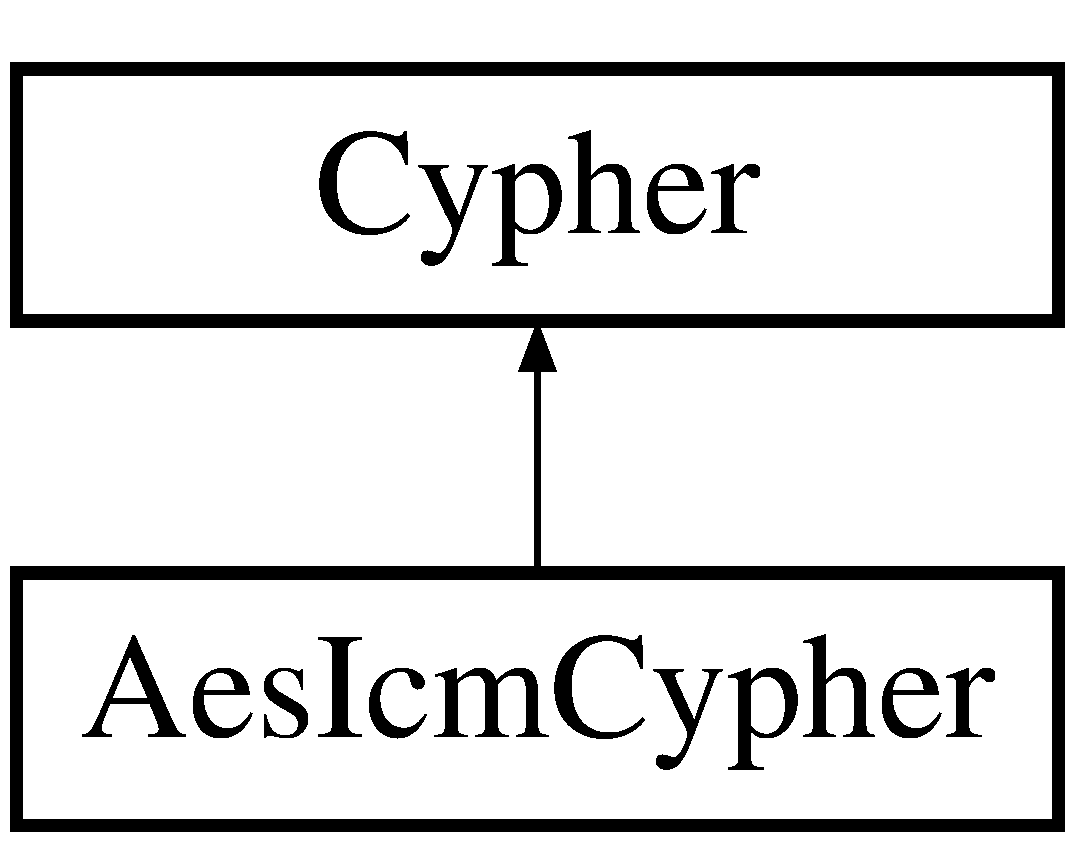
\includegraphics[height=2cm]{classAesIcmCypher}
\end{center}
\end{figure}
\subsection*{Public Member Functions}
\begin{CompactItemize}
\item 
{\bf Aes\-Icm\-Cypher} ()
\item 
{\bf $\sim$Aes\-Icm\-Cypher} ()
\item 
void {\bf set\-Key} ({\bf Buffer} key)
\item 
void {\bf set\-Salt} ({\bf Buffer} salt)
\end{CompactItemize}
\subsection*{Static Public Attributes}
\begin{CompactItemize}
\item 
static const std::string {\bf MIN\_\-GCRYPT\_\-VERSION}
\item 
static const {\bf u\_\-int32\_\-t} {\bf GCRYPT\_\-SEC\_\-MEM}
\end{CompactItemize}
\subsection*{Protected Member Functions}
\begin{CompactItemize}
\item 
{\bf Buffer} {\bf get\-Bit\-Stream} ({\bf u\_\-int32\_\-t} length, {\bf seq\_\-nr\_\-t} seq\_\-nr, {\bf sender\_\-id\_\-t} sender\_\-id)
\end{CompactItemize}
\subsection*{Protected Attributes}
\begin{CompactItemize}
\item 
gcry\_\-cipher\_\-hd\_\-t {\bf cipher\_\-}
\item 
{\bf Buffer} {\bf salt\_\-}
\end{CompactItemize}
\subsection*{Static Private Attributes}
\begin{CompactItemize}
\item 
static bool {\bf gcrypt\_\-initialized\_\-}
\end{CompactItemize}


\subsection{Constructor \& Destructor Documentation}
\index{AesIcmCypher@{Aes\-Icm\-Cypher}!AesIcmCypher@{AesIcmCypher}}
\index{AesIcmCypher@{AesIcmCypher}!AesIcmCypher@{Aes\-Icm\-Cypher}}
\subsubsection{\setlength{\rightskip}{0pt plus 5cm}Aes\-Icm\-Cypher::Aes\-Icm\-Cypher ()}\label{classAesIcmCypher_628abe54d9f3ac715dcaa0ae9ebf44bc}


\index{AesIcmCypher@{Aes\-Icm\-Cypher}!~AesIcmCypher@{$\sim$AesIcmCypher}}
\index{~AesIcmCypher@{$\sim$AesIcmCypher}!AesIcmCypher@{Aes\-Icm\-Cypher}}
\subsubsection{\setlength{\rightskip}{0pt plus 5cm}Aes\-Icm\-Cypher::$\sim$Aes\-Icm\-Cypher ()}\label{classAesIcmCypher_fdf9ab22374ffdad856f172eefacbd17}




\subsection{Member Function Documentation}
\index{AesIcmCypher@{Aes\-Icm\-Cypher}!setKey@{setKey}}
\index{setKey@{setKey}!AesIcmCypher@{Aes\-Icm\-Cypher}}
\subsubsection{\setlength{\rightskip}{0pt plus 5cm}void Aes\-Icm\-Cypher::set\-Key ({\bf Buffer} {\em key})}\label{classAesIcmCypher_605a38676ef12ad0b69628c5d53ef007}




Reimplemented from {\bf Cypher} \doxyref{}{p.}{classCypher_7320b82d14391ab7d25271aa5114e190}.\index{AesIcmCypher@{Aes\-Icm\-Cypher}!setSalt@{setSalt}}
\index{setSalt@{setSalt}!AesIcmCypher@{Aes\-Icm\-Cypher}}
\subsubsection{\setlength{\rightskip}{0pt plus 5cm}void Aes\-Icm\-Cypher::set\-Salt ({\bf Buffer} {\em salt})}\label{classAesIcmCypher_6741487a9d6dfe3ae76bb168ed711259}




Reimplemented from {\bf Cypher} \doxyref{}{p.}{classCypher_2546ef49e5ce8abe8062186d5f6b2ef8}.\index{AesIcmCypher@{Aes\-Icm\-Cypher}!getBitStream@{getBitStream}}
\index{getBitStream@{getBitStream}!AesIcmCypher@{Aes\-Icm\-Cypher}}
\subsubsection{\setlength{\rightskip}{0pt plus 5cm}{\bf Buffer} Aes\-Icm\-Cypher::get\-Bit\-Stream ({\bf u\_\-int32\_\-t} {\em length}, {\bf seq\_\-nr\_\-t} {\em seq\_\-nr}, {\bf sender\_\-id\_\-t} {\em sender\_\-id})\hspace{0.3cm}{\tt  [protected, virtual]}}\label{classAesIcmCypher_ebac1fbb9a4cb56411fcd45ca63f47a1}




Implements {\bf Cypher} \doxyref{}{p.}{classCypher_7ddf1bcd476978daa97148ec406d6483}.

\subsection{Member Data Documentation}
\index{AesIcmCypher@{Aes\-Icm\-Cypher}!MIN_GCRYPT_VERSION@{MIN\_\-GCRYPT\_\-VERSION}}
\index{MIN_GCRYPT_VERSION@{MIN\_\-GCRYPT\_\-VERSION}!AesIcmCypher@{Aes\-Icm\-Cypher}}
\subsubsection{\setlength{\rightskip}{0pt plus 5cm}const std::string {\bf Aes\-Icm\-Cypher::MIN\_\-GCRYPT\_\-VERSION}\hspace{0.3cm}{\tt  [static]}}\label{classAesIcmCypher_605842d12379711d74401d0923b5d76e}


\index{AesIcmCypher@{Aes\-Icm\-Cypher}!GCRYPT_SEC_MEM@{GCRYPT\_\-SEC\_\-MEM}}
\index{GCRYPT_SEC_MEM@{GCRYPT\_\-SEC\_\-MEM}!AesIcmCypher@{Aes\-Icm\-Cypher}}
\subsubsection{\setlength{\rightskip}{0pt plus 5cm}const {\bf u\_\-int32\_\-t} {\bf Aes\-Icm\-Cypher::GCRYPT\_\-SEC\_\-MEM}\hspace{0.3cm}{\tt  [static]}}\label{classAesIcmCypher_4d1dea41b9745bca5a2d84fcefe3558c}


\index{AesIcmCypher@{Aes\-Icm\-Cypher}!cipher_@{cipher\_\-}}
\index{cipher_@{cipher\_\-}!AesIcmCypher@{Aes\-Icm\-Cypher}}
\subsubsection{\setlength{\rightskip}{0pt plus 5cm}gcry\_\-cipher\_\-hd\_\-t {\bf Aes\-Icm\-Cypher::cipher\_\-}\hspace{0.3cm}{\tt  [protected]}}\label{classAesIcmCypher_d74a46baaee2e0755902d134274eac9a}


\index{AesIcmCypher@{Aes\-Icm\-Cypher}!salt_@{salt\_\-}}
\index{salt_@{salt\_\-}!AesIcmCypher@{Aes\-Icm\-Cypher}}
\subsubsection{\setlength{\rightskip}{0pt plus 5cm}{\bf Buffer} {\bf Aes\-Icm\-Cypher::salt\_\-}\hspace{0.3cm}{\tt  [protected]}}\label{classAesIcmCypher_a62620f7280574b142a0eb29880f5083}


\index{AesIcmCypher@{Aes\-Icm\-Cypher}!gcrypt_initialized_@{gcrypt\_\-initialized\_\-}}
\index{gcrypt_initialized_@{gcrypt\_\-initialized\_\-}!AesIcmCypher@{Aes\-Icm\-Cypher}}
\subsubsection{\setlength{\rightskip}{0pt plus 5cm}bool {\bf Aes\-Icm\-Cypher::gcrypt\_\-initialized\_\-}\hspace{0.3cm}{\tt  [static, private]}}\label{classAesIcmCypher_04da5690d9102c6b3fe5bf78a8827ac1}




The documentation for this class was generated from the following files:\begin{CompactItemize}
\item 
{\bf cypher.h}\item 
{\bf cypher.cpp}\end{CompactItemize}

\section{Auth\-Algo Class Reference}
\label{classAuthAlgo}\index{AuthAlgo@{AuthAlgo}}
{\tt \#include $<$auth\-Algo.h$>$}

Inheritance diagram for Auth\-Algo::\begin{figure}[H]
\begin{center}
\leavevmode
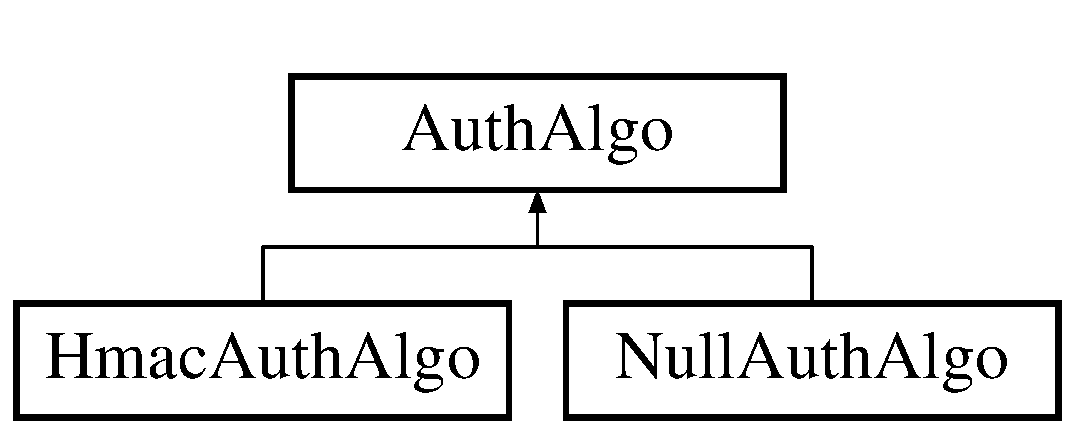
\includegraphics[height=2cm]{classAuthAlgo}
\end{center}
\end{figure}
\subsection*{Public Member Functions}
\begin{CompactItemize}
\item 
{\bf Auth\-Algo} ()
\item 
virtual {\bf $\sim$Auth\-Algo} ()
\item 
virtual {\bf auth\_\-tag\_\-t} {\bf calc} (const {\bf Buffer} \&buf)=0
\end{CompactItemize}


\subsection{Constructor \& Destructor Documentation}
\index{AuthAlgo@{Auth\-Algo}!AuthAlgo@{AuthAlgo}}
\index{AuthAlgo@{AuthAlgo}!AuthAlgo@{Auth\-Algo}}
\subsubsection{\setlength{\rightskip}{0pt plus 5cm}Auth\-Algo::Auth\-Algo ()\hspace{0.3cm}{\tt  [inline]}}\label{classAuthAlgo_22a200c372d9aeb73a4cbdd95ba30a0e}


\index{AuthAlgo@{Auth\-Algo}!~AuthAlgo@{$\sim$AuthAlgo}}
\index{~AuthAlgo@{$\sim$AuthAlgo}!AuthAlgo@{Auth\-Algo}}
\subsubsection{\setlength{\rightskip}{0pt plus 5cm}virtual Auth\-Algo::$\sim$Auth\-Algo ()\hspace{0.3cm}{\tt  [inline, virtual]}}\label{classAuthAlgo_e3428186b4e005e879e26c2b8e04fa4a}




\subsection{Member Function Documentation}
\index{AuthAlgo@{Auth\-Algo}!calc@{calc}}
\index{calc@{calc}!AuthAlgo@{Auth\-Algo}}
\subsubsection{\setlength{\rightskip}{0pt plus 5cm}virtual {\bf auth\_\-tag\_\-t} Auth\-Algo::calc (const {\bf Buffer} \& {\em buf})\hspace{0.3cm}{\tt  [pure virtual]}}\label{classAuthAlgo_f53b44f90c33eb049da260947a75c916}




Implemented in {\bf Null\-Auth\-Algo} \doxyref{}{p.}{classNullAuthAlgo_60eead12d6b32a576ad40d999a6151cf}, and {\bf Hmac\-Auth\-Algo} \doxyref{}{p.}{classHmacAuthAlgo_af50c9aa6b61ff6f4631e3f78f77dc97}.

The documentation for this class was generated from the following file:\begin{CompactItemize}
\item 
{\bf auth\-Algo.h}\end{CompactItemize}

\section{Buffer Class Reference}
\label{classBuffer}\index{Buffer@{Buffer}}
{\tt \#include $<$buffer.h$>$}

Inheritance diagram for Buffer::\begin{figure}[H]
\begin{center}
\leavevmode
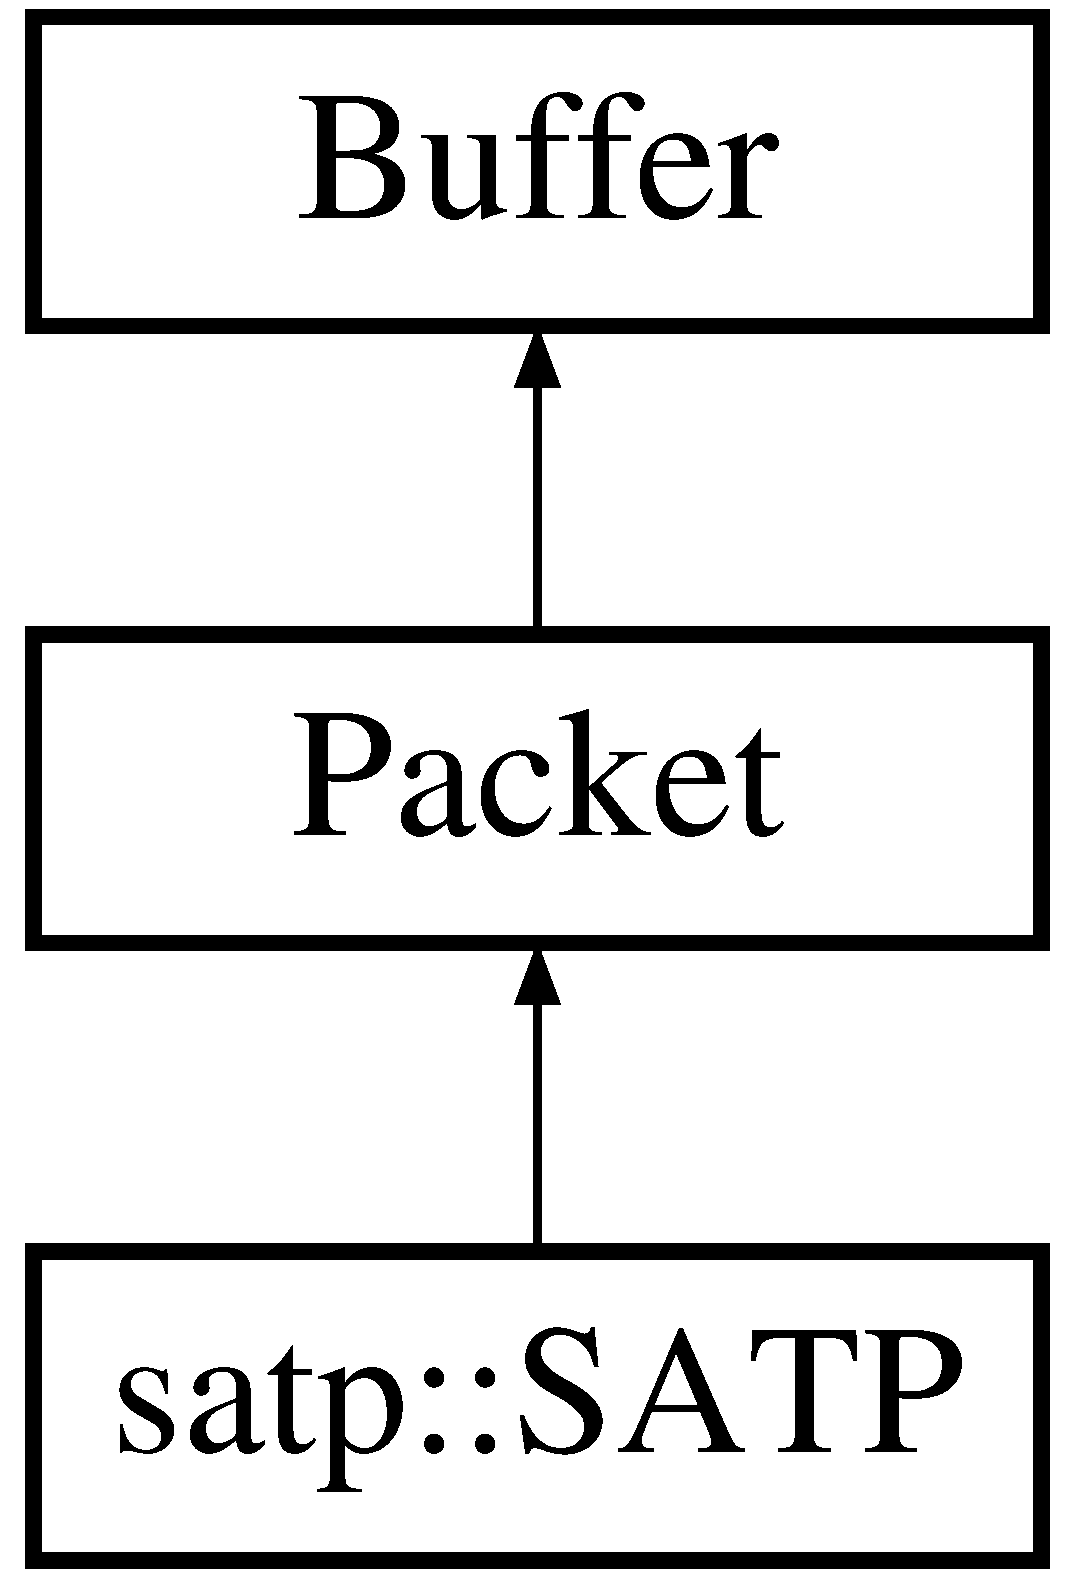
\includegraphics[height=3cm]{classBuffer}
\end{center}
\end{figure}
\subsection*{Public Member Functions}
\begin{CompactItemize}
\item 
{\bf Buffer} ()
\item 
{\bf Buffer} ({\bf u\_\-int32\_\-t} length)
\item 
{\bf Buffer} ({\bf u\_\-int8\_\-t} $\ast$data, {\bf u\_\-int32\_\-t} length)
\item 
virtual {\bf $\sim$Buffer} ()
\item 
{\bf Buffer} (const {\bf Buffer} \&src)
\item 
void {\bf operator=} (const {\bf Buffer} \&src)
\item 
virtual {\bf Buffer} {\bf operator$^\wedge$} (const {\bf Buffer} \&xor\_\-by) const 
\item 
virtual {\bf Buffer} {\bf left\-Byte\-Shift} ({\bf u\_\-int32\_\-t} width) const
\item 
virtual {\bf Buffer} {\bf right\-Byte\-Shift} ({\bf u\_\-int32\_\-t} width) const
\item 
{\bf u\_\-int32\_\-t} {\bf resize\-Front} ({\bf u\_\-int32\_\-t} new\_\-length)
\item 
{\bf u\_\-int32\_\-t} {\bf resize\-Back} ({\bf u\_\-int32\_\-t} new\_\-length)
\item 
{\bf u\_\-int32\_\-t} {\bf get\-Length} () const
\item 
{\bf u\_\-int8\_\-t} $\ast$ {\bf get\-Buf} ()
\item 
{\bf u\_\-int8\_\-t} \& {\bf operator[$\,$]} ({\bf u\_\-int32\_\-t} index)
\item 
{\bf u\_\-int8\_\-t} {\bf operator[$\,$]} ({\bf u\_\-int32\_\-t} index) const
\item 
void {\bf print\-Hex\-Dump} () const
\item 
{\bf operator u\_\-int8\_\-t $\ast$} ()
\end{CompactItemize}
\subsection*{Protected Attributes}
\begin{CompactItemize}
\item 
{\bf u\_\-int8\_\-t} $\ast$ {\bf buf\_\-}
\item 
{\bf u\_\-int32\_\-t} {\bf length\_\-}
\end{CompactItemize}
\subsection*{Friends}
\begin{CompactItemize}
\item 
class {\bf Tun\-Device}
\item 
class {\bf UDPPacket\-Source}
\item 
class {\bf Aes\-Icm\-Cypher}
\item 
class {\bf Key\-Derivation}
\end{CompactItemize}


\subsection{Constructor \& Destructor Documentation}
\index{Buffer@{Buffer}!Buffer@{Buffer}}
\index{Buffer@{Buffer}!Buffer@{Buffer}}
\subsubsection{\setlength{\rightskip}{0pt plus 5cm}Buffer::Buffer ()}\label{classBuffer_e7ef2cd201190fde551dcb902627112b}


\index{Buffer@{Buffer}!Buffer@{Buffer}}
\index{Buffer@{Buffer}!Buffer@{Buffer}}
\subsubsection{\setlength{\rightskip}{0pt plus 5cm}Buffer::Buffer ({\bf u\_\-int32\_\-t} {\em length})}\label{classBuffer_5c58aa9e491f709011408ee7837d57d0}


\index{Buffer@{Buffer}!Buffer@{Buffer}}
\index{Buffer@{Buffer}!Buffer@{Buffer}}
\subsubsection{\setlength{\rightskip}{0pt plus 5cm}Buffer::Buffer ({\bf u\_\-int8\_\-t} $\ast$ {\em data}, {\bf u\_\-int32\_\-t} {\em length})}\label{classBuffer_5bc2edccfb7c1a33354c895ab25c4816}


\index{Buffer@{Buffer}!~Buffer@{$\sim$Buffer}}
\index{~Buffer@{$\sim$Buffer}!Buffer@{Buffer}}
\subsubsection{\setlength{\rightskip}{0pt plus 5cm}Buffer::$\sim$Buffer ()\hspace{0.3cm}{\tt  [virtual]}}\label{classBuffer_59b8743e4a5f731bdd0c4185c9ef263b}


\index{Buffer@{Buffer}!Buffer@{Buffer}}
\index{Buffer@{Buffer}!Buffer@{Buffer}}
\subsubsection{\setlength{\rightskip}{0pt plus 5cm}Buffer::Buffer (const {\bf Buffer} \& {\em src})}\label{classBuffer_042fe5bc1f8d0c25d5707d6955d1654c}




\subsection{Member Function Documentation}
\index{Buffer@{Buffer}!operator=@{operator=}}
\index{operator=@{operator=}!Buffer@{Buffer}}
\subsubsection{\setlength{\rightskip}{0pt plus 5cm}void Buffer::operator= (const {\bf Buffer} \& {\em src})}\label{classBuffer_14cec0d3bf4f3f1a4a9930a8c53eb43a}


\index{Buffer@{Buffer}!operator^@{operator$^\wedge$}}
\index{operator^@{operator$^\wedge$}!Buffer@{Buffer}}
\subsubsection{\setlength{\rightskip}{0pt plus 5cm}{\bf Buffer} Buffer::operator$^\wedge$ (const {\bf Buffer} \& {\em xor\_\-by}) const\hspace{0.3cm}{\tt  [virtual]}}\label{classBuffer_d56159a415541fcff34ef8aed1eb7183}


\index{Buffer@{Buffer}!leftByteShift@{leftByteShift}}
\index{leftByteShift@{leftByteShift}!Buffer@{Buffer}}
\subsubsection{\setlength{\rightskip}{0pt plus 5cm}{\bf Buffer} Buffer::left\-Byte\-Shift ({\bf u\_\-int32\_\-t} {\em width}) const\hspace{0.3cm}{\tt  [virtual]}}\label{classBuffer_13200a4925b1b3c08f99e09ccb6854a1}


\index{Buffer@{Buffer}!rightByteShift@{rightByteShift}}
\index{rightByteShift@{rightByteShift}!Buffer@{Buffer}}
\subsubsection{\setlength{\rightskip}{0pt plus 5cm}{\bf Buffer} Buffer::right\-Byte\-Shift ({\bf u\_\-int32\_\-t} {\em width}) const\hspace{0.3cm}{\tt  [virtual]}}\label{classBuffer_298949899f3f78e4a8b3df7fa5ec532d}


\index{Buffer@{Buffer}!resizeFront@{resizeFront}}
\index{resizeFront@{resizeFront}!Buffer@{Buffer}}
\subsubsection{\setlength{\rightskip}{0pt plus 5cm}{\bf u\_\-int32\_\-t} Buffer::resize\-Front ({\bf u\_\-int32\_\-t} {\em new\_\-length})}\label{classBuffer_fe4b10487b4930e0407bdf61857629d6}


\index{Buffer@{Buffer}!resizeBack@{resizeBack}}
\index{resizeBack@{resizeBack}!Buffer@{Buffer}}
\subsubsection{\setlength{\rightskip}{0pt plus 5cm}{\bf u\_\-int32\_\-t} Buffer::resize\-Back ({\bf u\_\-int32\_\-t} {\em new\_\-length})}\label{classBuffer_5698b2d64238f1f38578dc8e9e2b1bc9}


\index{Buffer@{Buffer}!getLength@{getLength}}
\index{getLength@{getLength}!Buffer@{Buffer}}
\subsubsection{\setlength{\rightskip}{0pt plus 5cm}{\bf u\_\-int32\_\-t} Buffer::get\-Length () const}\label{classBuffer_09ced241e4d0a46c52f0f20398076435}


\index{Buffer@{Buffer}!getBuf@{getBuf}}
\index{getBuf@{getBuf}!Buffer@{Buffer}}
\subsubsection{\setlength{\rightskip}{0pt plus 5cm}{\bf u\_\-int8\_\-t} $\ast$ Buffer::get\-Buf ()}\label{classBuffer_7890e20c6c77eb631c39728ea08b35b8}


\index{Buffer@{Buffer}!operator[]@{operator[]}}
\index{operator[]@{operator[]}!Buffer@{Buffer}}
\subsubsection{\setlength{\rightskip}{0pt plus 5cm}{\bf u\_\-int8\_\-t} \& Buffer::operator[$\,$] ({\bf u\_\-int32\_\-t} {\em index})}\label{classBuffer_763882c627db10206f78b090556b00fa}


\index{Buffer@{Buffer}!operator[]@{operator[]}}
\index{operator[]@{operator[]}!Buffer@{Buffer}}
\subsubsection{\setlength{\rightskip}{0pt plus 5cm}{\bf u\_\-int8\_\-t} Buffer::operator[$\,$] ({\bf u\_\-int32\_\-t} {\em index}) const}\label{classBuffer_e5a9559862374ebd9dfcfc1204890497}


\index{Buffer@{Buffer}!printHexDump@{printHexDump}}
\index{printHexDump@{printHexDump}!Buffer@{Buffer}}
\subsubsection{\setlength{\rightskip}{0pt plus 5cm}void Buffer::print\-Hex\-Dump () const}\label{classBuffer_13d927c471a7516b37bc9ad8fc1741ce}


\index{Buffer@{Buffer}!operator u_int8_t *@{operator u\_\-int8\_\-t $\ast$}}
\index{operator u_int8_t *@{operator u\_\-int8\_\-t $\ast$}!Buffer@{Buffer}}
\subsubsection{\setlength{\rightskip}{0pt plus 5cm}Buffer::operator {\bf u\_\-int8\_\-t} $\ast$ ()}\label{classBuffer_dcf367d5f1b7fced7aa61bb919af7943}




\subsection{Friends And Related Function Documentation}
\index{Buffer@{Buffer}!TunDevice@{TunDevice}}
\index{TunDevice@{TunDevice}!Buffer@{Buffer}}
\subsubsection{\setlength{\rightskip}{0pt plus 5cm}friend class {\bf Tun\-Device}\hspace{0.3cm}{\tt  [friend]}}\label{classBuffer_51b494563d277beb4740f86c519f30fb}


\index{Buffer@{Buffer}!UDPPacketSource@{UDPPacketSource}}
\index{UDPPacketSource@{UDPPacketSource}!Buffer@{Buffer}}
\subsubsection{\setlength{\rightskip}{0pt plus 5cm}friend class {\bf UDPPacket\-Source}\hspace{0.3cm}{\tt  [friend]}}\label{classBuffer_940a382a5e3a8622e6689e13dc453481}


\index{Buffer@{Buffer}!AesIcmCypher@{AesIcmCypher}}
\index{AesIcmCypher@{AesIcmCypher}!Buffer@{Buffer}}
\subsubsection{\setlength{\rightskip}{0pt plus 5cm}friend class {\bf Aes\-Icm\-Cypher}\hspace{0.3cm}{\tt  [friend]}}\label{classBuffer_41d791e5b640813dea34c24c11056581}


\index{Buffer@{Buffer}!KeyDerivation@{KeyDerivation}}
\index{KeyDerivation@{KeyDerivation}!Buffer@{Buffer}}
\subsubsection{\setlength{\rightskip}{0pt plus 5cm}friend class {\bf Key\-Derivation}\hspace{0.3cm}{\tt  [friend]}}\label{classBuffer_1d039eb05e29b8eeadca9b474bb6d49f}




\subsection{Member Data Documentation}
\index{Buffer@{Buffer}!buf_@{buf\_\-}}
\index{buf_@{buf\_\-}!Buffer@{Buffer}}
\subsubsection{\setlength{\rightskip}{0pt plus 5cm}{\bf u\_\-int8\_\-t}$\ast$ {\bf Buffer::buf\_\-}\hspace{0.3cm}{\tt  [protected]}}\label{classBuffer_e60240b77a315e6b3c2bf88592d0be48}


\index{Buffer@{Buffer}!length_@{length\_\-}}
\index{length_@{length\_\-}!Buffer@{Buffer}}
\subsubsection{\setlength{\rightskip}{0pt plus 5cm}{\bf u\_\-int32\_\-t} {\bf Buffer::length\_\-}\hspace{0.3cm}{\tt  [protected]}}\label{classBuffer_d3a779d2403b5183427f12554e2f51c3}




The documentation for this class was generated from the following files:\begin{CompactItemize}
\item 
{\bf buffer.h}\item 
{\bf buffer.cpp}\end{CompactItemize}

\section{Communicating\-Socket Class Reference}
\label{classCommunicatingSocket}\index{CommunicatingSocket@{CommunicatingSocket}}
{\tt \#include $<$Practical\-Socket.h$>$}

Inheritance diagram for Communicating\-Socket::\begin{figure}[H]
\begin{center}
\leavevmode
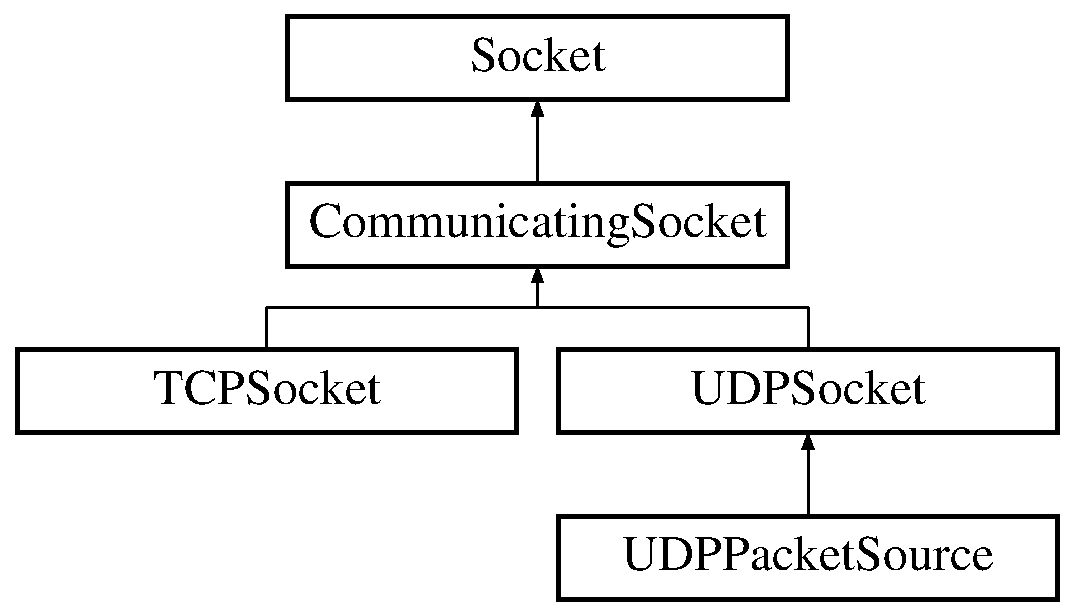
\includegraphics[height=4cm]{classCommunicatingSocket}
\end{center}
\end{figure}
\subsection*{Public Member Functions}
\begin{CompactItemize}
\item 
void {\bf connect} (const string \&foreign\-Address, unsigned short foreign\-Port)  throw (Socket\-Exception)
\item 
void {\bf send} (const void $\ast$buffer, int buffer\-Len)  throw (Socket\-Exception)
\item 
int {\bf recv} (void $\ast$buffer, int buffer\-Len)  throw (Socket\-Exception)
\item 
string {\bf get\-Foreign\-Address} ()  throw (Socket\-Exception)
\item 
unsigned short {\bf get\-Foreign\-Port} ()  throw (Socket\-Exception)
\end{CompactItemize}
\subsection*{Protected Member Functions}
\begin{CompactItemize}
\item 
{\bf Communicating\-Socket} (int type, int protocol)  throw (Socket\-Exception)
\item 
{\bf Communicating\-Socket} (int new\-Conn\-SD)
\end{CompactItemize}


\subsection{Detailed Description}
\doxyref{Socket}{p.}{classSocket} which is able to connect, send, and receive 



\subsection{Constructor \& Destructor Documentation}
\index{CommunicatingSocket@{Communicating\-Socket}!CommunicatingSocket@{CommunicatingSocket}}
\index{CommunicatingSocket@{CommunicatingSocket}!CommunicatingSocket@{Communicating\-Socket}}
\subsubsection{\setlength{\rightskip}{0pt plus 5cm}Communicating\-Socket::Communicating\-Socket (int {\em type}, int {\em protocol})  throw ({\bf Socket\-Exception})\hspace{0.3cm}{\tt  [protected]}}\label{classCommunicatingSocket_0017517b8d6e761fde0c40475af3b2ab}


\index{CommunicatingSocket@{Communicating\-Socket}!CommunicatingSocket@{CommunicatingSocket}}
\index{CommunicatingSocket@{CommunicatingSocket}!CommunicatingSocket@{Communicating\-Socket}}
\subsubsection{\setlength{\rightskip}{0pt plus 5cm}Communicating\-Socket::Communicating\-Socket (int {\em new\-Conn\-SD})\hspace{0.3cm}{\tt  [protected]}}\label{classCommunicatingSocket_27d758db782b3be7d28741e92cb613d1}




\subsection{Member Function Documentation}
\index{CommunicatingSocket@{Communicating\-Socket}!connect@{connect}}
\index{connect@{connect}!CommunicatingSocket@{Communicating\-Socket}}
\subsubsection{\setlength{\rightskip}{0pt plus 5cm}void Communicating\-Socket::connect (const string \& {\em foreign\-Address}, unsigned short {\em foreign\-Port})  throw ({\bf Socket\-Exception})}\label{classCommunicatingSocket_9192374d9baab8e189860aa8d913683c}


Establish a socket connection with the given foreign address and port \begin{Desc}
\item[Parameters:]
\begin{description}
\item[{\em foreign\-Address}]foreign address (IP address or name) \item[{\em foreign\-Port}]foreign port \end{description}
\end{Desc}
\begin{Desc}
\item[Exceptions:]
\begin{description}
\item[{\em \doxyref{Socket\-Exception}{p.}{classSocketException}}]thrown if unable to establish connection \end{description}
\end{Desc}
\index{CommunicatingSocket@{Communicating\-Socket}!send@{send}}
\index{send@{send}!CommunicatingSocket@{Communicating\-Socket}}
\subsubsection{\setlength{\rightskip}{0pt plus 5cm}void Communicating\-Socket::send (const void $\ast$ {\em buffer}, int {\em buffer\-Len})  throw ({\bf Socket\-Exception})}\label{classCommunicatingSocket_ca4e86085c064641e86ae24ea29bbb94}


Write the given buffer to this socket. Call \doxyref{connect()}{p.}{classCommunicatingSocket_9192374d9baab8e189860aa8d913683c} before calling \doxyref{send()}{p.}{classCommunicatingSocket_ca4e86085c064641e86ae24ea29bbb94} \begin{Desc}
\item[Parameters:]
\begin{description}
\item[{\em buffer}]buffer to be written \item[{\em buffer\-Len}]number of bytes from buffer to be written \end{description}
\end{Desc}
\begin{Desc}
\item[Exceptions:]
\begin{description}
\item[{\em \doxyref{Socket\-Exception}{p.}{classSocketException}}]thrown if unable to send data \end{description}
\end{Desc}
\index{CommunicatingSocket@{Communicating\-Socket}!recv@{recv}}
\index{recv@{recv}!CommunicatingSocket@{Communicating\-Socket}}
\subsubsection{\setlength{\rightskip}{0pt plus 5cm}int Communicating\-Socket::recv (void $\ast$ {\em buffer}, int {\em buffer\-Len})  throw ({\bf Socket\-Exception})}\label{classCommunicatingSocket_7cf1fd470c0060171b68df9f68c7bd01}


Read into the given buffer up to buffer\-Len bytes data from this socket. Call \doxyref{connect()}{p.}{classCommunicatingSocket_9192374d9baab8e189860aa8d913683c} before calling \doxyref{recv()}{p.}{classCommunicatingSocket_7cf1fd470c0060171b68df9f68c7bd01} \begin{Desc}
\item[Parameters:]
\begin{description}
\item[{\em buffer}]buffer to receive the data \item[{\em buffer\-Len}]maximum number of bytes to read into buffer \end{description}
\end{Desc}
\begin{Desc}
\item[Returns:]number of bytes read, 0 for EOF, and -1 for error \end{Desc}
\begin{Desc}
\item[Exceptions:]
\begin{description}
\item[{\em \doxyref{Socket\-Exception}{p.}{classSocketException}}]thrown if unable to receive data \end{description}
\end{Desc}
\index{CommunicatingSocket@{Communicating\-Socket}!getForeignAddress@{getForeignAddress}}
\index{getForeignAddress@{getForeignAddress}!CommunicatingSocket@{Communicating\-Socket}}
\subsubsection{\setlength{\rightskip}{0pt plus 5cm}string Communicating\-Socket::get\-Foreign\-Address ()  throw ({\bf Socket\-Exception})}\label{classCommunicatingSocket_13f9eca30ef56836cf23c163c848c09e}


Get the foreign address. Call \doxyref{connect()}{p.}{classCommunicatingSocket_9192374d9baab8e189860aa8d913683c} before calling \doxyref{recv()}{p.}{classCommunicatingSocket_7cf1fd470c0060171b68df9f68c7bd01} \begin{Desc}
\item[Returns:]foreign address \end{Desc}
\begin{Desc}
\item[Exceptions:]
\begin{description}
\item[{\em \doxyref{Socket\-Exception}{p.}{classSocketException}}]thrown if unable to fetch foreign address \end{description}
\end{Desc}
\index{CommunicatingSocket@{Communicating\-Socket}!getForeignPort@{getForeignPort}}
\index{getForeignPort@{getForeignPort}!CommunicatingSocket@{Communicating\-Socket}}
\subsubsection{\setlength{\rightskip}{0pt plus 5cm}unsigned short Communicating\-Socket::get\-Foreign\-Port ()  throw ({\bf Socket\-Exception})}\label{classCommunicatingSocket_184fbb4775184b87ebd886a5587eb1a3}


Get the foreign port. Call \doxyref{connect()}{p.}{classCommunicatingSocket_9192374d9baab8e189860aa8d913683c} before calling \doxyref{recv()}{p.}{classCommunicatingSocket_7cf1fd470c0060171b68df9f68c7bd01} \begin{Desc}
\item[Returns:]foreign port \end{Desc}
\begin{Desc}
\item[Exceptions:]
\begin{description}
\item[{\em \doxyref{Socket\-Exception}{p.}{classSocketException}}]thrown if unable to fetch foreign port \end{description}
\end{Desc}


The documentation for this class was generated from the following files:\begin{CompactItemize}
\item 
{\bf Practical\-Socket.h}\item 
{\bf Practical\-Socket.cpp}\end{CompactItemize}

\section{Condition Class Reference}
\label{classCondition}\index{Condition@{Condition}}
{\tt \#include $<$thread\-Utils.hpp$>$}

\subsection*{Public Member Functions}
\begin{CompactItemize}
\item 
{\bf Condition} ()
\item 
{\bf $\sim$Condition} ()
\item 
void {\bf wait} ()
\item 
void {\bf signal} ()
\item 
void {\bf broadcast} ()
\end{CompactItemize}
\subsection*{Private Attributes}
\begin{CompactItemize}
\item 
pthread\_\-cond\_\-t {\bf cond}
\item 
{\bf Mutex} {\bf mutex}
\end{CompactItemize}


\subsection{Constructor \& Destructor Documentation}
\index{Condition@{Condition}!Condition@{Condition}}
\index{Condition@{Condition}!Condition@{Condition}}
\subsubsection{\setlength{\rightskip}{0pt plus 5cm}Condition::Condition ()\hspace{0.3cm}{\tt  [inline]}}\label{classCondition_f11513db4fcbde93961fa0b65e7ab764}


\index{Condition@{Condition}!~Condition@{$\sim$Condition}}
\index{~Condition@{$\sim$Condition}!Condition@{Condition}}
\subsubsection{\setlength{\rightskip}{0pt plus 5cm}Condition::$\sim$Condition ()\hspace{0.3cm}{\tt  [inline]}}\label{classCondition_b42f6d2dfb2d0de4bed4ed5032d4a8fc}




\subsection{Member Function Documentation}
\index{Condition@{Condition}!wait@{wait}}
\index{wait@{wait}!Condition@{Condition}}
\subsubsection{\setlength{\rightskip}{0pt plus 5cm}void Condition::wait ()\hspace{0.3cm}{\tt  [inline]}}\label{classCondition_0bb9ca22c3c755d0ed8c7483a857567a}


\index{Condition@{Condition}!signal@{signal}}
\index{signal@{signal}!Condition@{Condition}}
\subsubsection{\setlength{\rightskip}{0pt plus 5cm}void Condition::signal ()\hspace{0.3cm}{\tt  [inline]}}\label{classCondition_974c8fd419e6014028dc4147cc49ce56}


\index{Condition@{Condition}!broadcast@{broadcast}}
\index{broadcast@{broadcast}!Condition@{Condition}}
\subsubsection{\setlength{\rightskip}{0pt plus 5cm}void Condition::broadcast ()\hspace{0.3cm}{\tt  [inline]}}\label{classCondition_15d88ea71e837f967d13d805d675cc5b}




\subsection{Member Data Documentation}
\index{Condition@{Condition}!cond@{cond}}
\index{cond@{cond}!Condition@{Condition}}
\subsubsection{\setlength{\rightskip}{0pt plus 5cm}pthread\_\-cond\_\-t {\bf Condition::cond}\hspace{0.3cm}{\tt  [private]}}\label{classCondition_4c8982005641d63b696f671b28e3706d}


\index{Condition@{Condition}!mutex@{mutex}}
\index{mutex@{mutex}!Condition@{Condition}}
\subsubsection{\setlength{\rightskip}{0pt plus 5cm}{\bf Mutex} {\bf Condition::mutex}\hspace{0.3cm}{\tt  [private]}}\label{classCondition_01622814c6a21250677c2b9cbfc86bfb}




The documentation for this class was generated from the following file:\begin{CompactItemize}
\item 
{\bf thread\-Utils.hpp}\end{CompactItemize}

\include{classConnectionList}
\include{classConnectionParam}
\section{Cypher Class Reference}
\label{classCypher}\index{Cypher@{Cypher}}
{\tt \#include $<$cypher.h$>$}

Inheritance diagram for Cypher::\begin{figure}[H]
\begin{center}
\leavevmode
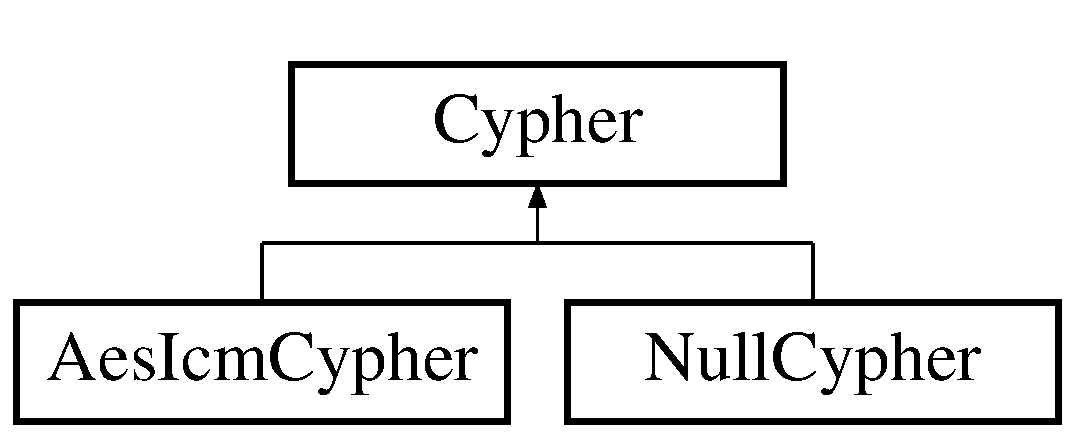
\includegraphics[height=2cm]{classCypher}
\end{center}
\end{figure}
\subsection*{Public Member Functions}
\begin{CompactItemize}
\item 
{\bf Cypher} ()
\item 
virtual {\bf $\sim$Cypher} ()
\item 
void {\bf set\-Key} ({\bf Buffer} key)
\item 
void {\bf set\-Salt} ({\bf Buffer} salt)
\item 
void {\bf cypher} ({\bf Buffer} \&buf, {\bf seq\_\-nr\_\-t} seq\_\-nr, {\bf sender\_\-id\_\-t} sender\_\-id)
\end{CompactItemize}
\subsection*{Protected Member Functions}
\begin{CompactItemize}
\item 
void {\bf exor} ({\bf Buffer} \&buf, const {\bf Buffer} \&bit\_\-stream)
\item 
virtual {\bf Buffer} {\bf get\-Bit\-Stream} ({\bf u\_\-int32\_\-t} length, {\bf seq\_\-nr\_\-t} seq\_\-nr, {\bf sender\_\-id\_\-t} sender\_\-id)=0
\end{CompactItemize}


\subsection{Constructor \& Destructor Documentation}
\index{Cypher@{Cypher}!Cypher@{Cypher}}
\index{Cypher@{Cypher}!Cypher@{Cypher}}
\subsubsection{\setlength{\rightskip}{0pt plus 5cm}Cypher::Cypher ()\hspace{0.3cm}{\tt  [inline]}}\label{classCypher_5228228b0b2d83251ecce4516e87ddb1}


\index{Cypher@{Cypher}!~Cypher@{$\sim$Cypher}}
\index{~Cypher@{$\sim$Cypher}!Cypher@{Cypher}}
\subsubsection{\setlength{\rightskip}{0pt plus 5cm}virtual Cypher::$\sim$Cypher ()\hspace{0.3cm}{\tt  [inline, virtual]}}\label{classCypher_70c94525f7bacb956cdd940fba7fb4c8}




\subsection{Member Function Documentation}
\index{Cypher@{Cypher}!setKey@{setKey}}
\index{setKey@{setKey}!Cypher@{Cypher}}
\subsubsection{\setlength{\rightskip}{0pt plus 5cm}void Cypher::set\-Key ({\bf Buffer} {\em key})\hspace{0.3cm}{\tt  [inline]}}\label{classCypher_7320b82d14391ab7d25271aa5114e190}




Reimplemented in {\bf Aes\-Icm\-Cypher} \doxyref{}{p.}{classAesIcmCypher_605a38676ef12ad0b69628c5d53ef007}.\index{Cypher@{Cypher}!setSalt@{setSalt}}
\index{setSalt@{setSalt}!Cypher@{Cypher}}
\subsubsection{\setlength{\rightskip}{0pt plus 5cm}void Cypher::set\-Salt ({\bf Buffer} {\em salt})\hspace{0.3cm}{\tt  [inline]}}\label{classCypher_2546ef49e5ce8abe8062186d5f6b2ef8}




Reimplemented in {\bf Aes\-Icm\-Cypher} \doxyref{}{p.}{classAesIcmCypher_6741487a9d6dfe3ae76bb168ed711259}.\index{Cypher@{Cypher}!cypher@{cypher}}
\index{cypher@{cypher}!Cypher@{Cypher}}
\subsubsection{\setlength{\rightskip}{0pt plus 5cm}void Cypher::cypher ({\bf Buffer} \& {\em buf}, {\bf seq\_\-nr\_\-t} {\em seq\_\-nr}, {\bf sender\_\-id\_\-t} {\em sender\_\-id})}\label{classCypher_1d51ce2235d38bded45f5e897be4435c}


\index{Cypher@{Cypher}!exor@{exor}}
\index{exor@{exor}!Cypher@{Cypher}}
\subsubsection{\setlength{\rightskip}{0pt plus 5cm}void Cypher::exor ({\bf Buffer} \& {\em buf}, const {\bf Buffer} \& {\em bit\_\-stream})\hspace{0.3cm}{\tt  [protected]}}\label{classCypher_bf33a7a59ed1cdf711030236de6635b0}


\index{Cypher@{Cypher}!getBitStream@{getBitStream}}
\index{getBitStream@{getBitStream}!Cypher@{Cypher}}
\subsubsection{\setlength{\rightskip}{0pt plus 5cm}virtual {\bf Buffer} Cypher::get\-Bit\-Stream ({\bf u\_\-int32\_\-t} {\em length}, {\bf seq\_\-nr\_\-t} {\em seq\_\-nr}, {\bf sender\_\-id\_\-t} {\em sender\_\-id})\hspace{0.3cm}{\tt  [protected, pure virtual]}}\label{classCypher_7ddf1bcd476978daa97148ec406d6483}




Implemented in {\bf Null\-Cypher} \doxyref{}{p.}{classNullCypher_ca537adca8ea9af8b6f248df12ebcf36}, and {\bf Aes\-Icm\-Cypher} \doxyref{}{p.}{classAesIcmCypher_ebac1fbb9a4cb56411fcd45ca63f47a1}.

The documentation for this class was generated from the following files:\begin{CompactItemize}
\item 
{\bf cypher.h}\item 
{\bf cypher.cpp}\end{CompactItemize}

\section{Hmac\-Auth\-Algo Class Reference}
\label{classHmacAuthAlgo}\index{HmacAuthAlgo@{HmacAuthAlgo}}
{\tt \#include $<$auth\-Algo.h$>$}

Inheritance diagram for Hmac\-Auth\-Algo::\begin{figure}[H]
\begin{center}
\leavevmode
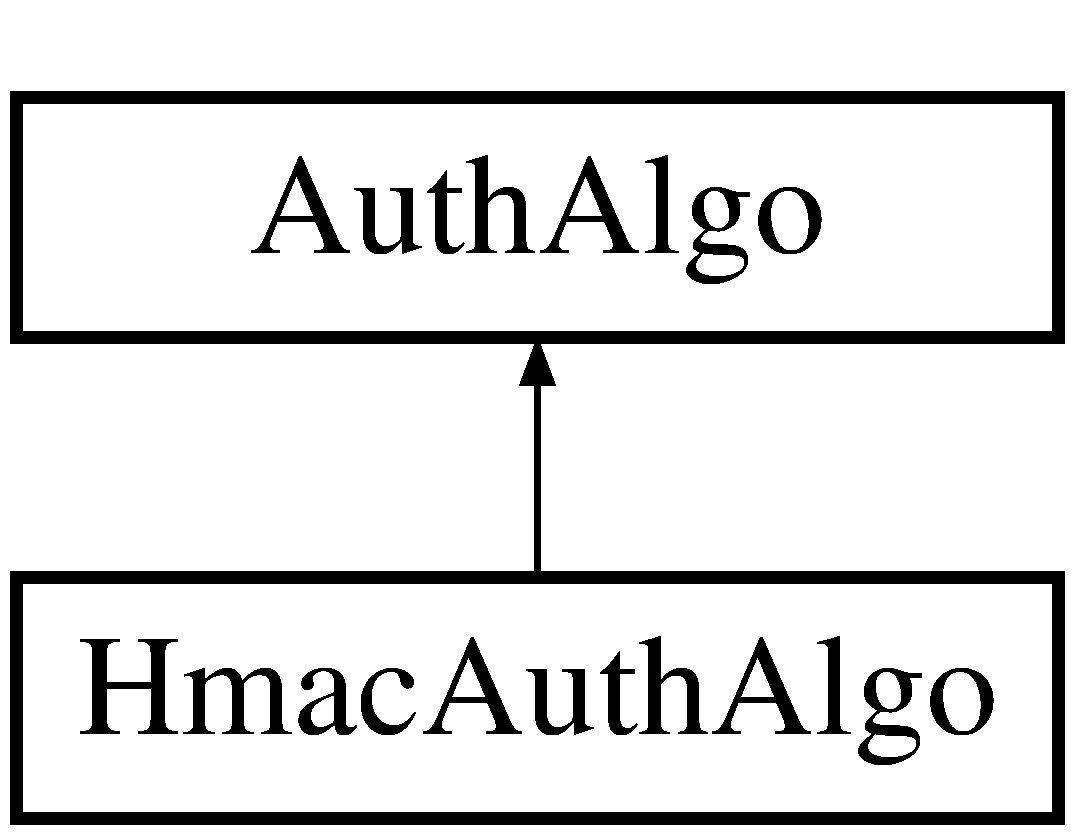
\includegraphics[height=2cm]{classHmacAuthAlgo}
\end{center}
\end{figure}
\subsection*{Public Member Functions}
\begin{CompactItemize}
\item 
{\bf auth\_\-tag\_\-t} {\bf calc} (const {\bf Buffer} \&buf)
\end{CompactItemize}


\subsection{Member Function Documentation}
\index{HmacAuthAlgo@{Hmac\-Auth\-Algo}!calc@{calc}}
\index{calc@{calc}!HmacAuthAlgo@{Hmac\-Auth\-Algo}}
\subsubsection{\setlength{\rightskip}{0pt plus 5cm}{\bf auth\_\-tag\_\-t} Hmac\-Auth\-Algo::calc (const {\bf Buffer} \& {\em buf})\hspace{0.3cm}{\tt  [virtual]}}\label{classHmacAuthAlgo_af50c9aa6b61ff6f4631e3f78f77dc97}




Implements {\bf Auth\-Algo} \doxyref{}{p.}{classAuthAlgo_f53b44f90c33eb049da260947a75c916}.

The documentation for this class was generated from the following files:\begin{CompactItemize}
\item 
{\bf auth\-Algo.h}\item 
{\bf auth\-Algo.cpp}\end{CompactItemize}

\section{Key\-Derivation Class Reference}
\label{classKeyDerivation}\index{KeyDerivation@{KeyDerivation}}
{\tt \#include $<$key\-Derivation.h$>$}

\subsection*{Public Member Functions}
\begin{CompactItemize}
\item 
{\bf Key\-Derivation} ()
\item 
virtual {\bf $\sim$Key\-Derivation} ()
\item 
void {\bf init} ({\bf Buffer} key, {\bf Buffer} salt)
\item 
void {\bf set\-Log\-KDRate} (const {\bf u\_\-int8\_\-t} ld\_\-rate)
\item 
void {\bf generate} ({\bf satp\_\-prf\_\-label} label, {\bf seq\_\-nr\_\-t} seq\_\-nr, {\bf Buffer} \&key, {\bf u\_\-int32\_\-t} length)
\item 
void {\bf clear} ()
\end{CompactItemize}
\subsection*{Protected Attributes}
\begin{CompactItemize}
\item 
{\bf int8\_\-t} {\bf ld\_\-kdr\_\-}
\item 
{\bf Buffer} {\bf salt\_\-}
\item 
gcry\_\-cipher\_\-hd\_\-t {\bf cipher\_\-}
\end{CompactItemize}
\subsection*{Static Protected Attributes}
\begin{CompactItemize}
\item 
static const char $\ast$ {\bf MIN\_\-GCRYPT\_\-VERSION}
\end{CompactItemize}


\subsection{Constructor \& Destructor Documentation}
\index{KeyDerivation@{Key\-Derivation}!KeyDerivation@{KeyDerivation}}
\index{KeyDerivation@{KeyDerivation}!KeyDerivation@{Key\-Derivation}}
\subsubsection{\setlength{\rightskip}{0pt plus 5cm}Key\-Derivation::Key\-Derivation ()\hspace{0.3cm}{\tt  [inline]}}\label{classKeyDerivation_07c3735d1b2e1285b6c427a2706ebc67}


\index{KeyDerivation@{Key\-Derivation}!~KeyDerivation@{$\sim$KeyDerivation}}
\index{~KeyDerivation@{$\sim$KeyDerivation}!KeyDerivation@{Key\-Derivation}}
\subsubsection{\setlength{\rightskip}{0pt plus 5cm}virtual Key\-Derivation::$\sim$Key\-Derivation ()\hspace{0.3cm}{\tt  [inline, virtual]}}\label{classKeyDerivation_ccce2c32370be2388ca0a977fef1f6cc}




\subsection{Member Function Documentation}
\index{KeyDerivation@{Key\-Derivation}!init@{init}}
\index{init@{init}!KeyDerivation@{Key\-Derivation}}
\subsubsection{\setlength{\rightskip}{0pt plus 5cm}void Key\-Derivation::init ({\bf Buffer} {\em key}, {\bf Buffer} {\em salt})}\label{classKeyDerivation_5f03e97de1a041f6012d1fcfabf13773}


\index{KeyDerivation@{Key\-Derivation}!setLogKDRate@{setLogKDRate}}
\index{setLogKDRate@{setLogKDRate}!KeyDerivation@{Key\-Derivation}}
\subsubsection{\setlength{\rightskip}{0pt plus 5cm}void Key\-Derivation::set\-Log\-KDRate (const {\bf u\_\-int8\_\-t} {\em ld\_\-rate})}\label{classKeyDerivation_b055afc0de04a6e32631e42f09b32e63}


\index{KeyDerivation@{Key\-Derivation}!generate@{generate}}
\index{generate@{generate}!KeyDerivation@{Key\-Derivation}}
\subsubsection{\setlength{\rightskip}{0pt plus 5cm}void Key\-Derivation::generate ({\bf satp\_\-prf\_\-label} {\em label}, {\bf seq\_\-nr\_\-t} {\em seq\_\-nr}, {\bf Buffer} \& {\em key}, {\bf u\_\-int32\_\-t} {\em length})}\label{classKeyDerivation_6d319febcad73d199fe8773ae614f70a}


\index{KeyDerivation@{Key\-Derivation}!clear@{clear}}
\index{clear@{clear}!KeyDerivation@{Key\-Derivation}}
\subsubsection{\setlength{\rightskip}{0pt plus 5cm}void Key\-Derivation::clear ()}\label{classKeyDerivation_8d8c405ee7c3753b4807b36a8cbe537a}




\subsection{Member Data Documentation}
\index{KeyDerivation@{Key\-Derivation}!ld_kdr_@{ld\_\-kdr\_\-}}
\index{ld_kdr_@{ld\_\-kdr\_\-}!KeyDerivation@{Key\-Derivation}}
\subsubsection{\setlength{\rightskip}{0pt plus 5cm}{\bf int8\_\-t} {\bf Key\-Derivation::ld\_\-kdr\_\-}\hspace{0.3cm}{\tt  [protected]}}\label{classKeyDerivation_426dcd34d3b60191a3db55dd970eeb17}


\index{KeyDerivation@{Key\-Derivation}!salt_@{salt\_\-}}
\index{salt_@{salt\_\-}!KeyDerivation@{Key\-Derivation}}
\subsubsection{\setlength{\rightskip}{0pt plus 5cm}{\bf Buffer} {\bf Key\-Derivation::salt\_\-}\hspace{0.3cm}{\tt  [protected]}}\label{classKeyDerivation_52e057f1085920a61ea44c5c9936865c}


\index{KeyDerivation@{Key\-Derivation}!MIN_GCRYPT_VERSION@{MIN\_\-GCRYPT\_\-VERSION}}
\index{MIN_GCRYPT_VERSION@{MIN\_\-GCRYPT\_\-VERSION}!KeyDerivation@{Key\-Derivation}}
\subsubsection{\setlength{\rightskip}{0pt plus 5cm}const char $\ast$ {\bf Key\-Derivation::MIN\_\-GCRYPT\_\-VERSION}\hspace{0.3cm}{\tt  [static, protected]}}\label{classKeyDerivation_2091534e962a9d0f7b3b034150d33333}


\index{KeyDerivation@{Key\-Derivation}!cipher_@{cipher\_\-}}
\index{cipher_@{cipher\_\-}!KeyDerivation@{Key\-Derivation}}
\subsubsection{\setlength{\rightskip}{0pt plus 5cm}gcry\_\-cipher\_\-hd\_\-t {\bf Key\-Derivation::cipher\_\-}\hspace{0.3cm}{\tt  [protected]}}\label{classKeyDerivation_6b7dd9a922de96a8f76cf6c453adab28}




The documentation for this class was generated from the following files:\begin{CompactItemize}
\item 
{\bf key\-Derivation.h}\item 
{\bf key\-Derivation.cpp}\end{CompactItemize}

\section{Lock Class Reference}
\label{classLock}\index{Lock@{Lock}}
{\tt \#include $<$thread\-Utils.hpp$>$}

\subsection*{Public Member Functions}
\begin{CompactItemize}
\item 
{\bf Lock} ({\bf Mutex} \&m)
\item 
{\bf $\sim$Lock} ()
\end{CompactItemize}
\subsection*{Private Member Functions}
\begin{CompactItemize}
\item 
{\bf Lock} (const {\bf Lock} \&src)
\item 
void {\bf operator=} (const {\bf Lock} \&src)
\end{CompactItemize}
\subsection*{Private Attributes}
\begin{CompactItemize}
\item 
{\bf Mutex} \& {\bf mutex}
\end{CompactItemize}


\subsection{Constructor \& Destructor Documentation}
\index{Lock@{Lock}!Lock@{Lock}}
\index{Lock@{Lock}!Lock@{Lock}}
\subsubsection{\setlength{\rightskip}{0pt plus 5cm}Lock::Lock ({\bf Mutex} \& {\em m})\hspace{0.3cm}{\tt  [inline]}}\label{classLock_2c786576eddddb484a6a02a7dea52904}


\index{Lock@{Lock}!~Lock@{$\sim$Lock}}
\index{~Lock@{$\sim$Lock}!Lock@{Lock}}
\subsubsection{\setlength{\rightskip}{0pt plus 5cm}Lock::$\sim$Lock ()\hspace{0.3cm}{\tt  [inline]}}\label{classLock_7ab6d9485c8665bb3643710432882971}


\index{Lock@{Lock}!Lock@{Lock}}
\index{Lock@{Lock}!Lock@{Lock}}
\subsubsection{\setlength{\rightskip}{0pt plus 5cm}Lock::Lock (const {\bf Lock} \& {\em src})\hspace{0.3cm}{\tt  [private]}}\label{classLock_5aba40fb170cf8fbfbe241ecac4b66b2}




\subsection{Member Function Documentation}
\index{Lock@{Lock}!operator=@{operator=}}
\index{operator=@{operator=}!Lock@{Lock}}
\subsubsection{\setlength{\rightskip}{0pt plus 5cm}void Lock::operator= (const {\bf Lock} \& {\em src})\hspace{0.3cm}{\tt  [private]}}\label{classLock_6beb534a89b213d70e4b3bb9b3cde217}




\subsection{Member Data Documentation}
\index{Lock@{Lock}!mutex@{mutex}}
\index{mutex@{mutex}!Lock@{Lock}}
\subsubsection{\setlength{\rightskip}{0pt plus 5cm}{\bf Mutex}\& {\bf Lock::mutex}\hspace{0.3cm}{\tt  [private]}}\label{classLock_41f8817641e260bddb93a7a710736037}




The documentation for this class was generated from the following file:\begin{CompactItemize}
\item 
{\bf thread\-Utils.hpp}\end{CompactItemize}

\section{Log Class Reference}
\label{classLog}\index{Log@{Log}}
{\tt \#include $<$log.h$>$}

\subsection*{Public Member Functions}
\begin{CompactItemize}
\item 
{\bf Log} \& {\bf set\-Log\-Name} (std::string new\-Log\-Name)
\item 
std::string {\bf get\-Log\-Name} () const
\item 
{\bf Log} \& {\bf set\-Facility} (int new\-Facility)
\item 
int {\bf get\-Facility} () const
\item 
{\bf Log\-String\-Builder} {\bf msg} (int prio={\bf PRIO\_\-INFO})
\end{CompactItemize}
\subsection*{Static Public Member Functions}
\begin{CompactItemize}
\item 
static {\bf Log} \& {\bf instance} ()
\end{CompactItemize}
\subsection*{Static Public Attributes}
\begin{CompactItemize}
\item 
static const int {\bf FAC\_\-USER} = LOG\_\-USER
\item 
static const int {\bf FAC\_\-MAIL} = LOG\_\-MAIL
\item 
static const int {\bf FAC\_\-DAEMON} = LOG\_\-DAEMON
\item 
static const int {\bf FAC\_\-AUTH} = LOG\_\-AUTH
\item 
static const int {\bf FAC\_\-SYSLOG} = LOG\_\-SYSLOG
\item 
static const int {\bf FAC\_\-LPR} = LOG\_\-LPR
\item 
static const int {\bf FAC\_\-NEWS} = LOG\_\-NEWS
\item 
static const int {\bf FAC\_\-UUCP} = LOG\_\-UUCP
\item 
static const int {\bf FAC\_\-CRON} = LOG\_\-CRON
\item 
static const int {\bf FAC\_\-AUTHPRIV} = LOG\_\-AUTHPRIV
\item 
static const int {\bf FAC\_\-FTP} = LOG\_\-FTP
\item 
static const int {\bf FAC\_\-LOCAL0} = LOG\_\-LOCAL0
\item 
static const int {\bf FAC\_\-LOCAL1} = LOG\_\-LOCAL1
\item 
static const int {\bf FAC\_\-LOCAL2} = LOG\_\-LOCAL2
\item 
static const int {\bf FAC\_\-LOCAL3} = LOG\_\-LOCAL3
\item 
static const int {\bf FAC\_\-LOCAL4} = LOG\_\-LOCAL4
\item 
static const int {\bf FAC\_\-LOCAL5} = LOG\_\-LOCAL5
\item 
static const int {\bf FAC\_\-LOCAL6} = LOG\_\-LOCAL6
\item 
static const int {\bf FAC\_\-LOCAL7} = LOG\_\-LOCAL7
\item 
static const int {\bf PRIO\_\-EMERG} = LOG\_\-EMERG
\item 
static const int {\bf PRIO\_\-ALERT} = LOG\_\-ALERT
\item 
static const int {\bf PRIO\_\-CRIT} = LOG\_\-CRIT
\item 
static const int {\bf PRIO\_\-ERR} = LOG\_\-ERR
\item 
static const int {\bf PRIO\_\-WARNING} = LOG\_\-WARNING
\item 
static const int {\bf PRIO\_\-NOTICE} = LOG\_\-NOTICE
\item 
static const int {\bf PRIO\_\-INFO} = LOG\_\-INFO
\item 
static const int {\bf PRIO\_\-DEBUG} = LOG\_\-DEBUG
\end{CompactItemize}
\subsection*{Private Member Functions}
\begin{CompactItemize}
\item 
{\bf Log} ()
\item 
{\bf $\sim$Log} ()
\item 
{\bf Log} (const {\bf Log} \&l)
\item 
void {\bf operator=} (const {\bf Log} \&l)
\item 
void {\bf open} ()
\end{CompactItemize}
\subsection*{Private Attributes}
\begin{CompactItemize}
\item 
{\bf Mutex} {\bf mutex}
\item 
std::string {\bf log\-Name}
\item 
int {\bf facility}
\end{CompactItemize}
\subsection*{Static Private Attributes}
\begin{CompactItemize}
\item 
static {\bf Log} $\ast$ {\bf inst}
\item 
static {\bf Mutex} {\bf inst\-Mutex}
\end{CompactItemize}
\subsection*{Friends}
\begin{CompactItemize}
\item 
class {\bf instance\-Cleaner}
\item 
class {\bf Log\-String\-Builder}
\end{CompactItemize}
\subsection*{Classes}
\begin{CompactItemize}
\item 
class {\bf instance\-Cleaner}
\end{CompactItemize}


\subsection{Constructor \& Destructor Documentation}
\index{Log@{Log}!Log@{Log}}
\index{Log@{Log}!Log@{Log}}
\subsubsection{\setlength{\rightskip}{0pt plus 5cm}Log::Log ()\hspace{0.3cm}{\tt  [private]}}\label{classLog_f6071a60aa52b6c1b511f99b4bc1b8fe}


\index{Log@{Log}!~Log@{$\sim$Log}}
\index{~Log@{$\sim$Log}!Log@{Log}}
\subsubsection{\setlength{\rightskip}{0pt plus 5cm}Log::$\sim$Log ()\hspace{0.3cm}{\tt  [private]}}\label{classLog_0fbfda88fbee5027c89f6eb121059360}


\index{Log@{Log}!Log@{Log}}
\index{Log@{Log}!Log@{Log}}
\subsubsection{\setlength{\rightskip}{0pt plus 5cm}Log::Log (const {\bf Log} \& {\em l})\hspace{0.3cm}{\tt  [private]}}\label{classLog_756aec21ec377fbc703f787e7f5fb832}




\subsection{Member Function Documentation}
\index{Log@{Log}!instance@{instance}}
\index{instance@{instance}!Log@{Log}}
\subsubsection{\setlength{\rightskip}{0pt plus 5cm}{\bf Log} \& Log::instance ()\hspace{0.3cm}{\tt  [static]}}\label{classLog_aa59866ce9e78db15ce7aaeb00fc1063}


\index{Log@{Log}!setLogName@{setLogName}}
\index{setLogName@{setLogName}!Log@{Log}}
\subsubsection{\setlength{\rightskip}{0pt plus 5cm}{\bf Log} \& Log::set\-Log\-Name (std::string {\em new\-Log\-Name})}\label{classLog_f8cf0541a8284aabd5fe924a9cd2eab8}


\index{Log@{Log}!getLogName@{getLogName}}
\index{getLogName@{getLogName}!Log@{Log}}
\subsubsection{\setlength{\rightskip}{0pt plus 5cm}std::string Log::get\-Log\-Name () const\hspace{0.3cm}{\tt  [inline]}}\label{classLog_9090c0fbbc5a3223dbd361a827788c17}


\index{Log@{Log}!setFacility@{setFacility}}
\index{setFacility@{setFacility}!Log@{Log}}
\subsubsection{\setlength{\rightskip}{0pt plus 5cm}{\bf Log} \& Log::set\-Facility (int {\em new\-Facility})}\label{classLog_828e15ec0e9108b9fc43d74da77a902c}


\index{Log@{Log}!getFacility@{getFacility}}
\index{getFacility@{getFacility}!Log@{Log}}
\subsubsection{\setlength{\rightskip}{0pt plus 5cm}int Log::get\-Facility () const\hspace{0.3cm}{\tt  [inline]}}\label{classLog_238b6e5d47bb83307737f0c809fad669}


\index{Log@{Log}!msg@{msg}}
\index{msg@{msg}!Log@{Log}}
\subsubsection{\setlength{\rightskip}{0pt plus 5cm}{\bf Log\-String\-Builder} Log::msg (int {\em prio} = {\tt {\bf PRIO\_\-INFO}})\hspace{0.3cm}{\tt  [inline]}}\label{classLog_7077dc047eb915d2fae46e36f5040f85}


\index{Log@{Log}!operator=@{operator=}}
\index{operator=@{operator=}!Log@{Log}}
\subsubsection{\setlength{\rightskip}{0pt plus 5cm}void Log::operator= (const {\bf Log} \& {\em l})\hspace{0.3cm}{\tt  [private]}}\label{classLog_076b147c2bc9b2167074e9bc51a24af7}


\index{Log@{Log}!open@{open}}
\index{open@{open}!Log@{Log}}
\subsubsection{\setlength{\rightskip}{0pt plus 5cm}void Log::open ()\hspace{0.3cm}{\tt  [private]}}\label{classLog_f91976ebadd955414799131cb442d24c}




\subsection{Friends And Related Function Documentation}
\index{Log@{Log}!instanceCleaner@{instanceCleaner}}
\index{instanceCleaner@{instanceCleaner}!Log@{Log}}
\subsubsection{\setlength{\rightskip}{0pt plus 5cm}friend class {\bf instance\-Cleaner}\hspace{0.3cm}{\tt  [friend]}}\label{classLog_321cfbf9f58ebf3c9366bd6e0b5c18ce}


\index{Log@{Log}!LogStringBuilder@{LogStringBuilder}}
\index{LogStringBuilder@{LogStringBuilder}!Log@{Log}}
\subsubsection{\setlength{\rightskip}{0pt plus 5cm}friend class {\bf Log\-String\-Builder}\hspace{0.3cm}{\tt  [friend]}}\label{classLog_16ded253dbe65c503d1d853dcf5460d6}




\subsection{Member Data Documentation}
\index{Log@{Log}!FAC_USER@{FAC\_\-USER}}
\index{FAC_USER@{FAC\_\-USER}!Log@{Log}}
\subsubsection{\setlength{\rightskip}{0pt plus 5cm}const int {\bf Log::FAC\_\-USER} = LOG\_\-USER\hspace{0.3cm}{\tt  [static]}}\label{classLog_9418bab5d66822411ce1f85823d8425b}


\index{Log@{Log}!FAC_MAIL@{FAC\_\-MAIL}}
\index{FAC_MAIL@{FAC\_\-MAIL}!Log@{Log}}
\subsubsection{\setlength{\rightskip}{0pt plus 5cm}const int {\bf Log::FAC\_\-MAIL} = LOG\_\-MAIL\hspace{0.3cm}{\tt  [static]}}\label{classLog_5cf4b465d8ecff58bd62ac064663917b}


\index{Log@{Log}!FAC_DAEMON@{FAC\_\-DAEMON}}
\index{FAC_DAEMON@{FAC\_\-DAEMON}!Log@{Log}}
\subsubsection{\setlength{\rightskip}{0pt plus 5cm}const int {\bf Log::FAC\_\-DAEMON} = LOG\_\-DAEMON\hspace{0.3cm}{\tt  [static]}}\label{classLog_6395030c0b8fa7f36b6fe0f6b837055d}


\index{Log@{Log}!FAC_AUTH@{FAC\_\-AUTH}}
\index{FAC_AUTH@{FAC\_\-AUTH}!Log@{Log}}
\subsubsection{\setlength{\rightskip}{0pt plus 5cm}const int {\bf Log::FAC\_\-AUTH} = LOG\_\-AUTH\hspace{0.3cm}{\tt  [static]}}\label{classLog_6f6fde7b6433d827c05cfefe16f9b333}


\index{Log@{Log}!FAC_SYSLOG@{FAC\_\-SYSLOG}}
\index{FAC_SYSLOG@{FAC\_\-SYSLOG}!Log@{Log}}
\subsubsection{\setlength{\rightskip}{0pt plus 5cm}const int {\bf Log::FAC\_\-SYSLOG} = LOG\_\-SYSLOG\hspace{0.3cm}{\tt  [static]}}\label{classLog_be74100156fee45add0417bc9f460f30}


\index{Log@{Log}!FAC_LPR@{FAC\_\-LPR}}
\index{FAC_LPR@{FAC\_\-LPR}!Log@{Log}}
\subsubsection{\setlength{\rightskip}{0pt plus 5cm}const int {\bf Log::FAC\_\-LPR} = LOG\_\-LPR\hspace{0.3cm}{\tt  [static]}}\label{classLog_28a1239643de68f79ad6c2337acfd2ea}


\index{Log@{Log}!FAC_NEWS@{FAC\_\-NEWS}}
\index{FAC_NEWS@{FAC\_\-NEWS}!Log@{Log}}
\subsubsection{\setlength{\rightskip}{0pt plus 5cm}const int {\bf Log::FAC\_\-NEWS} = LOG\_\-NEWS\hspace{0.3cm}{\tt  [static]}}\label{classLog_b9f56520aeae70b9d98396f67ad1310b}


\index{Log@{Log}!FAC_UUCP@{FAC\_\-UUCP}}
\index{FAC_UUCP@{FAC\_\-UUCP}!Log@{Log}}
\subsubsection{\setlength{\rightskip}{0pt plus 5cm}const int {\bf Log::FAC\_\-UUCP} = LOG\_\-UUCP\hspace{0.3cm}{\tt  [static]}}\label{classLog_d5b2e5f3987835ec077013c6a263ed5f}


\index{Log@{Log}!FAC_CRON@{FAC\_\-CRON}}
\index{FAC_CRON@{FAC\_\-CRON}!Log@{Log}}
\subsubsection{\setlength{\rightskip}{0pt plus 5cm}const int {\bf Log::FAC\_\-CRON} = LOG\_\-CRON\hspace{0.3cm}{\tt  [static]}}\label{classLog_6a455dfca6d859f77ed79b6d92ad659a}


\index{Log@{Log}!FAC_AUTHPRIV@{FAC\_\-AUTHPRIV}}
\index{FAC_AUTHPRIV@{FAC\_\-AUTHPRIV}!Log@{Log}}
\subsubsection{\setlength{\rightskip}{0pt plus 5cm}const int {\bf Log::FAC\_\-AUTHPRIV} = LOG\_\-AUTHPRIV\hspace{0.3cm}{\tt  [static]}}\label{classLog_5245bb60b9c33e31027ea1f9a77d8053}


\index{Log@{Log}!FAC_FTP@{FAC\_\-FTP}}
\index{FAC_FTP@{FAC\_\-FTP}!Log@{Log}}
\subsubsection{\setlength{\rightskip}{0pt plus 5cm}const int {\bf Log::FAC\_\-FTP} = LOG\_\-FTP\hspace{0.3cm}{\tt  [static]}}\label{classLog_9b822438fee8c8a0f4bb56c0e4415c95}


\index{Log@{Log}!FAC_LOCAL0@{FAC\_\-LOCAL0}}
\index{FAC_LOCAL0@{FAC\_\-LOCAL0}!Log@{Log}}
\subsubsection{\setlength{\rightskip}{0pt plus 5cm}const int {\bf Log::FAC\_\-LOCAL0} = LOG\_\-LOCAL0\hspace{0.3cm}{\tt  [static]}}\label{classLog_e6271aefc4c8749e602da64f284f0d08}


\index{Log@{Log}!FAC_LOCAL1@{FAC\_\-LOCAL1}}
\index{FAC_LOCAL1@{FAC\_\-LOCAL1}!Log@{Log}}
\subsubsection{\setlength{\rightskip}{0pt plus 5cm}const int {\bf Log::FAC\_\-LOCAL1} = LOG\_\-LOCAL1\hspace{0.3cm}{\tt  [static]}}\label{classLog_b553df5af8dd47f2e9d29569b26b7713}


\index{Log@{Log}!FAC_LOCAL2@{FAC\_\-LOCAL2}}
\index{FAC_LOCAL2@{FAC\_\-LOCAL2}!Log@{Log}}
\subsubsection{\setlength{\rightskip}{0pt plus 5cm}const int {\bf Log::FAC\_\-LOCAL2} = LOG\_\-LOCAL2\hspace{0.3cm}{\tt  [static]}}\label{classLog_1e79b43d3ed6f44281f1d6f4d6e2a829}


\index{Log@{Log}!FAC_LOCAL3@{FAC\_\-LOCAL3}}
\index{FAC_LOCAL3@{FAC\_\-LOCAL3}!Log@{Log}}
\subsubsection{\setlength{\rightskip}{0pt plus 5cm}const int {\bf Log::FAC\_\-LOCAL3} = LOG\_\-LOCAL3\hspace{0.3cm}{\tt  [static]}}\label{classLog_467961bf9b0b73dd863a29e29642ed62}


\index{Log@{Log}!FAC_LOCAL4@{FAC\_\-LOCAL4}}
\index{FAC_LOCAL4@{FAC\_\-LOCAL4}!Log@{Log}}
\subsubsection{\setlength{\rightskip}{0pt plus 5cm}const int {\bf Log::FAC\_\-LOCAL4} = LOG\_\-LOCAL4\hspace{0.3cm}{\tt  [static]}}\label{classLog_2dfec8266dc4bfd9f4a37a6a6a193724}


\index{Log@{Log}!FAC_LOCAL5@{FAC\_\-LOCAL5}}
\index{FAC_LOCAL5@{FAC\_\-LOCAL5}!Log@{Log}}
\subsubsection{\setlength{\rightskip}{0pt plus 5cm}const int {\bf Log::FAC\_\-LOCAL5} = LOG\_\-LOCAL5\hspace{0.3cm}{\tt  [static]}}\label{classLog_8c8f287b845408f62e9971869764193d}


\index{Log@{Log}!FAC_LOCAL6@{FAC\_\-LOCAL6}}
\index{FAC_LOCAL6@{FAC\_\-LOCAL6}!Log@{Log}}
\subsubsection{\setlength{\rightskip}{0pt plus 5cm}const int {\bf Log::FAC\_\-LOCAL6} = LOG\_\-LOCAL6\hspace{0.3cm}{\tt  [static]}}\label{classLog_c7c45c9e1daa96ecb60ff12064a3dc6e}


\index{Log@{Log}!FAC_LOCAL7@{FAC\_\-LOCAL7}}
\index{FAC_LOCAL7@{FAC\_\-LOCAL7}!Log@{Log}}
\subsubsection{\setlength{\rightskip}{0pt plus 5cm}const int {\bf Log::FAC\_\-LOCAL7} = LOG\_\-LOCAL7\hspace{0.3cm}{\tt  [static]}}\label{classLog_886a44fb4cec033f0f7c028f530fe97c}


\index{Log@{Log}!PRIO_EMERG@{PRIO\_\-EMERG}}
\index{PRIO_EMERG@{PRIO\_\-EMERG}!Log@{Log}}
\subsubsection{\setlength{\rightskip}{0pt plus 5cm}const int {\bf Log::PRIO\_\-EMERG} = LOG\_\-EMERG\hspace{0.3cm}{\tt  [static]}}\label{classLog_3b068a7b9c9a7bd3a42d519daea16564}


\index{Log@{Log}!PRIO_ALERT@{PRIO\_\-ALERT}}
\index{PRIO_ALERT@{PRIO\_\-ALERT}!Log@{Log}}
\subsubsection{\setlength{\rightskip}{0pt plus 5cm}const int {\bf Log::PRIO\_\-ALERT} = LOG\_\-ALERT\hspace{0.3cm}{\tt  [static]}}\label{classLog_77741b4b68493a7b082f856c9a70cae6}


\index{Log@{Log}!PRIO_CRIT@{PRIO\_\-CRIT}}
\index{PRIO_CRIT@{PRIO\_\-CRIT}!Log@{Log}}
\subsubsection{\setlength{\rightskip}{0pt plus 5cm}const int {\bf Log::PRIO\_\-CRIT} = LOG\_\-CRIT\hspace{0.3cm}{\tt  [static]}}\label{classLog_275d2db1310f0b9663ac1e048cadd389}


\index{Log@{Log}!PRIO_ERR@{PRIO\_\-ERR}}
\index{PRIO_ERR@{PRIO\_\-ERR}!Log@{Log}}
\subsubsection{\setlength{\rightskip}{0pt plus 5cm}const int {\bf Log::PRIO\_\-ERR} = LOG\_\-ERR\hspace{0.3cm}{\tt  [static]}}\label{classLog_d3769cb6592629a056ffeaa4ce1f3d46}


\index{Log@{Log}!PRIO_WARNING@{PRIO\_\-WARNING}}
\index{PRIO_WARNING@{PRIO\_\-WARNING}!Log@{Log}}
\subsubsection{\setlength{\rightskip}{0pt plus 5cm}const int {\bf Log::PRIO\_\-WARNING} = LOG\_\-WARNING\hspace{0.3cm}{\tt  [static]}}\label{classLog_ef36517c65a41f4cf69d4795ec84b4a2}


\index{Log@{Log}!PRIO_NOTICE@{PRIO\_\-NOTICE}}
\index{PRIO_NOTICE@{PRIO\_\-NOTICE}!Log@{Log}}
\subsubsection{\setlength{\rightskip}{0pt plus 5cm}const int {\bf Log::PRIO\_\-NOTICE} = LOG\_\-NOTICE\hspace{0.3cm}{\tt  [static]}}\label{classLog_783504697beb7cc8905d0296704d62f2}


\index{Log@{Log}!PRIO_INFO@{PRIO\_\-INFO}}
\index{PRIO_INFO@{PRIO\_\-INFO}!Log@{Log}}
\subsubsection{\setlength{\rightskip}{0pt plus 5cm}const int {\bf Log::PRIO\_\-INFO} = LOG\_\-INFO\hspace{0.3cm}{\tt  [static]}}\label{classLog_3c50bb6ae5eff66436d72a53c50b0f6b}


\index{Log@{Log}!PRIO_DEBUG@{PRIO\_\-DEBUG}}
\index{PRIO_DEBUG@{PRIO\_\-DEBUG}!Log@{Log}}
\subsubsection{\setlength{\rightskip}{0pt plus 5cm}const int {\bf Log::PRIO\_\-DEBUG} = LOG\_\-DEBUG\hspace{0.3cm}{\tt  [static]}}\label{classLog_f9aad3521e9eda1c156009188cc0674b}


\index{Log@{Log}!inst@{inst}}
\index{inst@{inst}!Log@{Log}}
\subsubsection{\setlength{\rightskip}{0pt plus 5cm}{\bf Log} $\ast$ {\bf Log::inst}\hspace{0.3cm}{\tt  [static, private]}}\label{classLog_aebf3ec6bf45b97cc842d9d53a5a6c0a}


\index{Log@{Log}!instMutex@{instMutex}}
\index{instMutex@{instMutex}!Log@{Log}}
\subsubsection{\setlength{\rightskip}{0pt plus 5cm}{\bf Mutex} {\bf Log::inst\-Mutex}\hspace{0.3cm}{\tt  [static, private]}}\label{classLog_c561e8206daad55b4aa4ac8808f35314}


\index{Log@{Log}!mutex@{mutex}}
\index{mutex@{mutex}!Log@{Log}}
\subsubsection{\setlength{\rightskip}{0pt plus 5cm}{\bf Mutex} {\bf Log::mutex}\hspace{0.3cm}{\tt  [private]}}\label{classLog_d69b96c96c1b6aa0c3d67e07ca131e85}


\index{Log@{Log}!logName@{logName}}
\index{logName@{logName}!Log@{Log}}
\subsubsection{\setlength{\rightskip}{0pt plus 5cm}std::string {\bf Log::log\-Name}\hspace{0.3cm}{\tt  [private]}}\label{classLog_8abf9fa58d7af501f25415eb37fd71a0}


\index{Log@{Log}!facility@{facility}}
\index{facility@{facility}!Log@{Log}}
\subsubsection{\setlength{\rightskip}{0pt plus 5cm}int {\bf Log::facility}\hspace{0.3cm}{\tt  [private]}}\label{classLog_844dc5894a51dce933ae2109868652a0}




The documentation for this class was generated from the following files:\begin{CompactItemize}
\item 
{\bf log.h}\item 
{\bf log.cpp}\end{CompactItemize}

\section{Log::instance\-Cleaner Class Reference}
\label{classLog_1_1instanceCleaner}\index{Log::instanceCleaner@{Log::instanceCleaner}}
\subsection*{Public Member Functions}
\begin{CompactItemize}
\item 
{\bf $\sim$instance\-Cleaner} ()
\end{CompactItemize}


\subsection{Constructor \& Destructor Documentation}
\index{Log::instanceCleaner@{Log::instance\-Cleaner}!~instanceCleaner@{$\sim$instanceCleaner}}
\index{~instanceCleaner@{$\sim$instanceCleaner}!Log::instanceCleaner@{Log::instance\-Cleaner}}
\subsubsection{\setlength{\rightskip}{0pt plus 5cm}Log::instance\-Cleaner::$\sim$instance\-Cleaner ()\hspace{0.3cm}{\tt  [inline]}}\label{classLog_1_1instanceCleaner_5e2dd96e4f58345bd2067cd40fbec865}




The documentation for this class was generated from the following file:\begin{CompactItemize}
\item 
{\bf log.h}\end{CompactItemize}

\section{Log\-String\-Builder Class Reference}
\label{classLogStringBuilder}\index{LogStringBuilder@{LogStringBuilder}}
{\tt \#include $<$log.h$>$}

\subsection*{Public Member Functions}
\begin{CompactItemize}
\item 
{\bf Log\-String\-Builder} ({\bf Log\-String\-Builder} const \&src)
\item 
{\bf Log\-String\-Builder} ({\bf Log} \&l, int p)
\item 
{\bf $\sim$Log\-String\-Builder} ()
\item 
template$<$class T$>$ std::ostream \& {\bf operator$<$$<$} (T const \&value)
\end{CompactItemize}
\subsection*{Private Attributes}
\begin{CompactItemize}
\item 
{\bf Log} \& {\bf log}
\item 
int {\bf prio}
\item 
std::stringstream {\bf stream}
\end{CompactItemize}


\subsection{Constructor \& Destructor Documentation}
\index{LogStringBuilder@{Log\-String\-Builder}!LogStringBuilder@{LogStringBuilder}}
\index{LogStringBuilder@{LogStringBuilder}!LogStringBuilder@{Log\-String\-Builder}}
\subsubsection{\setlength{\rightskip}{0pt plus 5cm}Log\-String\-Builder::Log\-String\-Builder ({\bf Log\-String\-Builder} const \& {\em src})}\label{classLogStringBuilder_5df8c8d7ab7615c8552de3d4d21d3417}


\index{LogStringBuilder@{Log\-String\-Builder}!LogStringBuilder@{LogStringBuilder}}
\index{LogStringBuilder@{LogStringBuilder}!LogStringBuilder@{Log\-String\-Builder}}
\subsubsection{\setlength{\rightskip}{0pt plus 5cm}Log\-String\-Builder::Log\-String\-Builder ({\bf Log} \& {\em l}, int {\em p})}\label{classLogStringBuilder_a9393394f93ca644c8a851fb8fe04e24}


\index{LogStringBuilder@{Log\-String\-Builder}!~LogStringBuilder@{$\sim$LogStringBuilder}}
\index{~LogStringBuilder@{$\sim$LogStringBuilder}!LogStringBuilder@{Log\-String\-Builder}}
\subsubsection{\setlength{\rightskip}{0pt plus 5cm}Log\-String\-Builder::$\sim$Log\-String\-Builder ()}\label{classLogStringBuilder_c63707864e0005008cc4a67d8dec9933}




\subsection{Member Function Documentation}
\index{LogStringBuilder@{Log\-String\-Builder}!operator<<@{operator$<$$<$}}
\index{operator<<@{operator$<$$<$}!LogStringBuilder@{Log\-String\-Builder}}
\subsubsection{\setlength{\rightskip}{0pt plus 5cm}template$<$class T$>$ std::ostream\& Log\-String\-Builder::operator$<$$<$ (T const \& {\em value})\hspace{0.3cm}{\tt  [inline]}}\label{classLogStringBuilder_9b4f26f5e64aacc172c0818073117e42}




\subsection{Member Data Documentation}
\index{LogStringBuilder@{Log\-String\-Builder}!log@{log}}
\index{log@{log}!LogStringBuilder@{Log\-String\-Builder}}
\subsubsection{\setlength{\rightskip}{0pt plus 5cm}{\bf Log}\& {\bf Log\-String\-Builder::log}\hspace{0.3cm}{\tt  [private]}}\label{classLogStringBuilder_499c5b058df61e2215368592d21aacf1}


\index{LogStringBuilder@{Log\-String\-Builder}!prio@{prio}}
\index{prio@{prio}!LogStringBuilder@{Log\-String\-Builder}}
\subsubsection{\setlength{\rightskip}{0pt plus 5cm}int {\bf Log\-String\-Builder::prio}\hspace{0.3cm}{\tt  [private]}}\label{classLogStringBuilder_89d48a7590de117fec0b40c0babbaee5}


\index{LogStringBuilder@{Log\-String\-Builder}!stream@{stream}}
\index{stream@{stream}!LogStringBuilder@{Log\-String\-Builder}}
\subsubsection{\setlength{\rightskip}{0pt plus 5cm}std::stringstream {\bf Log\-String\-Builder::stream}\hspace{0.3cm}{\tt  [private]}}\label{classLogStringBuilder_405447561d3d7337cc093dad6c6d81b5}




The documentation for this class was generated from the following files:\begin{CompactItemize}
\item 
{\bf log.h}\item 
{\bf log.cpp}\end{CompactItemize}

\section{Mutex Class Reference}
\label{classMutex}\index{Mutex@{Mutex}}
{\tt \#include $<$thread\-Utils.hpp$>$}

\subsection*{Public Member Functions}
\begin{CompactItemize}
\item 
{\bf Mutex} ()
\item 
{\bf $\sim$Mutex} ()
\end{CompactItemize}
\subsection*{Private Member Functions}
\begin{CompactItemize}
\item 
{\bf Mutex} (const {\bf Mutex} \&src)
\item 
void {\bf operator=} (const {\bf Mutex} \&src)
\item 
void {\bf lock} ()
\item 
void {\bf unlock} ()
\end{CompactItemize}
\subsection*{Private Attributes}
\begin{CompactItemize}
\item 
pthread\_\-mutex\_\-t {\bf mutex}
\end{CompactItemize}
\subsection*{Friends}
\begin{CompactItemize}
\item 
class {\bf Lock}
\item 
class {\bf Condition}
\end{CompactItemize}


\subsection{Constructor \& Destructor Documentation}
\index{Mutex@{Mutex}!Mutex@{Mutex}}
\index{Mutex@{Mutex}!Mutex@{Mutex}}
\subsubsection{\setlength{\rightskip}{0pt plus 5cm}Mutex::Mutex ()\hspace{0.3cm}{\tt  [inline]}}\label{classMutex_593423d868daf926c7b0d63a833ae29a}


\index{Mutex@{Mutex}!~Mutex@{$\sim$Mutex}}
\index{~Mutex@{$\sim$Mutex}!Mutex@{Mutex}}
\subsubsection{\setlength{\rightskip}{0pt plus 5cm}Mutex::$\sim$Mutex ()\hspace{0.3cm}{\tt  [inline]}}\label{classMutex_c9e9182407f5f74892318607888e9be4}


\index{Mutex@{Mutex}!Mutex@{Mutex}}
\index{Mutex@{Mutex}!Mutex@{Mutex}}
\subsubsection{\setlength{\rightskip}{0pt plus 5cm}Mutex::Mutex (const {\bf Mutex} \& {\em src})\hspace{0.3cm}{\tt  [private]}}\label{classMutex_7f1ad3a125c7a02b2ca338240bd1d978}




\subsection{Member Function Documentation}
\index{Mutex@{Mutex}!operator=@{operator=}}
\index{operator=@{operator=}!Mutex@{Mutex}}
\subsubsection{\setlength{\rightskip}{0pt plus 5cm}void Mutex::operator= (const {\bf Mutex} \& {\em src})\hspace{0.3cm}{\tt  [private]}}\label{classMutex_030a11400d00ef97813c6b232a5e3f43}


\index{Mutex@{Mutex}!lock@{lock}}
\index{lock@{lock}!Mutex@{Mutex}}
\subsubsection{\setlength{\rightskip}{0pt plus 5cm}void Mutex::lock ()\hspace{0.3cm}{\tt  [inline, private]}}\label{classMutex_d91be808bf0a60a16f10b897ec246d3a}


\index{Mutex@{Mutex}!unlock@{unlock}}
\index{unlock@{unlock}!Mutex@{Mutex}}
\subsubsection{\setlength{\rightskip}{0pt plus 5cm}void Mutex::unlock ()\hspace{0.3cm}{\tt  [inline, private]}}\label{classMutex_546a5b797ba29959357586aa2b3740a8}




\subsection{Friends And Related Function Documentation}
\index{Mutex@{Mutex}!Lock@{Lock}}
\index{Lock@{Lock}!Mutex@{Mutex}}
\subsubsection{\setlength{\rightskip}{0pt plus 5cm}friend class {\bf Lock}\hspace{0.3cm}{\tt  [friend]}}\label{classMutex_5bf7608e05250fb524a1229bcf83ece3}


\index{Mutex@{Mutex}!Condition@{Condition}}
\index{Condition@{Condition}!Mutex@{Mutex}}
\subsubsection{\setlength{\rightskip}{0pt plus 5cm}friend class {\bf Condition}\hspace{0.3cm}{\tt  [friend]}}\label{classMutex_0705c7682858f6dcf7fe85cba92f0a5c}




\subsection{Member Data Documentation}
\index{Mutex@{Mutex}!mutex@{mutex}}
\index{mutex@{mutex}!Mutex@{Mutex}}
\subsubsection{\setlength{\rightskip}{0pt plus 5cm}pthread\_\-mutex\_\-t {\bf Mutex::mutex}\hspace{0.3cm}{\tt  [private]}}\label{classMutex_8feb0b01916c1feedd1f0c0dcd74081b}




The documentation for this class was generated from the following file:\begin{CompactItemize}
\item 
{\bf thread\-Utils.hpp}\end{CompactItemize}

\include{classNetworkAddress}
\section{Null\-Auth\-Algo Class Reference}
\label{classNullAuthAlgo}\index{NullAuthAlgo@{NullAuthAlgo}}
{\tt \#include $<$auth\-Algo.h$>$}

Inheritance diagram for Null\-Auth\-Algo::\begin{figure}[H]
\begin{center}
\leavevmode
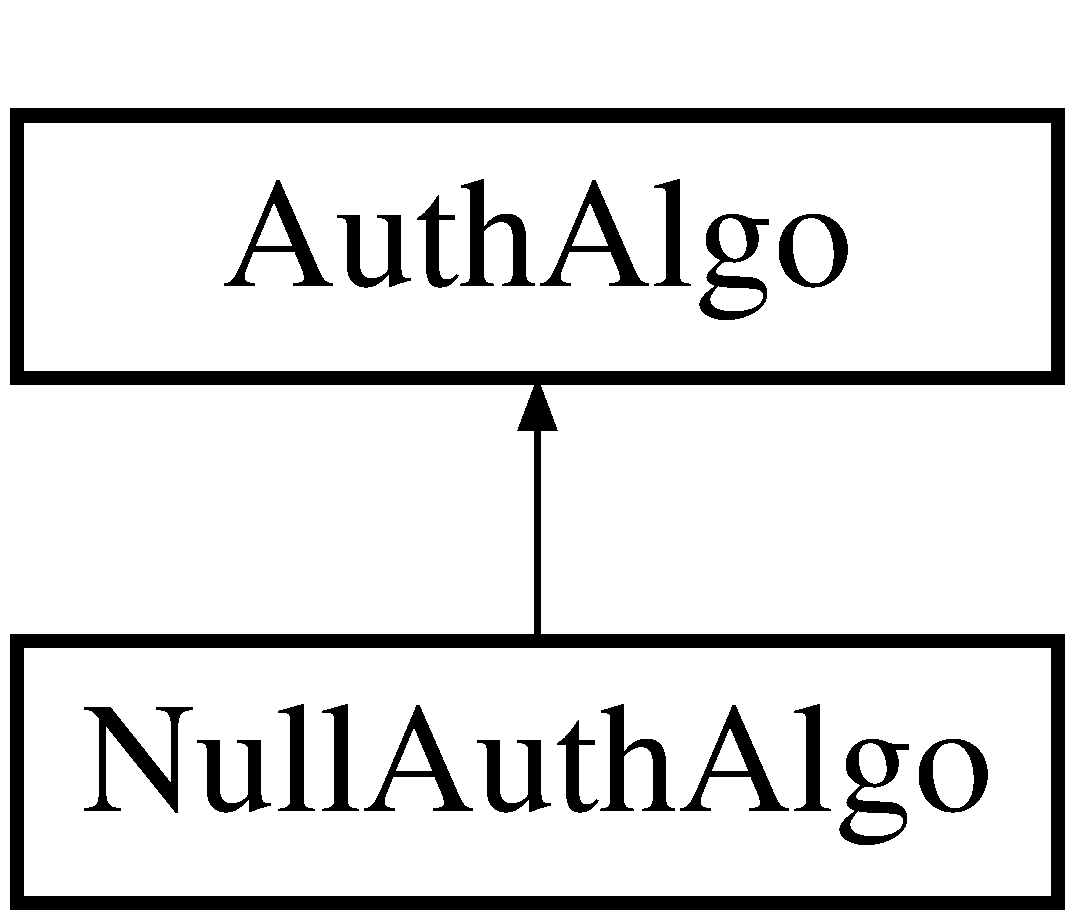
\includegraphics[height=2cm]{classNullAuthAlgo}
\end{center}
\end{figure}
\subsection*{Public Member Functions}
\begin{CompactItemize}
\item 
{\bf auth\_\-tag\_\-t} {\bf calc} (const {\bf Buffer} \&buf)
\end{CompactItemize}


\subsection{Member Function Documentation}
\index{NullAuthAlgo@{Null\-Auth\-Algo}!calc@{calc}}
\index{calc@{calc}!NullAuthAlgo@{Null\-Auth\-Algo}}
\subsubsection{\setlength{\rightskip}{0pt plus 5cm}{\bf auth\_\-tag\_\-t} Null\-Auth\-Algo::calc (const {\bf Buffer} \& {\em buf})\hspace{0.3cm}{\tt  [virtual]}}\label{classNullAuthAlgo_60eead12d6b32a576ad40d999a6151cf}




Implements {\bf Auth\-Algo} \doxyref{}{p.}{classAuthAlgo_f53b44f90c33eb049da260947a75c916}.

The documentation for this class was generated from the following files:\begin{CompactItemize}
\item 
{\bf auth\-Algo.h}\item 
{\bf auth\-Algo.cpp}\end{CompactItemize}

\section{Null\-Cypher Class Reference}
\label{classNullCypher}\index{NullCypher@{NullCypher}}
{\tt \#include $<$cypher.h$>$}

Inheritance diagram for Null\-Cypher::\begin{figure}[H]
\begin{center}
\leavevmode
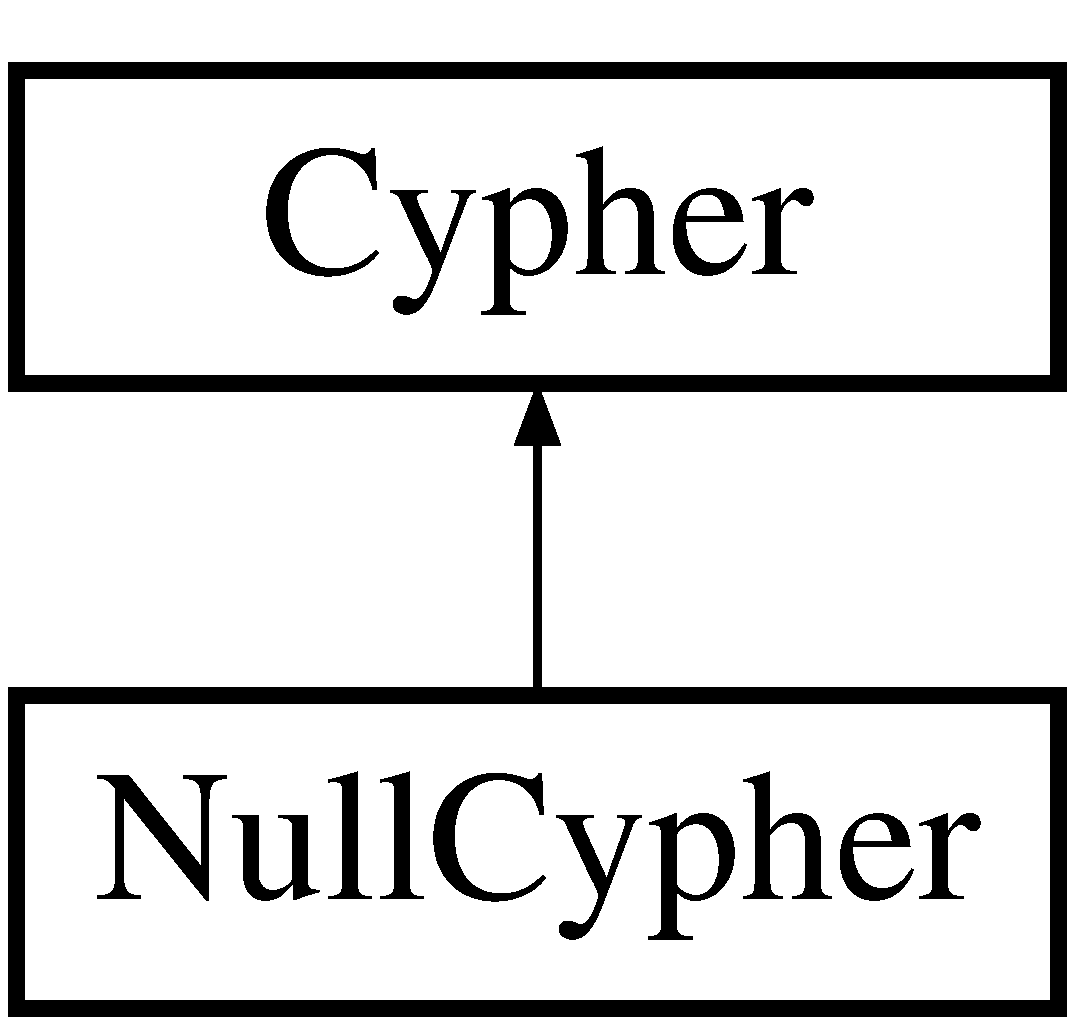
\includegraphics[height=2cm]{classNullCypher}
\end{center}
\end{figure}
\subsection*{Protected Member Functions}
\begin{CompactItemize}
\item 
{\bf Buffer} {\bf get\-Bit\-Stream} ({\bf u\_\-int32\_\-t} length, {\bf seq\_\-nr\_\-t} seq\_\-nr, {\bf sender\_\-id\_\-t} sender\_\-id)
\end{CompactItemize}


\subsection{Member Function Documentation}
\index{NullCypher@{Null\-Cypher}!getBitStream@{getBitStream}}
\index{getBitStream@{getBitStream}!NullCypher@{Null\-Cypher}}
\subsubsection{\setlength{\rightskip}{0pt plus 5cm}{\bf Buffer} Null\-Cypher::get\-Bit\-Stream ({\bf u\_\-int32\_\-t} {\em length}, {\bf seq\_\-nr\_\-t} {\em seq\_\-nr}, {\bf sender\_\-id\_\-t} {\em sender\_\-id})\hspace{0.3cm}{\tt  [protected, virtual]}}\label{classNullCypher_ca537adca8ea9af8b6f248df12ebcf36}




Implements {\bf Cypher} \doxyref{}{p.}{classCypher_7ddf1bcd476978daa97148ec406d6483}.

The documentation for this class was generated from the following files:\begin{CompactItemize}
\item 
{\bf cypher.h}\item 
{\bf cypher.cpp}\end{CompactItemize}

\section{Options Class Reference}
\label{classOptions}\index{Options@{Options}}
{\tt \#include $<$options.h$>$}

\subsection*{Public Member Functions}
\begin{CompactItemize}
\item 
{\bf Options} ()
\item 
bool {\bf parse} (int argc, char $\ast$argv[$\,$])
\item 
void {\bf print\-Usage} ()
\item 
void {\bf print\-Options} ()
\item 
std::string {\bf get\-Progname} ()
\item 
{\bf Options} \& {\bf set\-Progname} (std::string p)
\item 
{\bf sender\_\-id\_\-t} {\bf get\-Sender\-Id} ()
\item 
{\bf Options} \& {\bf set\-Sender\-Id} ({\bf sender\_\-id\_\-t} s)
\item 
std::string {\bf get\-Local\-Addr} ()
\item 
{\bf Options} \& {\bf set\-Local\-Addr} (std::string l)
\item 
{\bf u\_\-int16\_\-t} {\bf get\-Local\-Port} ()
\item 
{\bf Options} \& {\bf set\-Local\-Port} ({\bf u\_\-int16\_\-t} l)
\item 
std::string {\bf get\-Remote\-Addr} ()
\item 
{\bf Options} \& {\bf set\-Remote\-Addr} (std::string r)
\item 
{\bf u\_\-int16\_\-t} {\bf get\-Remote\-Port} ()
\item 
{\bf Options} \& {\bf set\-Remote\-Port} ({\bf u\_\-int16\_\-t} r)
\item 
{\bf Options} \& {\bf set\-Remote\-Addr\-Port} (std::string addr, {\bf u\_\-int16\_\-t} port)
\item 
std::string {\bf get\-Dev\-Name} ()
\item 
{\bf Options} \& {\bf set\-Dev\-Name} (std::string d)
\item 
std::string {\bf get\-Dev\-Type} ()
\item 
{\bf Options} \& {\bf set\-Dev\-Type} (std::string d)
\item 
std::string {\bf get\-Ifconfig\-Param\-Local} ()
\item 
{\bf Options} \& {\bf set\-Ifconfig\-Param\-Local} (std::string i)
\item 
std::string {\bf get\-Ifconfig\-Param\-Remote\-Netmask} ()
\item 
{\bf Options} \& {\bf set\-Ifconfig\-Param\-Remote\-Netmask} (std::string i)
\item 
{\bf window\_\-size\_\-t} {\bf get\-Seq\-Window\-Size} ()
\item 
{\bf Options} \& {\bf set\-Seq\-Window\-Size} ({\bf window\_\-size\_\-t} s)
\item 
std::string {\bf get\-Cypher} ()
\item 
{\bf Options} \& {\bf set\-Cypher} (std::string c)
\item 
std::string {\bf get\-Auth\-Algo} ()
\item 
{\bf Options} \& {\bf set\-Auth\-Algo} (std::string a)
\end{CompactItemize}
\subsection*{Private Attributes}
\begin{CompactItemize}
\item 
{\bf Mutex} {\bf mutex}
\item 
std::string {\bf progname\_\-}
\item 
{\bf sender\_\-id\_\-t} {\bf sender\_\-id\_\-}
\item 
std::string {\bf local\_\-addr\_\-}
\item 
{\bf u\_\-int16\_\-t} {\bf local\_\-port\_\-}
\item 
std::string {\bf remote\_\-addr\_\-}
\item 
{\bf u\_\-int16\_\-t} {\bf remote\_\-port\_\-}
\item 
std::string {\bf dev\_\-name\_\-}
\item 
std::string {\bf dev\_\-type\_\-}
\item 
std::string {\bf ifconfig\_\-param\_\-local\_\-}
\item 
std::string {\bf ifconfig\_\-param\_\-remote\_\-netmask\_\-}
\item 
{\bf window\_\-size\_\-t} {\bf seq\_\-window\_\-size\_\-}
\item 
std::string {\bf cypher\_\-}
\item 
std::string {\bf auth\_\-algo\_\-}
\end{CompactItemize}


\subsection{Constructor \& Destructor Documentation}
\index{Options@{Options}!Options@{Options}}
\index{Options@{Options}!Options@{Options}}
\subsubsection{\setlength{\rightskip}{0pt plus 5cm}Options::Options ()}\label{classOptions_b72fb640172a6109e34c8a5366563753}




\subsection{Member Function Documentation}
\index{Options@{Options}!parse@{parse}}
\index{parse@{parse}!Options@{Options}}
\subsubsection{\setlength{\rightskip}{0pt plus 5cm}bool Options::parse (int {\em argc}, char $\ast$ {\em argv}[$\,$])}\label{classOptions_eef7f9799ffcc31221a54dc9ed3b3e81}


\index{Options@{Options}!printUsage@{printUsage}}
\index{printUsage@{printUsage}!Options@{Options}}
\subsubsection{\setlength{\rightskip}{0pt plus 5cm}void Options::print\-Usage ()}\label{classOptions_5a64af47966f3c0a54a8c3a3385065e3}


\index{Options@{Options}!printOptions@{printOptions}}
\index{printOptions@{printOptions}!Options@{Options}}
\subsubsection{\setlength{\rightskip}{0pt plus 5cm}void Options::print\-Options ()}\label{classOptions_cac40a32d05b48e49595d8d19cf8af47}


\index{Options@{Options}!getProgname@{getProgname}}
\index{getProgname@{getProgname}!Options@{Options}}
\subsubsection{\setlength{\rightskip}{0pt plus 5cm}std::string Options::get\-Progname ()}\label{classOptions_af7b2ab27fc4b1a74ef89e9fdd0cfb22}


\index{Options@{Options}!setProgname@{setProgname}}
\index{setProgname@{setProgname}!Options@{Options}}
\subsubsection{\setlength{\rightskip}{0pt plus 5cm}{\bf Options} \& Options::set\-Progname (std::string {\em p})}\label{classOptions_1267ce6d4b43ab9c0f8827c434b33b1b}


\index{Options@{Options}!getSenderId@{getSenderId}}
\index{getSenderId@{getSenderId}!Options@{Options}}
\subsubsection{\setlength{\rightskip}{0pt plus 5cm}{\bf sender\_\-id\_\-t} Options::get\-Sender\-Id ()}\label{classOptions_049d0dbe0f6ca10cc18d87924fb2322d}


\index{Options@{Options}!setSenderId@{setSenderId}}
\index{setSenderId@{setSenderId}!Options@{Options}}
\subsubsection{\setlength{\rightskip}{0pt plus 5cm}{\bf Options} \& Options::set\-Sender\-Id ({\bf sender\_\-id\_\-t} {\em s})}\label{classOptions_d10f65b29130c7e31a332e22f77650b0}


\index{Options@{Options}!getLocalAddr@{getLocalAddr}}
\index{getLocalAddr@{getLocalAddr}!Options@{Options}}
\subsubsection{\setlength{\rightskip}{0pt plus 5cm}std::string Options::get\-Local\-Addr ()}\label{classOptions_0b1ca05363913a66db8dcb829ebc21e2}


\index{Options@{Options}!setLocalAddr@{setLocalAddr}}
\index{setLocalAddr@{setLocalAddr}!Options@{Options}}
\subsubsection{\setlength{\rightskip}{0pt plus 5cm}{\bf Options} \& Options::set\-Local\-Addr (std::string {\em l})}\label{classOptions_bf7ebb3ee98c6d31dd5c5b0732188de5}


\index{Options@{Options}!getLocalPort@{getLocalPort}}
\index{getLocalPort@{getLocalPort}!Options@{Options}}
\subsubsection{\setlength{\rightskip}{0pt plus 5cm}{\bf u\_\-int16\_\-t} Options::get\-Local\-Port ()}\label{classOptions_44a66c61b99fc0d1a953493a3cd4dcab}


\index{Options@{Options}!setLocalPort@{setLocalPort}}
\index{setLocalPort@{setLocalPort}!Options@{Options}}
\subsubsection{\setlength{\rightskip}{0pt plus 5cm}{\bf Options} \& Options::set\-Local\-Port ({\bf u\_\-int16\_\-t} {\em l})}\label{classOptions_a4b5b364bf2880fcbcd3fe059ccde7eb}


\index{Options@{Options}!getRemoteAddr@{getRemoteAddr}}
\index{getRemoteAddr@{getRemoteAddr}!Options@{Options}}
\subsubsection{\setlength{\rightskip}{0pt plus 5cm}std::string Options::get\-Remote\-Addr ()}\label{classOptions_46343d900b4dd2ab8e0a7a2a9274e885}


\index{Options@{Options}!setRemoteAddr@{setRemoteAddr}}
\index{setRemoteAddr@{setRemoteAddr}!Options@{Options}}
\subsubsection{\setlength{\rightskip}{0pt plus 5cm}{\bf Options} \& Options::set\-Remote\-Addr (std::string {\em r})}\label{classOptions_d0848af5b5e029a4ea14fe6fb82d3f46}


\index{Options@{Options}!getRemotePort@{getRemotePort}}
\index{getRemotePort@{getRemotePort}!Options@{Options}}
\subsubsection{\setlength{\rightskip}{0pt plus 5cm}{\bf u\_\-int16\_\-t} Options::get\-Remote\-Port ()}\label{classOptions_4d2089d4216557810410f31ffa2dfc8b}


\index{Options@{Options}!setRemotePort@{setRemotePort}}
\index{setRemotePort@{setRemotePort}!Options@{Options}}
\subsubsection{\setlength{\rightskip}{0pt plus 5cm}{\bf Options} \& Options::set\-Remote\-Port ({\bf u\_\-int16\_\-t} {\em r})}\label{classOptions_cbd3e9a4e230c2537d86127a092efd40}


\index{Options@{Options}!setRemoteAddrPort@{setRemoteAddrPort}}
\index{setRemoteAddrPort@{setRemoteAddrPort}!Options@{Options}}
\subsubsection{\setlength{\rightskip}{0pt plus 5cm}{\bf Options} \& Options::set\-Remote\-Addr\-Port (std::string {\em addr}, {\bf u\_\-int16\_\-t} {\em port})}\label{classOptions_79249268d3b284f9e254f874cedeef41}


\index{Options@{Options}!getDevName@{getDevName}}
\index{getDevName@{getDevName}!Options@{Options}}
\subsubsection{\setlength{\rightskip}{0pt plus 5cm}std::string Options::get\-Dev\-Name ()}\label{classOptions_acd35d4f958a4611ba10fc844583b744}


\index{Options@{Options}!setDevName@{setDevName}}
\index{setDevName@{setDevName}!Options@{Options}}
\subsubsection{\setlength{\rightskip}{0pt plus 5cm}{\bf Options} \& Options::set\-Dev\-Name (std::string {\em d})}\label{classOptions_8217facd595355be2b4f1130179e3746}


\index{Options@{Options}!getDevType@{getDevType}}
\index{getDevType@{getDevType}!Options@{Options}}
\subsubsection{\setlength{\rightskip}{0pt plus 5cm}std::string Options::get\-Dev\-Type ()}\label{classOptions_0762384e71fb10883a8fe245a389cee6}


\index{Options@{Options}!setDevType@{setDevType}}
\index{setDevType@{setDevType}!Options@{Options}}
\subsubsection{\setlength{\rightskip}{0pt plus 5cm}{\bf Options} \& Options::set\-Dev\-Type (std::string {\em d})}\label{classOptions_d2a4cc3b2ecabba72396648a7a07cc29}


\index{Options@{Options}!getIfconfigParamLocal@{getIfconfigParamLocal}}
\index{getIfconfigParamLocal@{getIfconfigParamLocal}!Options@{Options}}
\subsubsection{\setlength{\rightskip}{0pt plus 5cm}std::string Options::get\-Ifconfig\-Param\-Local ()}\label{classOptions_5354b737aa30d786c79f43547c78dc09}


\index{Options@{Options}!setIfconfigParamLocal@{setIfconfigParamLocal}}
\index{setIfconfigParamLocal@{setIfconfigParamLocal}!Options@{Options}}
\subsubsection{\setlength{\rightskip}{0pt plus 5cm}{\bf Options} \& Options::set\-Ifconfig\-Param\-Local (std::string {\em i})}\label{classOptions_93e1367e5db67df81d2afac1ee5c6c73}


\index{Options@{Options}!getIfconfigParamRemoteNetmask@{getIfconfigParamRemoteNetmask}}
\index{getIfconfigParamRemoteNetmask@{getIfconfigParamRemoteNetmask}!Options@{Options}}
\subsubsection{\setlength{\rightskip}{0pt plus 5cm}std::string Options::get\-Ifconfig\-Param\-Remote\-Netmask ()}\label{classOptions_ee9e8bcc21c6c8c81fc4ed79991d42d5}


\index{Options@{Options}!setIfconfigParamRemoteNetmask@{setIfconfigParamRemoteNetmask}}
\index{setIfconfigParamRemoteNetmask@{setIfconfigParamRemoteNetmask}!Options@{Options}}
\subsubsection{\setlength{\rightskip}{0pt plus 5cm}{\bf Options} \& Options::set\-Ifconfig\-Param\-Remote\-Netmask (std::string {\em i})}\label{classOptions_d0760cecce7395f5022b921642674326}


\index{Options@{Options}!getSeqWindowSize@{getSeqWindowSize}}
\index{getSeqWindowSize@{getSeqWindowSize}!Options@{Options}}
\subsubsection{\setlength{\rightskip}{0pt plus 5cm}{\bf window\_\-size\_\-t} Options::get\-Seq\-Window\-Size ()}\label{classOptions_893c688302a091bcf99cb327b23774fa}


\index{Options@{Options}!setSeqWindowSize@{setSeqWindowSize}}
\index{setSeqWindowSize@{setSeqWindowSize}!Options@{Options}}
\subsubsection{\setlength{\rightskip}{0pt plus 5cm}{\bf Options} \& Options::set\-Seq\-Window\-Size ({\bf window\_\-size\_\-t} {\em s})}\label{classOptions_077dda754c64b01d6736aa4f7862ce6b}


\index{Options@{Options}!getCypher@{getCypher}}
\index{getCypher@{getCypher}!Options@{Options}}
\subsubsection{\setlength{\rightskip}{0pt plus 5cm}std::string Options::get\-Cypher ()}\label{classOptions_71845d106fb9ccef0f8b682a125f4ffd}


\index{Options@{Options}!setCypher@{setCypher}}
\index{setCypher@{setCypher}!Options@{Options}}
\subsubsection{\setlength{\rightskip}{0pt plus 5cm}{\bf Options} \& Options::set\-Cypher (std::string {\em c})}\label{classOptions_b3218cd91b41551042595b5216766c00}


\index{Options@{Options}!getAuthAlgo@{getAuthAlgo}}
\index{getAuthAlgo@{getAuthAlgo}!Options@{Options}}
\subsubsection{\setlength{\rightskip}{0pt plus 5cm}std::string Options::get\-Auth\-Algo ()}\label{classOptions_ee7bd7127b7ab35e287fb479288e9641}


\index{Options@{Options}!setAuthAlgo@{setAuthAlgo}}
\index{setAuthAlgo@{setAuthAlgo}!Options@{Options}}
\subsubsection{\setlength{\rightskip}{0pt plus 5cm}{\bf Options} \& Options::set\-Auth\-Algo (std::string {\em a})}\label{classOptions_c093c83be9a50c1dfd5170ff14b647c5}




\subsection{Member Data Documentation}
\index{Options@{Options}!mutex@{mutex}}
\index{mutex@{mutex}!Options@{Options}}
\subsubsection{\setlength{\rightskip}{0pt plus 5cm}{\bf Mutex} {\bf Options::mutex}\hspace{0.3cm}{\tt  [private]}}\label{classOptions_3effd9220086fd43e36884295f89bd7c}


\index{Options@{Options}!progname_@{progname\_\-}}
\index{progname_@{progname\_\-}!Options@{Options}}
\subsubsection{\setlength{\rightskip}{0pt plus 5cm}std::string {\bf Options::progname\_\-}\hspace{0.3cm}{\tt  [private]}}\label{classOptions_aed7d0eeae21d7d00eb35dccea48b9f3}


\index{Options@{Options}!sender_id_@{sender\_\-id\_\-}}
\index{sender_id_@{sender\_\-id\_\-}!Options@{Options}}
\subsubsection{\setlength{\rightskip}{0pt plus 5cm}{\bf sender\_\-id\_\-t} {\bf Options::sender\_\-id\_\-}\hspace{0.3cm}{\tt  [private]}}\label{classOptions_f166d5f4f6fd17c761ac9a6d7e48d362}


\index{Options@{Options}!local_addr_@{local\_\-addr\_\-}}
\index{local_addr_@{local\_\-addr\_\-}!Options@{Options}}
\subsubsection{\setlength{\rightskip}{0pt plus 5cm}std::string {\bf Options::local\_\-addr\_\-}\hspace{0.3cm}{\tt  [private]}}\label{classOptions_d331507d07c87908a5b199a209a3e97e}


\index{Options@{Options}!local_port_@{local\_\-port\_\-}}
\index{local_port_@{local\_\-port\_\-}!Options@{Options}}
\subsubsection{\setlength{\rightskip}{0pt plus 5cm}{\bf u\_\-int16\_\-t} {\bf Options::local\_\-port\_\-}\hspace{0.3cm}{\tt  [private]}}\label{classOptions_744fc32e1b4f5c930251a8b0013f7f0a}


\index{Options@{Options}!remote_addr_@{remote\_\-addr\_\-}}
\index{remote_addr_@{remote\_\-addr\_\-}!Options@{Options}}
\subsubsection{\setlength{\rightskip}{0pt plus 5cm}std::string {\bf Options::remote\_\-addr\_\-}\hspace{0.3cm}{\tt  [private]}}\label{classOptions_af81d4d836e3ca1850b8b474d61944de}


\index{Options@{Options}!remote_port_@{remote\_\-port\_\-}}
\index{remote_port_@{remote\_\-port\_\-}!Options@{Options}}
\subsubsection{\setlength{\rightskip}{0pt plus 5cm}{\bf u\_\-int16\_\-t} {\bf Options::remote\_\-port\_\-}\hspace{0.3cm}{\tt  [private]}}\label{classOptions_8481cdc79ca8bde93af9b945838f4559}


\index{Options@{Options}!dev_name_@{dev\_\-name\_\-}}
\index{dev_name_@{dev\_\-name\_\-}!Options@{Options}}
\subsubsection{\setlength{\rightskip}{0pt plus 5cm}std::string {\bf Options::dev\_\-name\_\-}\hspace{0.3cm}{\tt  [private]}}\label{classOptions_3b094d71270549c85ca372f060bfe22c}


\index{Options@{Options}!dev_type_@{dev\_\-type\_\-}}
\index{dev_type_@{dev\_\-type\_\-}!Options@{Options}}
\subsubsection{\setlength{\rightskip}{0pt plus 5cm}std::string {\bf Options::dev\_\-type\_\-}\hspace{0.3cm}{\tt  [private]}}\label{classOptions_b0c850a5e29599156af92cf5b3ddff28}


\index{Options@{Options}!ifconfig_param_local_@{ifconfig\_\-param\_\-local\_\-}}
\index{ifconfig_param_local_@{ifconfig\_\-param\_\-local\_\-}!Options@{Options}}
\subsubsection{\setlength{\rightskip}{0pt plus 5cm}std::string {\bf Options::ifconfig\_\-param\_\-local\_\-}\hspace{0.3cm}{\tt  [private]}}\label{classOptions_fd0d76c7e1e2fa6fd9ee0538ff9124b0}


\index{Options@{Options}!ifconfig_param_remote_netmask_@{ifconfig\_\-param\_\-remote\_\-netmask\_\-}}
\index{ifconfig_param_remote_netmask_@{ifconfig\_\-param\_\-remote\_\-netmask\_\-}!Options@{Options}}
\subsubsection{\setlength{\rightskip}{0pt plus 5cm}std::string {\bf Options::ifconfig\_\-param\_\-remote\_\-netmask\_\-}\hspace{0.3cm}{\tt  [private]}}\label{classOptions_cd2c34152754ab7818ee4bfe3e1b9936}


\index{Options@{Options}!seq_window_size_@{seq\_\-window\_\-size\_\-}}
\index{seq_window_size_@{seq\_\-window\_\-size\_\-}!Options@{Options}}
\subsubsection{\setlength{\rightskip}{0pt plus 5cm}{\bf window\_\-size\_\-t} {\bf Options::seq\_\-window\_\-size\_\-}\hspace{0.3cm}{\tt  [private]}}\label{classOptions_d2a0398f717a96602f8c402db12699a5}


\index{Options@{Options}!cypher_@{cypher\_\-}}
\index{cypher_@{cypher\_\-}!Options@{Options}}
\subsubsection{\setlength{\rightskip}{0pt plus 5cm}std::string {\bf Options::cypher\_\-}\hspace{0.3cm}{\tt  [private]}}\label{classOptions_bba16365a15a6a87c90f85e143bebb5f}


\index{Options@{Options}!auth_algo_@{auth\_\-algo\_\-}}
\index{auth_algo_@{auth\_\-algo\_\-}!Options@{Options}}
\subsubsection{\setlength{\rightskip}{0pt plus 5cm}std::string {\bf Options::auth\_\-algo\_\-}\hspace{0.3cm}{\tt  [private]}}\label{classOptions_061ed690bdfa12bfc1094ca18293e97a}




The documentation for this class was generated from the following files:\begin{CompactItemize}
\item 
{\bf options.h}\item 
{\bf options.cpp}\end{CompactItemize}

\section{Packet Class Reference}
\label{classPacket}\index{Packet@{Packet}}
{\tt \#include $<$packet.h$>$}

Inheritance diagram for Packet::\begin{figure}[H]
\begin{center}
\leavevmode
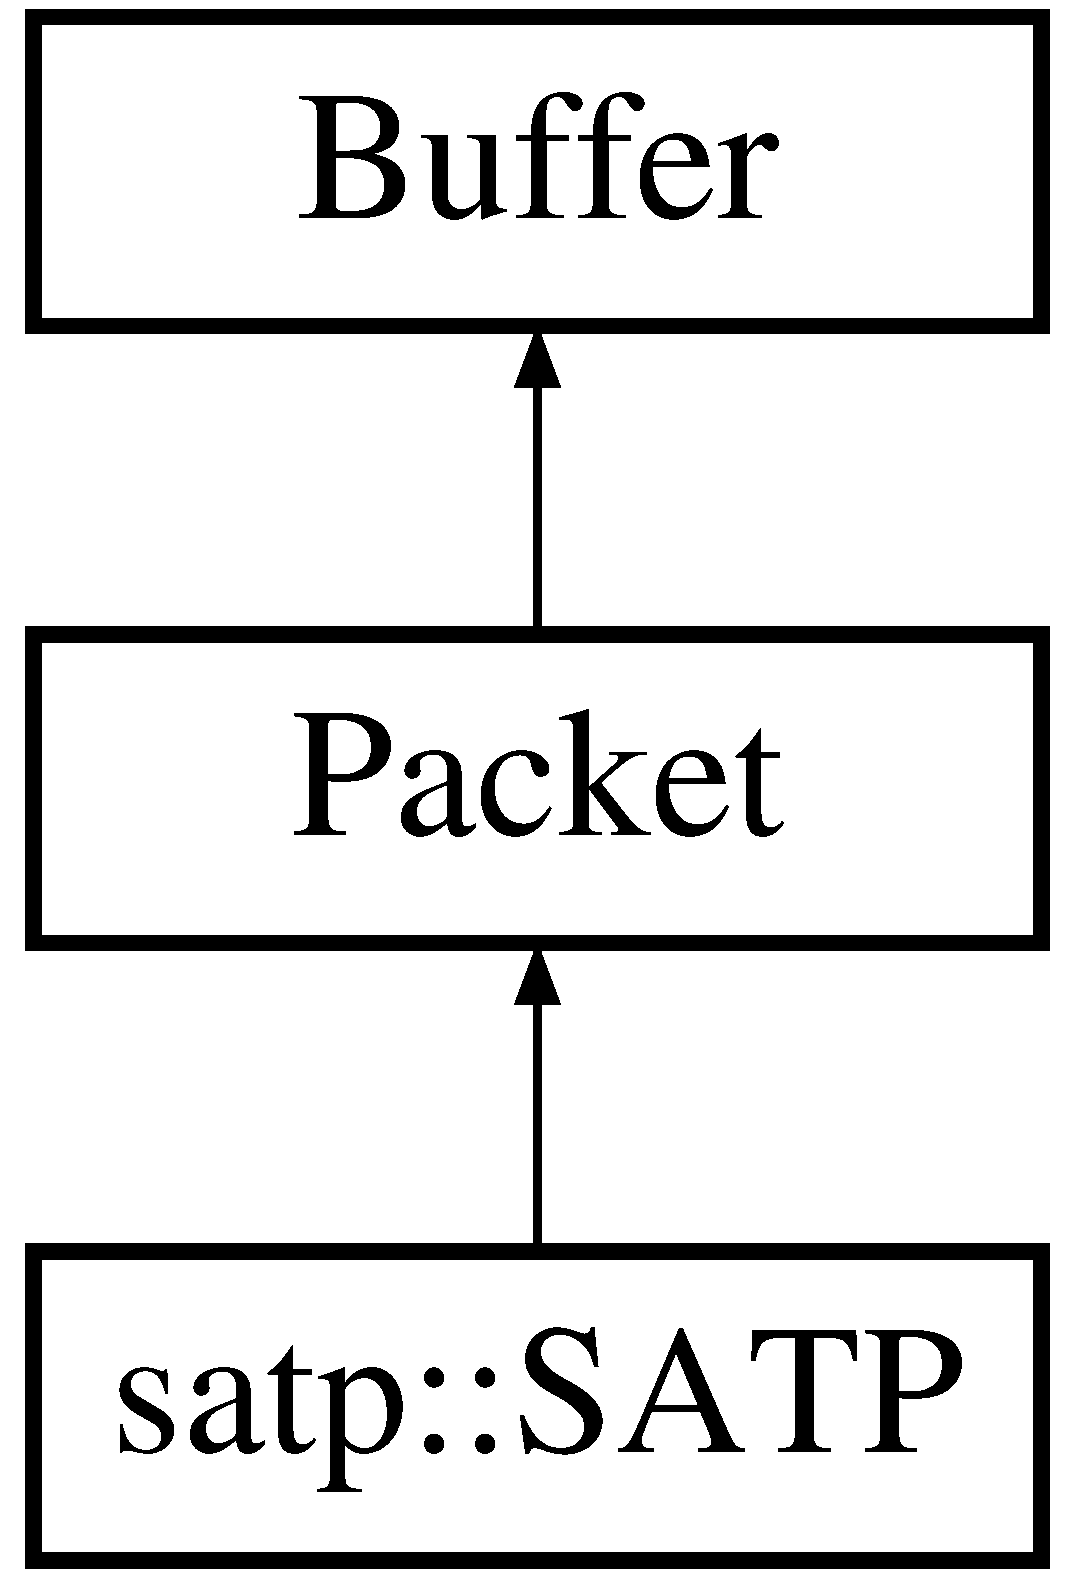
\includegraphics[height=3cm]{classPacket}
\end{center}
\end{figure}
\subsection*{Public Member Functions}
\begin{CompactItemize}
\item 
{\bf Packet} ()
\item 
{\bf Packet} ({\bf u\_\-int32\_\-t} length)
\item 
{\bf Packet} (const {\bf Buffer} \&src)
\item 
bool {\bf has\-Header} () const
\item 
{\bf Packet} \& {\bf with\-Header} (bool b)
\item 
{\bf seq\_\-nr\_\-t} {\bf get\-Seq\-Nr} () const
\item 
{\bf sender\_\-id\_\-t} {\bf get\-Sender\-Id} () const
\item 
{\bf Packet} \& {\bf add\-Header} ({\bf seq\_\-nr\_\-t} seq\_\-nr, {\bf sender\_\-id\_\-t} sender\_\-id)
\item 
{\bf Packet} \& {\bf remove\-Header} ()
\item 
{\bf Packet} \& {\bf set\-Seq\-Nr} ({\bf seq\_\-nr\_\-t} seq\_\-nr)
\item 
{\bf Packet} \& {\bf set\-Sender\-Id} ({\bf sender\_\-id\_\-t} sender\_\-id)
\item 
bool {\bf has\-Payload\-Type} () const
\item 
{\bf Packet} \& {\bf with\-Payload\-Type} (bool b)
\item 
{\bf payload\_\-type\_\-t} {\bf get\-Payload\-Type} () const
\item 
{\bf Packet} \& {\bf add\-Payload\-Type} ({\bf payload\_\-type\_\-t} payload\_\-type)
\item 
{\bf Packet} \& {\bf remove\-Payload\-Type} ()
\item 
bool {\bf has\-Auth\-Tag} () const
\item 
{\bf Packet} \& {\bf with\-Auth\-Tag} (bool b)
\item 
{\bf auth\_\-tag\_\-t} {\bf get\-Auth\-Tag} () const
\item 
{\bf Packet} \& {\bf add\-Auth\-Tag} ({\bf auth\_\-tag\_\-t} auth\_\-tag)
\item 
{\bf Packet} \& {\bf remove\-Auth\-Tag} ()
\end{CompactItemize}
\subsection*{Private Attributes}
\begin{CompactItemize}
\item 
{\bf Packet::Header\-Struct} {\bf \_\-\_\-packed\_\-\_\-}
\item 
bool {\bf has\_\-header\_\-}
\item 
bool {\bf has\_\-payload\_\-type\_\-}
\item 
bool {\bf has\_\-auth\_\-tag\_\-}
\end{CompactItemize}
\subsection*{Classes}
\begin{CompactItemize}
\item 
struct {\bf Header\-Struct}
\end{CompactItemize}


\subsection{Constructor \& Destructor Documentation}
\index{Packet@{Packet}!Packet@{Packet}}
\index{Packet@{Packet}!Packet@{Packet}}
\subsubsection{\setlength{\rightskip}{0pt plus 5cm}Packet::Packet ()}\label{classPacket_abcfb963c0d5bc0fa554668f92989622}


\index{Packet@{Packet}!Packet@{Packet}}
\index{Packet@{Packet}!Packet@{Packet}}
\subsubsection{\setlength{\rightskip}{0pt plus 5cm}Packet::Packet ({\bf u\_\-int32\_\-t} {\em length})}\label{classPacket_d2a8f6ac3d6de9b541708c4b0c73d04b}


\index{Packet@{Packet}!Packet@{Packet}}
\index{Packet@{Packet}!Packet@{Packet}}
\subsubsection{\setlength{\rightskip}{0pt plus 5cm}Packet::Packet (const {\bf Buffer} \& {\em src})}\label{classPacket_27264b7d411a74ea9a0077bf5f9222b1}




\subsection{Member Function Documentation}
\index{Packet@{Packet}!hasHeader@{hasHeader}}
\index{hasHeader@{hasHeader}!Packet@{Packet}}
\subsubsection{\setlength{\rightskip}{0pt plus 5cm}bool Packet::has\-Header () const}\label{classPacket_a004c01dd99179b0a08109dce5fc6b03}


\index{Packet@{Packet}!withHeader@{withHeader}}
\index{withHeader@{withHeader}!Packet@{Packet}}
\subsubsection{\setlength{\rightskip}{0pt plus 5cm}{\bf Packet} \& Packet::with\-Header (bool {\em b})}\label{classPacket_ce9e40180f64d44fe1d8da14ac9e5df2}


\index{Packet@{Packet}!getSeqNr@{getSeqNr}}
\index{getSeqNr@{getSeqNr}!Packet@{Packet}}
\subsubsection{\setlength{\rightskip}{0pt plus 5cm}{\bf seq\_\-nr\_\-t} Packet::get\-Seq\-Nr () const}\label{classPacket_6572b9df8c1f5f0de9fcb8e5c669de50}


\index{Packet@{Packet}!getSenderId@{getSenderId}}
\index{getSenderId@{getSenderId}!Packet@{Packet}}
\subsubsection{\setlength{\rightskip}{0pt plus 5cm}{\bf sender\_\-id\_\-t} Packet::get\-Sender\-Id () const}\label{classPacket_096829acfcf98c3ffff60bd335cbb919}


\index{Packet@{Packet}!addHeader@{addHeader}}
\index{addHeader@{addHeader}!Packet@{Packet}}
\subsubsection{\setlength{\rightskip}{0pt plus 5cm}{\bf Packet} \& Packet::add\-Header ({\bf seq\_\-nr\_\-t} {\em seq\_\-nr}, {\bf sender\_\-id\_\-t} {\em sender\_\-id})}\label{classPacket_2a682115c6802d0dd1ebbd3434a3a179}


\index{Packet@{Packet}!removeHeader@{removeHeader}}
\index{removeHeader@{removeHeader}!Packet@{Packet}}
\subsubsection{\setlength{\rightskip}{0pt plus 5cm}{\bf Packet} \& Packet::remove\-Header ()}\label{classPacket_24c2a41630d79411086d952c8f732c8c}


\index{Packet@{Packet}!setSeqNr@{setSeqNr}}
\index{setSeqNr@{setSeqNr}!Packet@{Packet}}
\subsubsection{\setlength{\rightskip}{0pt plus 5cm}{\bf Packet} \& Packet::set\-Seq\-Nr ({\bf seq\_\-nr\_\-t} {\em seq\_\-nr})}\label{classPacket_1b89ed1be19d6b9c1a12e0f6b1ae8ed2}


\index{Packet@{Packet}!setSenderId@{setSenderId}}
\index{setSenderId@{setSenderId}!Packet@{Packet}}
\subsubsection{\setlength{\rightskip}{0pt plus 5cm}{\bf Packet} \& Packet::set\-Sender\-Id ({\bf sender\_\-id\_\-t} {\em sender\_\-id})}\label{classPacket_01c7b848ec415740565c87b374085bdc}


\index{Packet@{Packet}!hasPayloadType@{hasPayloadType}}
\index{hasPayloadType@{hasPayloadType}!Packet@{Packet}}
\subsubsection{\setlength{\rightskip}{0pt plus 5cm}bool Packet::has\-Payload\-Type () const}\label{classPacket_c78b8af0dc7c7badf85e75db0de54800}


\index{Packet@{Packet}!withPayloadType@{withPayloadType}}
\index{withPayloadType@{withPayloadType}!Packet@{Packet}}
\subsubsection{\setlength{\rightskip}{0pt plus 5cm}{\bf Packet} \& Packet::with\-Payload\-Type (bool {\em b})}\label{classPacket_c7ecfc05376afd00af89cb328e194a1d}


\index{Packet@{Packet}!getPayloadType@{getPayloadType}}
\index{getPayloadType@{getPayloadType}!Packet@{Packet}}
\subsubsection{\setlength{\rightskip}{0pt plus 5cm}{\bf payload\_\-type\_\-t} Packet::get\-Payload\-Type () const}\label{classPacket_ed7f5cc79b40a11eddefd4b421544498}


\index{Packet@{Packet}!addPayloadType@{addPayloadType}}
\index{addPayloadType@{addPayloadType}!Packet@{Packet}}
\subsubsection{\setlength{\rightskip}{0pt plus 5cm}{\bf Packet} \& Packet::add\-Payload\-Type ({\bf payload\_\-type\_\-t} {\em payload\_\-type})}\label{classPacket_40849ee3c59a84c3899c409ed392b477}


\index{Packet@{Packet}!removePayloadType@{removePayloadType}}
\index{removePayloadType@{removePayloadType}!Packet@{Packet}}
\subsubsection{\setlength{\rightskip}{0pt plus 5cm}{\bf Packet} \& Packet::remove\-Payload\-Type ()}\label{classPacket_6433e4d5eef9216f4e70b338cb4d2e4d}


\index{Packet@{Packet}!hasAuthTag@{hasAuthTag}}
\index{hasAuthTag@{hasAuthTag}!Packet@{Packet}}
\subsubsection{\setlength{\rightskip}{0pt plus 5cm}bool Packet::has\-Auth\-Tag () const}\label{classPacket_bfe50722f18687bb0691061fb0ccb0ff}


\index{Packet@{Packet}!withAuthTag@{withAuthTag}}
\index{withAuthTag@{withAuthTag}!Packet@{Packet}}
\subsubsection{\setlength{\rightskip}{0pt plus 5cm}{\bf Packet} \& Packet::with\-Auth\-Tag (bool {\em b})}\label{classPacket_5c947adee9eef0a662a4dc49d95dbe8e}


\index{Packet@{Packet}!getAuthTag@{getAuthTag}}
\index{getAuthTag@{getAuthTag}!Packet@{Packet}}
\subsubsection{\setlength{\rightskip}{0pt plus 5cm}{\bf auth\_\-tag\_\-t} Packet::get\-Auth\-Tag () const}\label{classPacket_ba55c639065c177a7006d8392f50eddc}


\index{Packet@{Packet}!addAuthTag@{addAuthTag}}
\index{addAuthTag@{addAuthTag}!Packet@{Packet}}
\subsubsection{\setlength{\rightskip}{0pt plus 5cm}{\bf Packet} \& Packet::add\-Auth\-Tag ({\bf auth\_\-tag\_\-t} {\em auth\_\-tag})}\label{classPacket_a7f8bb4bb127aad314eb0f0ef72447ed}


\index{Packet@{Packet}!removeAuthTag@{removeAuthTag}}
\index{removeAuthTag@{removeAuthTag}!Packet@{Packet}}
\subsubsection{\setlength{\rightskip}{0pt plus 5cm}{\bf Packet} \& Packet::remove\-Auth\-Tag ()}\label{classPacket_3e3dfca708baf59791f0608b8a57924c}




\subsection{Member Data Documentation}
\index{Packet@{Packet}!__packed__@{\_\-\_\-packed\_\-\_\-}}
\index{__packed__@{\_\-\_\-packed\_\-\_\-}!Packet@{Packet}}
\subsubsection{\setlength{\rightskip}{0pt plus 5cm}struct {\bf Packet::Header\-Struct} {\bf Packet::\_\-\_\-packed\_\-\_\-}\hspace{0.3cm}{\tt  [private]}}\label{classPacket_11b3534f67df6bb19963e6bc8090230b}


\index{Packet@{Packet}!has_header_@{has\_\-header\_\-}}
\index{has_header_@{has\_\-header\_\-}!Packet@{Packet}}
\subsubsection{\setlength{\rightskip}{0pt plus 5cm}bool {\bf Packet::has\_\-header\_\-}\hspace{0.3cm}{\tt  [private]}}\label{classPacket_97b8eb52e7476174a0e91e2ccaf73306}


\index{Packet@{Packet}!has_payload_type_@{has\_\-payload\_\-type\_\-}}
\index{has_payload_type_@{has\_\-payload\_\-type\_\-}!Packet@{Packet}}
\subsubsection{\setlength{\rightskip}{0pt plus 5cm}bool {\bf Packet::has\_\-payload\_\-type\_\-}\hspace{0.3cm}{\tt  [private]}}\label{classPacket_235c6c8c7362c46ca33a331713199a17}


\index{Packet@{Packet}!has_auth_tag_@{has\_\-auth\_\-tag\_\-}}
\index{has_auth_tag_@{has\_\-auth\_\-tag\_\-}!Packet@{Packet}}
\subsubsection{\setlength{\rightskip}{0pt plus 5cm}bool {\bf Packet::has\_\-auth\_\-tag\_\-}\hspace{0.3cm}{\tt  [private]}}\label{classPacket_849a965c46afc5fa7efe257212197abb}




The documentation for this class was generated from the following files:\begin{CompactItemize}
\item 
{\bf packet.h}\item 
{\bf packet.cpp}\end{CompactItemize}

\section{Packet::Header\-Struct Struct Reference}
\label{structPacket_1_1HeaderStruct}\index{Packet::HeaderStruct@{Packet::HeaderStruct}}
\subsection*{Public Attributes}
\begin{CompactItemize}
\item 
{\bf seq\_\-nr\_\-t} {\bf seq\_\-nr}
\item 
{\bf sender\_\-id\_\-t} {\bf sender\_\-id}
\end{CompactItemize}


\subsection{Member Data Documentation}
\index{Packet::HeaderStruct@{Packet::Header\-Struct}!seq_nr@{seq\_\-nr}}
\index{seq_nr@{seq\_\-nr}!Packet::HeaderStruct@{Packet::Header\-Struct}}
\subsubsection{\setlength{\rightskip}{0pt plus 5cm}{\bf seq\_\-nr\_\-t} {\bf Packet::Header\-Struct::seq\_\-nr}}\label{structPacket_1_1HeaderStruct_4b7b9bf68b204ca98171b7f818685521}


\index{Packet::HeaderStruct@{Packet::Header\-Struct}!sender_id@{sender\_\-id}}
\index{sender_id@{sender\_\-id}!Packet::HeaderStruct@{Packet::Header\-Struct}}
\subsubsection{\setlength{\rightskip}{0pt plus 5cm}{\bf sender\_\-id\_\-t} {\bf Packet::Header\-Struct::sender\_\-id}}\label{structPacket_1_1HeaderStruct_c129b7cda1d848a579b689bacdabddea}




The documentation for this struct was generated from the following file:\begin{CompactItemize}
\item 
{\bf packet.h}\end{CompactItemize}

\section{Packet\-Source Class Reference}
\label{classPacketSource}\index{PacketSource@{PacketSource}}
{\tt \#include $<$packet\-Source.h$>$}

Inheritance diagram for Packet\-Source::\begin{figure}[H]
\begin{center}
\leavevmode
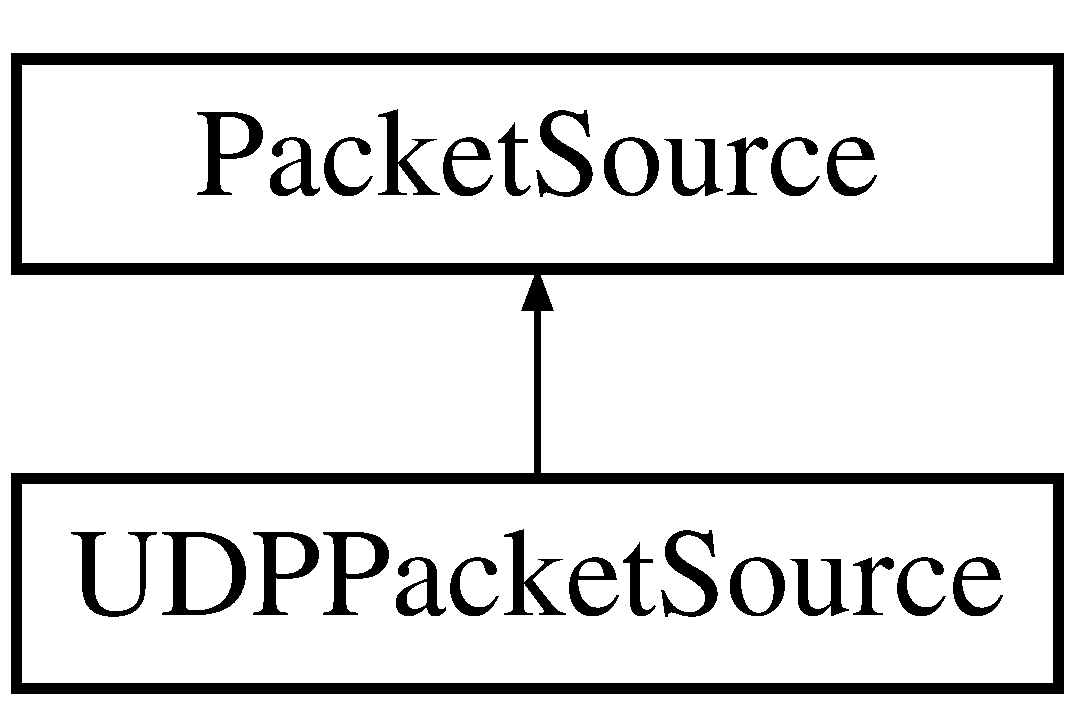
\includegraphics[height=2cm]{classPacketSource}
\end{center}
\end{figure}
\subsection*{Public Member Functions}
\begin{CompactItemize}
\item 
virtual {\bf $\sim$Packet\-Source} ()
\item 
virtual {\bf u\_\-int32\_\-t} {\bf recv} ({\bf Buffer} \&buf, std::string \&addr, {\bf u\_\-int16\_\-t} \&port)=0
\item 
virtual void {\bf send} ({\bf Buffer} \&buf, std::string addr, {\bf u\_\-int16\_\-t} port)=0
\end{CompactItemize}


\subsection{Constructor \& Destructor Documentation}
\index{PacketSource@{Packet\-Source}!~PacketSource@{$\sim$PacketSource}}
\index{~PacketSource@{$\sim$PacketSource}!PacketSource@{Packet\-Source}}
\subsubsection{\setlength{\rightskip}{0pt plus 5cm}virtual Packet\-Source::$\sim$Packet\-Source ()\hspace{0.3cm}{\tt  [inline, virtual]}}\label{classPacketSource_fdaad665e453cf5a047935b07a050ef4}




\subsection{Member Function Documentation}
\index{PacketSource@{Packet\-Source}!recv@{recv}}
\index{recv@{recv}!PacketSource@{Packet\-Source}}
\subsubsection{\setlength{\rightskip}{0pt plus 5cm}virtual {\bf u\_\-int32\_\-t} Packet\-Source::recv ({\bf Buffer} \& {\em buf}, std::string \& {\em addr}, {\bf u\_\-int16\_\-t} \& {\em port})\hspace{0.3cm}{\tt  [pure virtual]}}\label{classPacketSource_95901be715656540a7273c6c0dc1234e}




Implemented in {\bf UDPPacket\-Source} \doxyref{}{p.}{classUDPPacketSource_a1f7daded0f9ead5599160bae9317eb8}.\index{PacketSource@{Packet\-Source}!send@{send}}
\index{send@{send}!PacketSource@{Packet\-Source}}
\subsubsection{\setlength{\rightskip}{0pt plus 5cm}virtual void Packet\-Source::send ({\bf Buffer} \& {\em buf}, std::string {\em addr}, {\bf u\_\-int16\_\-t} {\em port})\hspace{0.3cm}{\tt  [pure virtual]}}\label{classPacketSource_ffc5eb2c89d1395443432c3cc6b7898b}




Implemented in {\bf UDPPacket\-Source} \doxyref{}{p.}{classUDPPacketSource_376a3b0c861aeb7561e8a9f6866292b9}.

The documentation for this class was generated from the following file:\begin{CompactItemize}
\item 
{\bf packet\-Source.h}\end{CompactItemize}

\section{Param Struct Reference}
\label{structParam}\index{Param@{Param}}
\subsection*{Public Attributes}
\begin{CompactItemize}
\item 
{\bf Options} \& {\bf opt}
\item 
{\bf Tun\-Device} \& {\bf dev}
\item 
{\bf Key\-Derivation} \& {\bf kd}
\item 
{\bf Cypher} \& {\bf c}
\item 
{\bf Auth\-Algo} \& {\bf a}
\item 
{\bf Packet\-Source} \& {\bf src}
\item 
{\bf Seq\-Window} \& {\bf seq}
\end{CompactItemize}


\subsection{Member Data Documentation}
\index{Param@{Param}!opt@{opt}}
\index{opt@{opt}!Param@{Param}}
\subsubsection{\setlength{\rightskip}{0pt plus 5cm}{\bf Options}\& {\bf Param::opt}}\label{structParam_f690604eb7652c5f5407815c5022b46c}


\index{Param@{Param}!dev@{dev}}
\index{dev@{dev}!Param@{Param}}
\subsubsection{\setlength{\rightskip}{0pt plus 5cm}{\bf Tun\-Device}\& {\bf Param::dev}}\label{structParam_1fa9d0f89264543bbad03a9e4e0c5f44}


\index{Param@{Param}!kd@{kd}}
\index{kd@{kd}!Param@{Param}}
\subsubsection{\setlength{\rightskip}{0pt plus 5cm}{\bf Key\-Derivation}\& {\bf Param::kd}}\label{structParam_6cfe55741cae1cf1bdde27561f292d8a}


\index{Param@{Param}!c@{c}}
\index{c@{c}!Param@{Param}}
\subsubsection{\setlength{\rightskip}{0pt plus 5cm}{\bf Cypher}\& {\bf Param::c}}\label{structParam_4ef5a8757e2f89fcb1317a1969641149}


\index{Param@{Param}!a@{a}}
\index{a@{a}!Param@{Param}}
\subsubsection{\setlength{\rightskip}{0pt plus 5cm}{\bf Auth\-Algo}\& {\bf Param::a}}\label{structParam_22172435ee2e6beb10acf92b2d68e40c}


\index{Param@{Param}!src@{src}}
\index{src@{src}!Param@{Param}}
\subsubsection{\setlength{\rightskip}{0pt plus 5cm}{\bf Packet\-Source}\& {\bf Param::src}}\label{structParam_fa5715cd7dc0833ea8f9afcbd1db455c}


\index{Param@{Param}!seq@{seq}}
\index{seq@{seq}!Param@{Param}}
\subsubsection{\setlength{\rightskip}{0pt plus 5cm}{\bf Seq\-Window}\& {\bf Param::seq}}\label{structParam_dc6a71f9fa352d3ecb312e2e33354f4e}




The documentation for this struct was generated from the following file:\begin{CompactItemize}
\item 
{\bf anytun.cpp}\end{CompactItemize}

\include{classRouter}
\section{satp::SATP Class Reference}
\label{classsatp_1_1SATP}\index{satp::SATP@{satp::SATP}}
Inheritance diagram for satp::SATP::\begin{figure}[H]
\begin{center}
\leavevmode
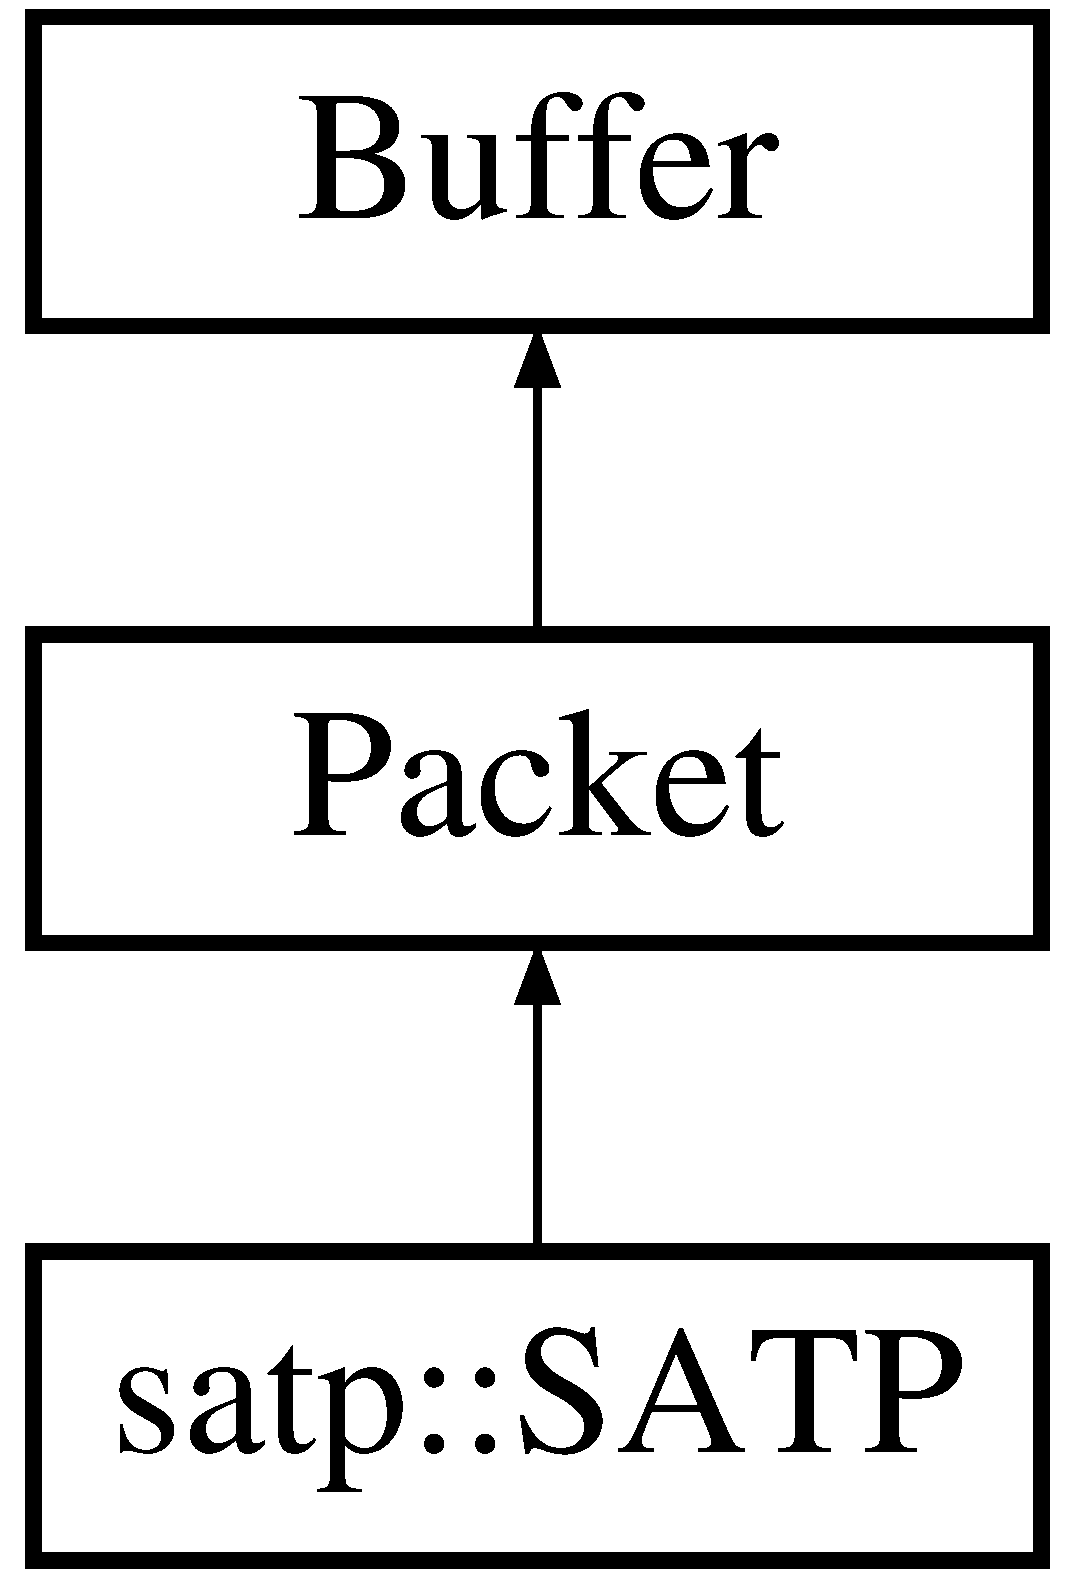
\includegraphics[height=3cm]{classsatp_1_1SATP}
\end{center}
\end{figure}
\subsection*{Static Public Attributes}
\begin{CompactItemize}
\item 
string {\bf name} = \char`\"{}SATP\char`\"{}
\item 
list {\bf fields\_\-desc}
\end{CompactItemize}


\subsection{Member Data Documentation}
\index{satp::SATP@{satp::SATP}!name@{name}}
\index{name@{name}!satp::SATP@{satp::SATP}}
\subsubsection{\setlength{\rightskip}{0pt plus 5cm}string {\bf satp::SATP::name} = \char`\"{}SATP\char`\"{}\hspace{0.3cm}{\tt  [static]}}\label{classsatp_1_1SATP_e9e415324a6a9fbe14971c1ffd334139}


\index{satp::SATP@{satp::SATP}!fields_desc@{fields\_\-desc}}
\index{fields_desc@{fields\_\-desc}!satp::SATP@{satp::SATP}}
\subsubsection{\setlength{\rightskip}{0pt plus 5cm}list {\bf satp::SATP::fields\_\-desc}\hspace{0.3cm}{\tt  [static]}}\label{classsatp_1_1SATP_e51015e8537b5ec7aa53ba87bf638c15}


\textbf{Initial value:}

\begin{Code}\begin{verbatim}[
            IntField("seq", None),
            ShortField("id", None)
            ]
\end{verbatim}\end{Code}


The documentation for this class was generated from the following file:\begin{CompactItemize}
\item 
{\bf satp.py}\end{CompactItemize}

\section{Semaphore Class Reference}
\label{classSemaphore}\index{Semaphore@{Semaphore}}
{\tt \#include $<$thread\-Utils.hpp$>$}

\subsection*{Public Member Functions}
\begin{CompactItemize}
\item 
{\bf Semaphore} (unsigned int init\-Val=0)
\item 
{\bf $\sim$Semaphore} ()
\item 
void {\bf down} ()
\item 
void {\bf up} ()
\end{CompactItemize}
\subsection*{Private Attributes}
\begin{CompactItemize}
\item 
sem\_\-t {\bf sem}
\end{CompactItemize}


\subsection{Constructor \& Destructor Documentation}
\index{Semaphore@{Semaphore}!Semaphore@{Semaphore}}
\index{Semaphore@{Semaphore}!Semaphore@{Semaphore}}
\subsubsection{\setlength{\rightskip}{0pt plus 5cm}Semaphore::Semaphore (unsigned int {\em init\-Val} = {\tt 0})\hspace{0.3cm}{\tt  [inline]}}\label{classSemaphore_570698c680a467b9b0a708635149d54a}


\index{Semaphore@{Semaphore}!~Semaphore@{$\sim$Semaphore}}
\index{~Semaphore@{$\sim$Semaphore}!Semaphore@{Semaphore}}
\subsubsection{\setlength{\rightskip}{0pt plus 5cm}Semaphore::$\sim$Semaphore ()\hspace{0.3cm}{\tt  [inline]}}\label{classSemaphore_633658a6fde276bffc912028725c6ade}




\subsection{Member Function Documentation}
\index{Semaphore@{Semaphore}!down@{down}}
\index{down@{down}!Semaphore@{Semaphore}}
\subsubsection{\setlength{\rightskip}{0pt plus 5cm}void Semaphore::down ()\hspace{0.3cm}{\tt  [inline]}}\label{classSemaphore_71126a13a22f2722e22a2b69860a5371}


\index{Semaphore@{Semaphore}!up@{up}}
\index{up@{up}!Semaphore@{Semaphore}}
\subsubsection{\setlength{\rightskip}{0pt plus 5cm}void Semaphore::up ()\hspace{0.3cm}{\tt  [inline]}}\label{classSemaphore_15fb190263808234fc2562f39f523082}




\subsection{Member Data Documentation}
\index{Semaphore@{Semaphore}!sem@{sem}}
\index{sem@{sem}!Semaphore@{Semaphore}}
\subsubsection{\setlength{\rightskip}{0pt plus 5cm}sem\_\-t {\bf Semaphore::sem}\hspace{0.3cm}{\tt  [private]}}\label{classSemaphore_23e62b0971c229ddf106e3ff71d688d6}




The documentation for this class was generated from the following file:\begin{CompactItemize}
\item 
{\bf thread\-Utils.hpp}\end{CompactItemize}

\section{Seq\-Window Class Reference}
\label{classSeqWindow}\index{SeqWindow@{SeqWindow}}
{\tt \#include $<$seq\-Window.h$>$}

\subsection*{Public Types}
\begin{CompactItemize}
\item 
typedef std::deque$<$ {\bf seq\_\-nr\_\-t} $>$ {\bf Seq\-Deque}
\item 
typedef std::map$<$ {\bf sender\_\-id\_\-t}, {\bf Seq\-Deque} $>$ {\bf Sender\-Map}
\end{CompactItemize}
\subsection*{Public Member Functions}
\begin{CompactItemize}
\item 
{\bf Seq\-Window} ({\bf window\_\-size\_\-t} w)
\item 
{\bf $\sim$Seq\-Window} ()
\item 
Seq\-Deque::size\_\-type {\bf get\-Length} ({\bf sender\_\-id\_\-t} sender)
\item 
bool {\bf has\-Seq\-Nr} ({\bf sender\_\-id\_\-t} sender, {\bf seq\_\-nr\_\-t} seq)
\item 
void {\bf add\-Seq\-Nr} ({\bf sender\_\-id\_\-t} sender, {\bf seq\_\-nr\_\-t} seq)
\item 
void {\bf clear} ({\bf sender\_\-id\_\-t} sender)
\item 
void {\bf clear} ()
\end{CompactItemize}
\subsection*{Private Member Functions}
\begin{CompactItemize}
\item 
{\bf Seq\-Window} (const {\bf Seq\-Window} \&s)
\item 
void {\bf operator=} (const {\bf Seq\-Window} \&s)
\end{CompactItemize}
\subsection*{Private Attributes}
\begin{CompactItemize}
\item 
{\bf window\_\-size\_\-t} {\bf window\_\-size\_\-}
\item 
{\bf Mutex} {\bf mutex\_\-}
\item 
{\bf Sender\-Map} {\bf sender\_\-}
\end{CompactItemize}


\subsection{Member Typedef Documentation}
\index{SeqWindow@{Seq\-Window}!SeqDeque@{SeqDeque}}
\index{SeqDeque@{SeqDeque}!SeqWindow@{Seq\-Window}}
\subsubsection{\setlength{\rightskip}{0pt plus 5cm}typedef std::deque$<${\bf seq\_\-nr\_\-t}$>$ {\bf Seq\-Window::Seq\-Deque}}\label{classSeqWindow_cf2d07003c8ca868146cffb4dd1d5ca7}


\index{SeqWindow@{Seq\-Window}!SenderMap@{SenderMap}}
\index{SenderMap@{SenderMap}!SeqWindow@{Seq\-Window}}
\subsubsection{\setlength{\rightskip}{0pt plus 5cm}typedef std::map$<${\bf sender\_\-id\_\-t}, {\bf Seq\-Deque}$>$ {\bf Seq\-Window::Sender\-Map}}\label{classSeqWindow_127195f139c8d5d07ed93799c2d6821a}




\subsection{Constructor \& Destructor Documentation}
\index{SeqWindow@{Seq\-Window}!SeqWindow@{SeqWindow}}
\index{SeqWindow@{SeqWindow}!SeqWindow@{Seq\-Window}}
\subsubsection{\setlength{\rightskip}{0pt plus 5cm}Seq\-Window::Seq\-Window ({\bf window\_\-size\_\-t} {\em w})}\label{classSeqWindow_8d513ab9ef2984ea93dad7e4026185c8}


\index{SeqWindow@{Seq\-Window}!~SeqWindow@{$\sim$SeqWindow}}
\index{~SeqWindow@{$\sim$SeqWindow}!SeqWindow@{Seq\-Window}}
\subsubsection{\setlength{\rightskip}{0pt plus 5cm}Seq\-Window::$\sim$Seq\-Window ()}\label{classSeqWindow_d125bcc4751a746427f04dda7fd65a10}


\index{SeqWindow@{Seq\-Window}!SeqWindow@{SeqWindow}}
\index{SeqWindow@{SeqWindow}!SeqWindow@{Seq\-Window}}
\subsubsection{\setlength{\rightskip}{0pt plus 5cm}Seq\-Window::Seq\-Window (const {\bf Seq\-Window} \& {\em s})\hspace{0.3cm}{\tt  [private]}}\label{classSeqWindow_7a30b232f312d843b8d188cae01fef28}




\subsection{Member Function Documentation}
\index{SeqWindow@{Seq\-Window}!getLength@{getLength}}
\index{getLength@{getLength}!SeqWindow@{Seq\-Window}}
\subsubsection{\setlength{\rightskip}{0pt plus 5cm}Seq\-Window::Seq\-Deque::size\_\-type Seq\-Window::get\-Length ({\bf sender\_\-id\_\-t} {\em sender})}\label{classSeqWindow_5d39959927c79c54d133ed77b297ad7c}


\index{SeqWindow@{Seq\-Window}!hasSeqNr@{hasSeqNr}}
\index{hasSeqNr@{hasSeqNr}!SeqWindow@{Seq\-Window}}
\subsubsection{\setlength{\rightskip}{0pt plus 5cm}bool Seq\-Window::has\-Seq\-Nr ({\bf sender\_\-id\_\-t} {\em sender}, {\bf seq\_\-nr\_\-t} {\em seq})}\label{classSeqWindow_9e7714dda181863420c38975bd505aff}


\index{SeqWindow@{Seq\-Window}!addSeqNr@{addSeqNr}}
\index{addSeqNr@{addSeqNr}!SeqWindow@{Seq\-Window}}
\subsubsection{\setlength{\rightskip}{0pt plus 5cm}void Seq\-Window::add\-Seq\-Nr ({\bf sender\_\-id\_\-t} {\em sender}, {\bf seq\_\-nr\_\-t} {\em seq})}\label{classSeqWindow_255ca0fca3e701bd9e18d9fcb2c022a2}


\index{SeqWindow@{Seq\-Window}!clear@{clear}}
\index{clear@{clear}!SeqWindow@{Seq\-Window}}
\subsubsection{\setlength{\rightskip}{0pt plus 5cm}void Seq\-Window::clear ({\bf sender\_\-id\_\-t} {\em sender})}\label{classSeqWindow_e9774163b8f7ac0ec081d1ba5b2daed2}


\index{SeqWindow@{Seq\-Window}!clear@{clear}}
\index{clear@{clear}!SeqWindow@{Seq\-Window}}
\subsubsection{\setlength{\rightskip}{0pt plus 5cm}void Seq\-Window::clear ()}\label{classSeqWindow_b1a03fe152c7c94ff3f05005d595b424}


\index{SeqWindow@{Seq\-Window}!operator=@{operator=}}
\index{operator=@{operator=}!SeqWindow@{Seq\-Window}}
\subsubsection{\setlength{\rightskip}{0pt plus 5cm}void Seq\-Window::operator= (const {\bf Seq\-Window} \& {\em s})\hspace{0.3cm}{\tt  [private]}}\label{classSeqWindow_37887e66297163fe301c77f2977a2a2b}




\subsection{Member Data Documentation}
\index{SeqWindow@{Seq\-Window}!window_size_@{window\_\-size\_\-}}
\index{window_size_@{window\_\-size\_\-}!SeqWindow@{Seq\-Window}}
\subsubsection{\setlength{\rightskip}{0pt plus 5cm}{\bf window\_\-size\_\-t} {\bf Seq\-Window::window\_\-size\_\-}\hspace{0.3cm}{\tt  [private]}}\label{classSeqWindow_ef85ba28f8a655dc8c8d34aeddb8eea0}


\index{SeqWindow@{Seq\-Window}!mutex_@{mutex\_\-}}
\index{mutex_@{mutex\_\-}!SeqWindow@{Seq\-Window}}
\subsubsection{\setlength{\rightskip}{0pt plus 5cm}{\bf Mutex} {\bf Seq\-Window::mutex\_\-}\hspace{0.3cm}{\tt  [private]}}\label{classSeqWindow_87ec44a9a7398ecbcb92d90ba95b37a0}


\index{SeqWindow@{Seq\-Window}!sender_@{sender\_\-}}
\index{sender_@{sender\_\-}!SeqWindow@{Seq\-Window}}
\subsubsection{\setlength{\rightskip}{0pt plus 5cm}{\bf Sender\-Map} {\bf Seq\-Window::sender\_\-}\hspace{0.3cm}{\tt  [private]}}\label{classSeqWindow_8bfc3742cacc75e9a72de13ff6ad98a2}




The documentation for this class was generated from the following files:\begin{CompactItemize}
\item 
{\bf seq\-Window.h}\item 
{\bf seq\-Window.cpp}\end{CompactItemize}

\section{Sig\-Hup\-Handler Class Reference}
\label{classSigHupHandler}\index{SigHupHandler@{SigHupHandler}}
{\tt \#include $<$signal\-Controller.h$>$}

Inheritance diagram for Sig\-Hup\-Handler::\begin{figure}[H]
\begin{center}
\leavevmode
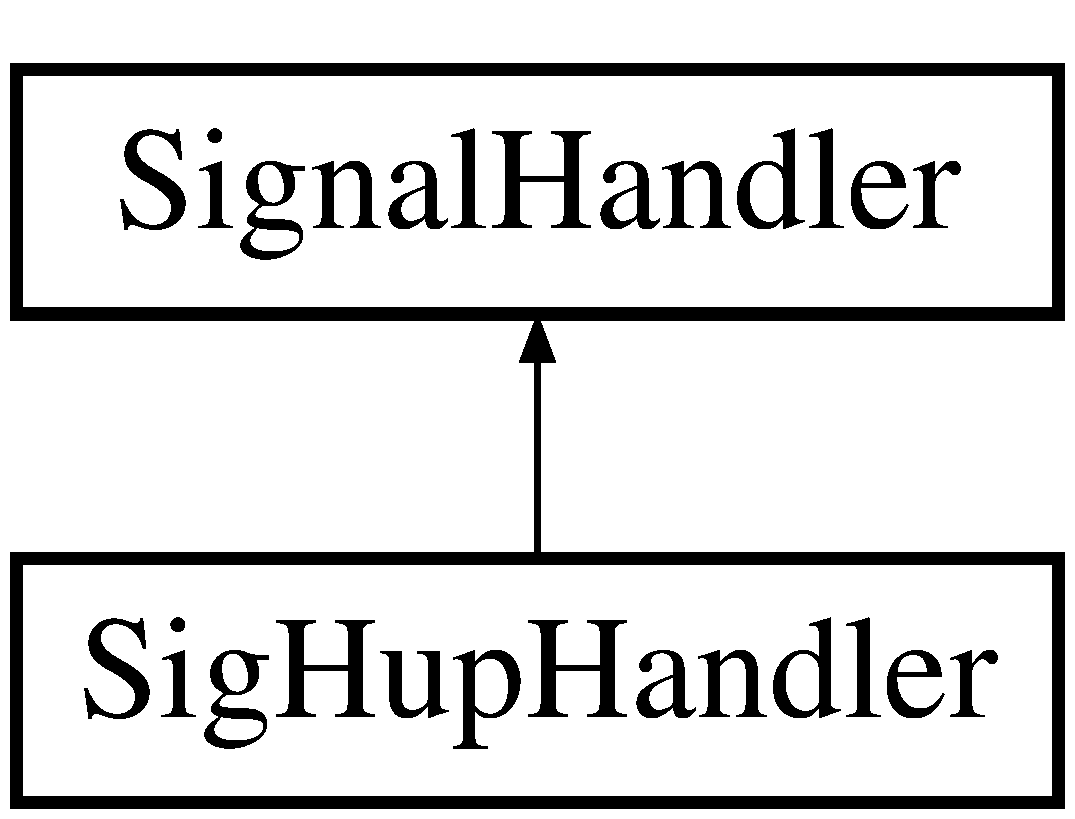
\includegraphics[height=2cm]{classSigHupHandler}
\end{center}
\end{figure}
\subsection*{Public Member Functions}
\begin{CompactItemize}
\item 
{\bf Sig\-Hup\-Handler} ()
\item 
int {\bf handle} ()
\end{CompactItemize}


\subsection{Constructor \& Destructor Documentation}
\index{SigHupHandler@{Sig\-Hup\-Handler}!SigHupHandler@{SigHupHandler}}
\index{SigHupHandler@{SigHupHandler}!SigHupHandler@{Sig\-Hup\-Handler}}
\subsubsection{\setlength{\rightskip}{0pt plus 5cm}Sig\-Hup\-Handler::Sig\-Hup\-Handler ()\hspace{0.3cm}{\tt  [inline]}}\label{classSigHupHandler_a1ee03b63ca11d8b5aae82fae1f2d6a3}




\subsection{Member Function Documentation}
\index{SigHupHandler@{Sig\-Hup\-Handler}!handle@{handle}}
\index{handle@{handle}!SigHupHandler@{Sig\-Hup\-Handler}}
\subsubsection{\setlength{\rightskip}{0pt plus 5cm}int Sig\-Hup\-Handler::handle ()\hspace{0.3cm}{\tt  [virtual]}}\label{classSigHupHandler_84734b7f79663badeedb720896302d4e}




Reimplemented from {\bf Signal\-Handler} \doxyref{}{p.}{classSignalHandler_e3dbda0de9b4aa4544390818a0d29e28}.

The documentation for this class was generated from the following files:\begin{CompactItemize}
\item 
{\bf signal\-Controller.h}\item 
{\bf signal\-Controller.cpp}\end{CompactItemize}

\section{Sig\-Int\-Handler Class Reference}
\label{classSigIntHandler}\index{SigIntHandler@{SigIntHandler}}
{\tt \#include $<$signal\-Controller.h$>$}

Inheritance diagram for Sig\-Int\-Handler::\begin{figure}[H]
\begin{center}
\leavevmode
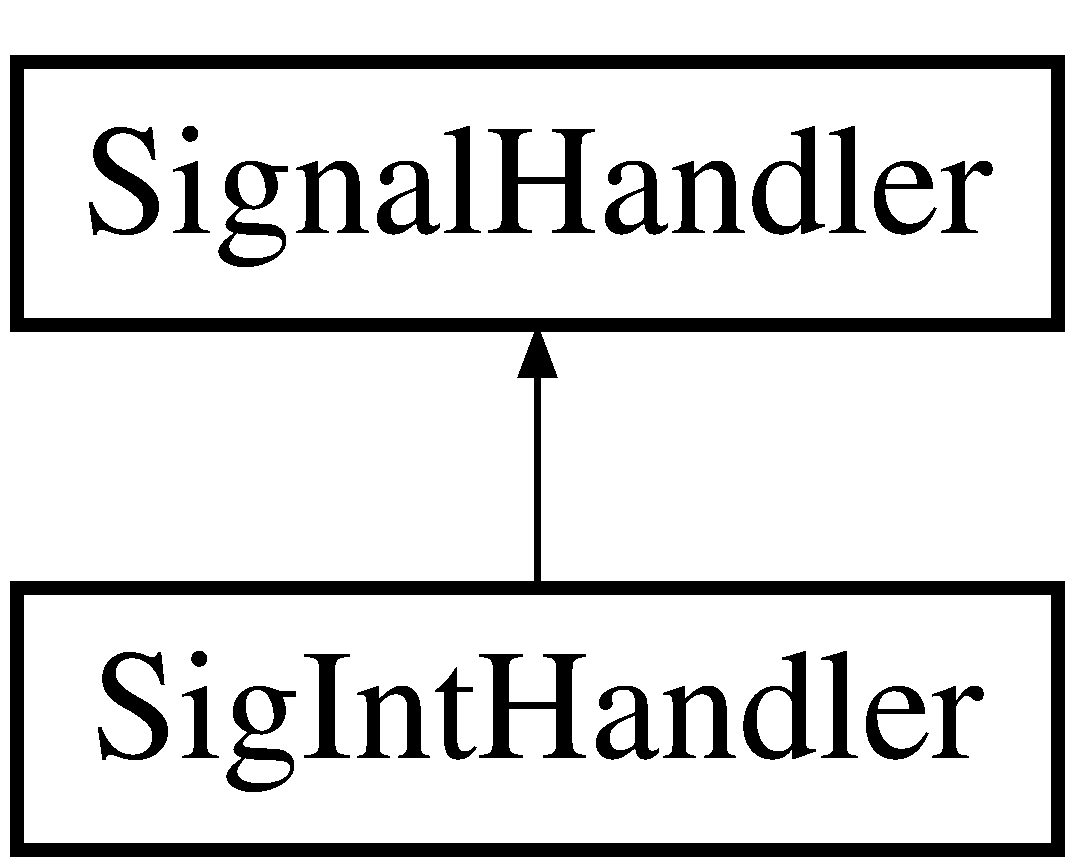
\includegraphics[height=2cm]{classSigIntHandler}
\end{center}
\end{figure}
\subsection*{Public Member Functions}
\begin{CompactItemize}
\item 
{\bf Sig\-Int\-Handler} ()
\item 
int {\bf handle} ()
\end{CompactItemize}


\subsection{Constructor \& Destructor Documentation}
\index{SigIntHandler@{Sig\-Int\-Handler}!SigIntHandler@{SigIntHandler}}
\index{SigIntHandler@{SigIntHandler}!SigIntHandler@{Sig\-Int\-Handler}}
\subsubsection{\setlength{\rightskip}{0pt plus 5cm}Sig\-Int\-Handler::Sig\-Int\-Handler ()\hspace{0.3cm}{\tt  [inline]}}\label{classSigIntHandler_ac25b5ac048a76d4c0c26d5ad4c4273d}




\subsection{Member Function Documentation}
\index{SigIntHandler@{Sig\-Int\-Handler}!handle@{handle}}
\index{handle@{handle}!SigIntHandler@{Sig\-Int\-Handler}}
\subsubsection{\setlength{\rightskip}{0pt plus 5cm}int Sig\-Int\-Handler::handle ()\hspace{0.3cm}{\tt  [virtual]}}\label{classSigIntHandler_6a7d9a841a5c9b1f50041a8c37774063}




Reimplemented from {\bf Signal\-Handler} \doxyref{}{p.}{classSignalHandler_e3dbda0de9b4aa4544390818a0d29e28}.

The documentation for this class was generated from the following files:\begin{CompactItemize}
\item 
{\bf signal\-Controller.h}\item 
{\bf signal\-Controller.cpp}\end{CompactItemize}

\section{Signal\-Controller Class Reference}
\label{classSignalController}\index{SignalController@{SignalController}}
{\tt \#include $<$signal\-Controller.h$>$}

\subsection*{Public Member Functions}
\begin{CompactItemize}
\item 
{\bf Signal\-Controller} ()
\item 
{\bf $\sim$Signal\-Controller} ()
\item 
void {\bf init} ()
\item 
int {\bf run} ()
\end{CompactItemize}
\subsection*{Static Public Member Functions}
\begin{CompactItemize}
\item 
static void $\ast$ {\bf handle} (void $\ast$s)
\end{CompactItemize}
\subsection*{Private Types}
\begin{CompactItemize}
\item 
typedef std::map$<$ int, {\bf Signal\-Handler} $\ast$ $>$ {\bf Handler\-Map}
\end{CompactItemize}
\subsection*{Private Member Functions}
\begin{CompactItemize}
\item 
{\bf Signal\-Controller} (const {\bf Signal\-Controller} \&s)
\item 
void {\bf operator=} (const {\bf Signal\-Controller} \&s)
\end{CompactItemize}
\subsection*{Private Attributes}
\begin{CompactItemize}
\item 
std::queue$<$ int $>$ {\bf sig\-Queue}
\item 
{\bf Mutex} {\bf sig\-Queue\-Mutex}
\item 
{\bf Semaphore} {\bf sig\-Queue\-Sem}
\item 
pthread\_\-t {\bf thread}
\item 
{\bf Handler\-Map} {\bf handler}
\end{CompactItemize}


\subsection{Member Typedef Documentation}
\index{SignalController@{Signal\-Controller}!HandlerMap@{HandlerMap}}
\index{HandlerMap@{HandlerMap}!SignalController@{Signal\-Controller}}
\subsubsection{\setlength{\rightskip}{0pt plus 5cm}typedef std::map$<$int, {\bf Signal\-Handler}$\ast$$>$ {\bf Signal\-Controller::Handler\-Map}\hspace{0.3cm}{\tt  [private]}}\label{classSignalController_659eb661ef3d40565d739a50bbe4b554}




\subsection{Constructor \& Destructor Documentation}
\index{SignalController@{Signal\-Controller}!SignalController@{SignalController}}
\index{SignalController@{SignalController}!SignalController@{Signal\-Controller}}
\subsubsection{\setlength{\rightskip}{0pt plus 5cm}Signal\-Controller::Signal\-Controller ()\hspace{0.3cm}{\tt  [inline]}}\label{classSignalController_d057c96011d444cce15e2a398a0a8bbf}


\index{SignalController@{Signal\-Controller}!~SignalController@{$\sim$SignalController}}
\index{~SignalController@{$\sim$SignalController}!SignalController@{Signal\-Controller}}
\subsubsection{\setlength{\rightskip}{0pt plus 5cm}Signal\-Controller::$\sim$Signal\-Controller ()}\label{classSignalController_e8d687dc4fcc75bffff50e8cda37c7aa}


\index{SignalController@{Signal\-Controller}!SignalController@{SignalController}}
\index{SignalController@{SignalController}!SignalController@{Signal\-Controller}}
\subsubsection{\setlength{\rightskip}{0pt plus 5cm}Signal\-Controller::Signal\-Controller (const {\bf Signal\-Controller} \& {\em s})\hspace{0.3cm}{\tt  [private]}}\label{classSignalController_31af143ea1219cd000abe91aeccc84bc}




\subsection{Member Function Documentation}
\index{SignalController@{Signal\-Controller}!handle@{handle}}
\index{handle@{handle}!SignalController@{Signal\-Controller}}
\subsubsection{\setlength{\rightskip}{0pt plus 5cm}void $\ast$ Signal\-Controller::handle (void $\ast$ {\em s})\hspace{0.3cm}{\tt  [static]}}\label{classSignalController_5df4d6ebe373117a9bf072035e16997f}


\index{SignalController@{Signal\-Controller}!init@{init}}
\index{init@{init}!SignalController@{Signal\-Controller}}
\subsubsection{\setlength{\rightskip}{0pt plus 5cm}void Signal\-Controller::init ()}\label{classSignalController_0d66065172b1c7ac0d55757d178e6911}


\index{SignalController@{Signal\-Controller}!run@{run}}
\index{run@{run}!SignalController@{Signal\-Controller}}
\subsubsection{\setlength{\rightskip}{0pt plus 5cm}int Signal\-Controller::run ()}\label{classSignalController_0f7657b70cb2e8457539d9f844a93619}


\index{SignalController@{Signal\-Controller}!operator=@{operator=}}
\index{operator=@{operator=}!SignalController@{Signal\-Controller}}
\subsubsection{\setlength{\rightskip}{0pt plus 5cm}void Signal\-Controller::operator= (const {\bf Signal\-Controller} \& {\em s})\hspace{0.3cm}{\tt  [private]}}\label{classSignalController_7bfe78f3e8c5d40ddd51c313d30cf6a2}




\subsection{Member Data Documentation}
\index{SignalController@{Signal\-Controller}!sigQueue@{sigQueue}}
\index{sigQueue@{sigQueue}!SignalController@{Signal\-Controller}}
\subsubsection{\setlength{\rightskip}{0pt plus 5cm}std::queue$<$int$>$ {\bf Signal\-Controller::sig\-Queue}\hspace{0.3cm}{\tt  [private]}}\label{classSignalController_543fa6d49a071df92cdfcc7bc96de161}


\index{SignalController@{Signal\-Controller}!sigQueueMutex@{sigQueueMutex}}
\index{sigQueueMutex@{sigQueueMutex}!SignalController@{Signal\-Controller}}
\subsubsection{\setlength{\rightskip}{0pt plus 5cm}{\bf Mutex} {\bf Signal\-Controller::sig\-Queue\-Mutex}\hspace{0.3cm}{\tt  [private]}}\label{classSignalController_6b7853059aa422fac6c2cc77e00d28ee}


\index{SignalController@{Signal\-Controller}!sigQueueSem@{sigQueueSem}}
\index{sigQueueSem@{sigQueueSem}!SignalController@{Signal\-Controller}}
\subsubsection{\setlength{\rightskip}{0pt plus 5cm}{\bf Semaphore} {\bf Signal\-Controller::sig\-Queue\-Sem}\hspace{0.3cm}{\tt  [private]}}\label{classSignalController_4dfee82061341e1af5ca827333c8bd10}


\index{SignalController@{Signal\-Controller}!thread@{thread}}
\index{thread@{thread}!SignalController@{Signal\-Controller}}
\subsubsection{\setlength{\rightskip}{0pt plus 5cm}pthread\_\-t {\bf Signal\-Controller::thread}\hspace{0.3cm}{\tt  [private]}}\label{classSignalController_79c5fbfa55aa9edc2a45c5ed3197b782}


\index{SignalController@{Signal\-Controller}!handler@{handler}}
\index{handler@{handler}!SignalController@{Signal\-Controller}}
\subsubsection{\setlength{\rightskip}{0pt plus 5cm}{\bf Handler\-Map} {\bf Signal\-Controller::handler}\hspace{0.3cm}{\tt  [private]}}\label{classSignalController_f76d2f570d55019dd15921eba71efe0b}




The documentation for this class was generated from the following files:\begin{CompactItemize}
\item 
{\bf signal\-Controller.h}\item 
{\bf signal\-Controller.cpp}\end{CompactItemize}

\section{Signal\-Handler Class Reference}
\label{classSignalHandler}\index{SignalHandler@{SignalHandler}}
{\tt \#include $<$signal\-Controller.h$>$}

Inheritance diagram for Signal\-Handler::\begin{figure}[H]
\begin{center}
\leavevmode
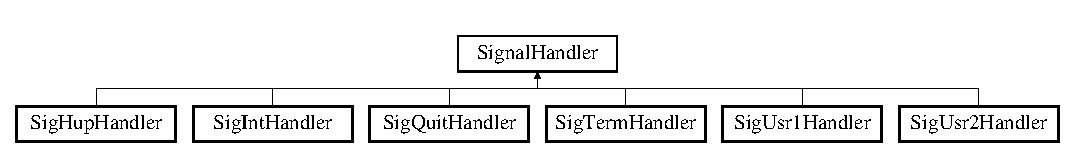
\includegraphics[height=1.68168cm]{classSignalHandler}
\end{center}
\end{figure}
\subsection*{Public Member Functions}
\begin{CompactItemize}
\item 
virtual {\bf $\sim$Signal\-Handler} ()
\item 
virtual int {\bf handle} ()
\end{CompactItemize}
\subsection*{Protected Member Functions}
\begin{CompactItemize}
\item 
{\bf Signal\-Handler} (int s)
\end{CompactItemize}
\subsection*{Private Attributes}
\begin{CompactItemize}
\item 
int {\bf sig\-Num}
\end{CompactItemize}
\subsection*{Friends}
\begin{CompactItemize}
\item 
class {\bf Signal\-Controller}
\end{CompactItemize}


\subsection{Constructor \& Destructor Documentation}
\index{SignalHandler@{Signal\-Handler}!~SignalHandler@{$\sim$SignalHandler}}
\index{~SignalHandler@{$\sim$SignalHandler}!SignalHandler@{Signal\-Handler}}
\subsubsection{\setlength{\rightskip}{0pt plus 5cm}virtual Signal\-Handler::$\sim$Signal\-Handler ()\hspace{0.3cm}{\tt  [inline, virtual]}}\label{classSignalHandler_a1109d38f8b43bde75420aaeecc1f2b7}


\index{SignalHandler@{Signal\-Handler}!SignalHandler@{SignalHandler}}
\index{SignalHandler@{SignalHandler}!SignalHandler@{Signal\-Handler}}
\subsubsection{\setlength{\rightskip}{0pt plus 5cm}Signal\-Handler::Signal\-Handler (int {\em s})\hspace{0.3cm}{\tt  [inline, protected]}}\label{classSignalHandler_8f920534650e9cd3cdfbe3c3f8409b4d}




\subsection{Member Function Documentation}
\index{SignalHandler@{Signal\-Handler}!handle@{handle}}
\index{handle@{handle}!SignalHandler@{Signal\-Handler}}
\subsubsection{\setlength{\rightskip}{0pt plus 5cm}virtual int Signal\-Handler::handle ()\hspace{0.3cm}{\tt  [inline, virtual]}}\label{classSignalHandler_e3dbda0de9b4aa4544390818a0d29e28}




Reimplemented in {\bf Sig\-Int\-Handler} \doxyref{}{p.}{classSigIntHandler_6a7d9a841a5c9b1f50041a8c37774063}, {\bf Sig\-Quit\-Handler} \doxyref{}{p.}{classSigQuitHandler_799f0272c91e7b1bf09411b80811b4dc}, {\bf Sig\-Hup\-Handler} \doxyref{}{p.}{classSigHupHandler_84734b7f79663badeedb720896302d4e}, {\bf Sig\-Usr1Handler} \doxyref{}{p.}{classSigUsr1Handler_578f3ea18e617689032fc165b6436695}, {\bf Sig\-Usr2Handler} \doxyref{}{p.}{classSigUsr2Handler_825a621f1ff10556bb8b289703273e7d}, and {\bf Sig\-Term\-Handler} \doxyref{}{p.}{classSigTermHandler_820fa7f8bb5ef6390133c33c919dbf6f}.

\subsection{Friends And Related Function Documentation}
\index{SignalHandler@{Signal\-Handler}!SignalController@{SignalController}}
\index{SignalController@{SignalController}!SignalHandler@{Signal\-Handler}}
\subsubsection{\setlength{\rightskip}{0pt plus 5cm}friend class {\bf Signal\-Controller}\hspace{0.3cm}{\tt  [friend]}}\label{classSignalHandler_9b5c65d0274d45f20c9ed28852dd66fa}




\subsection{Member Data Documentation}
\index{SignalHandler@{Signal\-Handler}!sigNum@{sigNum}}
\index{sigNum@{sigNum}!SignalHandler@{Signal\-Handler}}
\subsubsection{\setlength{\rightskip}{0pt plus 5cm}int {\bf Signal\-Handler::sig\-Num}\hspace{0.3cm}{\tt  [private]}}\label{classSignalHandler_0585573af0ea6bebf37bda54e5c3c39d}




The documentation for this class was generated from the following file:\begin{CompactItemize}
\item 
{\bf signal\-Controller.h}\end{CompactItemize}

\section{Sig\-Quit\-Handler Class Reference}
\label{classSigQuitHandler}\index{SigQuitHandler@{SigQuitHandler}}
{\tt \#include $<$signal\-Controller.h$>$}

Inheritance diagram for Sig\-Quit\-Handler::\begin{figure}[H]
\begin{center}
\leavevmode
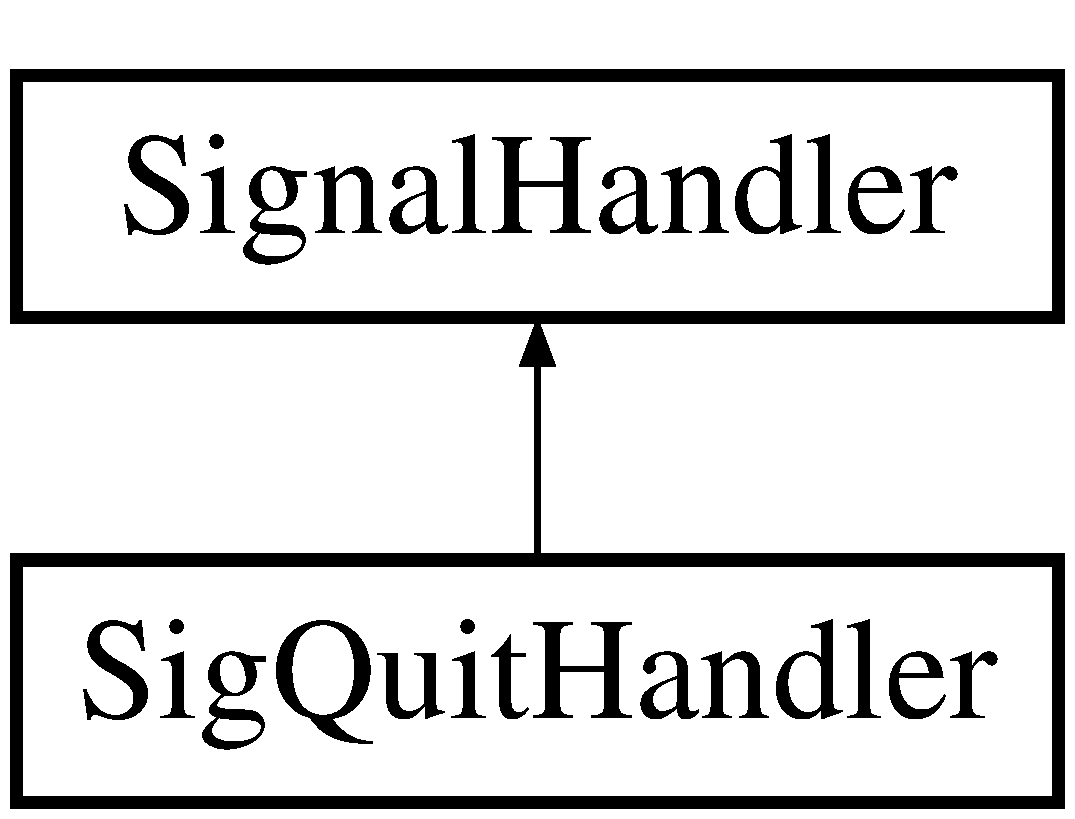
\includegraphics[height=2cm]{classSigQuitHandler}
\end{center}
\end{figure}
\subsection*{Public Member Functions}
\begin{CompactItemize}
\item 
{\bf Sig\-Quit\-Handler} ()
\item 
int {\bf handle} ()
\end{CompactItemize}


\subsection{Constructor \& Destructor Documentation}
\index{SigQuitHandler@{Sig\-Quit\-Handler}!SigQuitHandler@{SigQuitHandler}}
\index{SigQuitHandler@{SigQuitHandler}!SigQuitHandler@{Sig\-Quit\-Handler}}
\subsubsection{\setlength{\rightskip}{0pt plus 5cm}Sig\-Quit\-Handler::Sig\-Quit\-Handler ()\hspace{0.3cm}{\tt  [inline]}}\label{classSigQuitHandler_45885e5ddfa14f9bfc13c72de425e1c6}




\subsection{Member Function Documentation}
\index{SigQuitHandler@{Sig\-Quit\-Handler}!handle@{handle}}
\index{handle@{handle}!SigQuitHandler@{Sig\-Quit\-Handler}}
\subsubsection{\setlength{\rightskip}{0pt plus 5cm}int Sig\-Quit\-Handler::handle ()\hspace{0.3cm}{\tt  [virtual]}}\label{classSigQuitHandler_799f0272c91e7b1bf09411b80811b4dc}




Reimplemented from {\bf Signal\-Handler} \doxyref{}{p.}{classSignalHandler_e3dbda0de9b4aa4544390818a0d29e28}.

The documentation for this class was generated from the following files:\begin{CompactItemize}
\item 
{\bf signal\-Controller.h}\item 
{\bf signal\-Controller.cpp}\end{CompactItemize}

\section{Sig\-Term\-Handler Class Reference}
\label{classSigTermHandler}\index{SigTermHandler@{SigTermHandler}}
{\tt \#include $<$signal\-Controller.h$>$}

Inheritance diagram for Sig\-Term\-Handler::\begin{figure}[H]
\begin{center}
\leavevmode
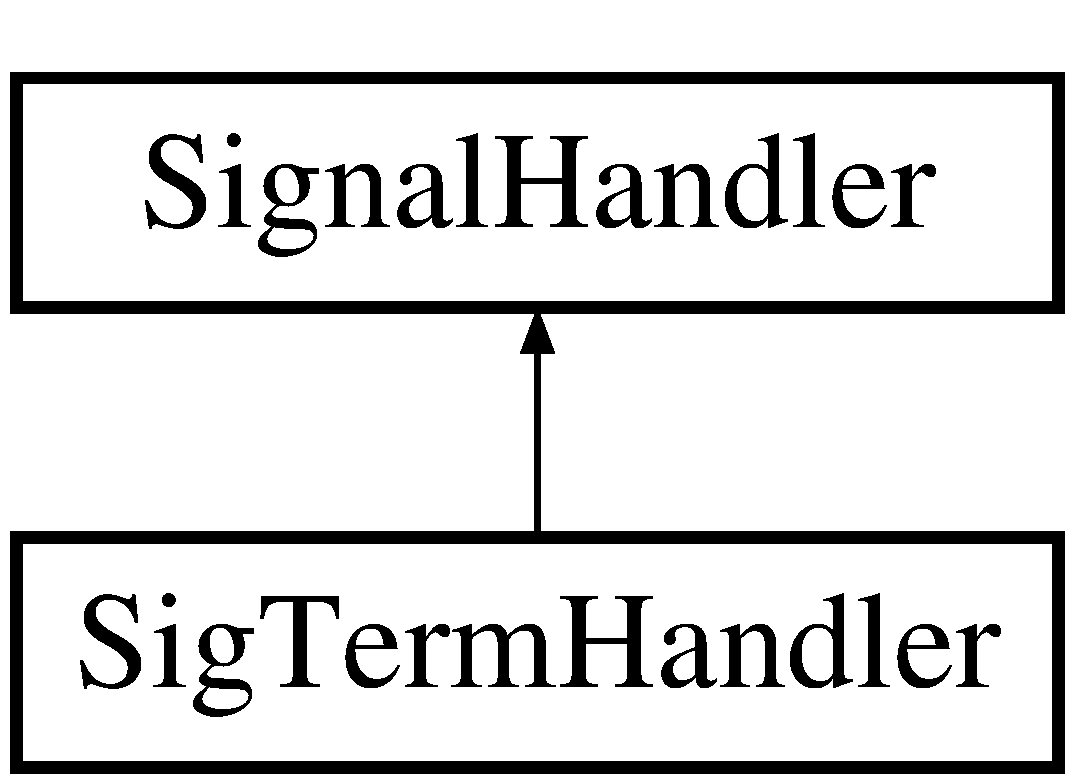
\includegraphics[height=2cm]{classSigTermHandler}
\end{center}
\end{figure}
\subsection*{Public Member Functions}
\begin{CompactItemize}
\item 
{\bf Sig\-Term\-Handler} ()
\item 
int {\bf handle} ()
\end{CompactItemize}


\subsection{Constructor \& Destructor Documentation}
\index{SigTermHandler@{Sig\-Term\-Handler}!SigTermHandler@{SigTermHandler}}
\index{SigTermHandler@{SigTermHandler}!SigTermHandler@{Sig\-Term\-Handler}}
\subsubsection{\setlength{\rightskip}{0pt plus 5cm}Sig\-Term\-Handler::Sig\-Term\-Handler ()\hspace{0.3cm}{\tt  [inline]}}\label{classSigTermHandler_8f6c3da13e1ec7fc8ef122bd0db457e4}




\subsection{Member Function Documentation}
\index{SigTermHandler@{Sig\-Term\-Handler}!handle@{handle}}
\index{handle@{handle}!SigTermHandler@{Sig\-Term\-Handler}}
\subsubsection{\setlength{\rightskip}{0pt plus 5cm}int Sig\-Term\-Handler::handle ()\hspace{0.3cm}{\tt  [virtual]}}\label{classSigTermHandler_820fa7f8bb5ef6390133c33c919dbf6f}




Reimplemented from {\bf Signal\-Handler} \doxyref{}{p.}{classSignalHandler_e3dbda0de9b4aa4544390818a0d29e28}.

The documentation for this class was generated from the following files:\begin{CompactItemize}
\item 
{\bf signal\-Controller.h}\item 
{\bf signal\-Controller.cpp}\end{CompactItemize}

\section{Sig\-Usr1Handler Class Reference}
\label{classSigUsr1Handler}\index{SigUsr1Handler@{SigUsr1Handler}}
{\tt \#include $<$signal\-Controller.h$>$}

Inheritance diagram for Sig\-Usr1Handler::\begin{figure}[H]
\begin{center}
\leavevmode
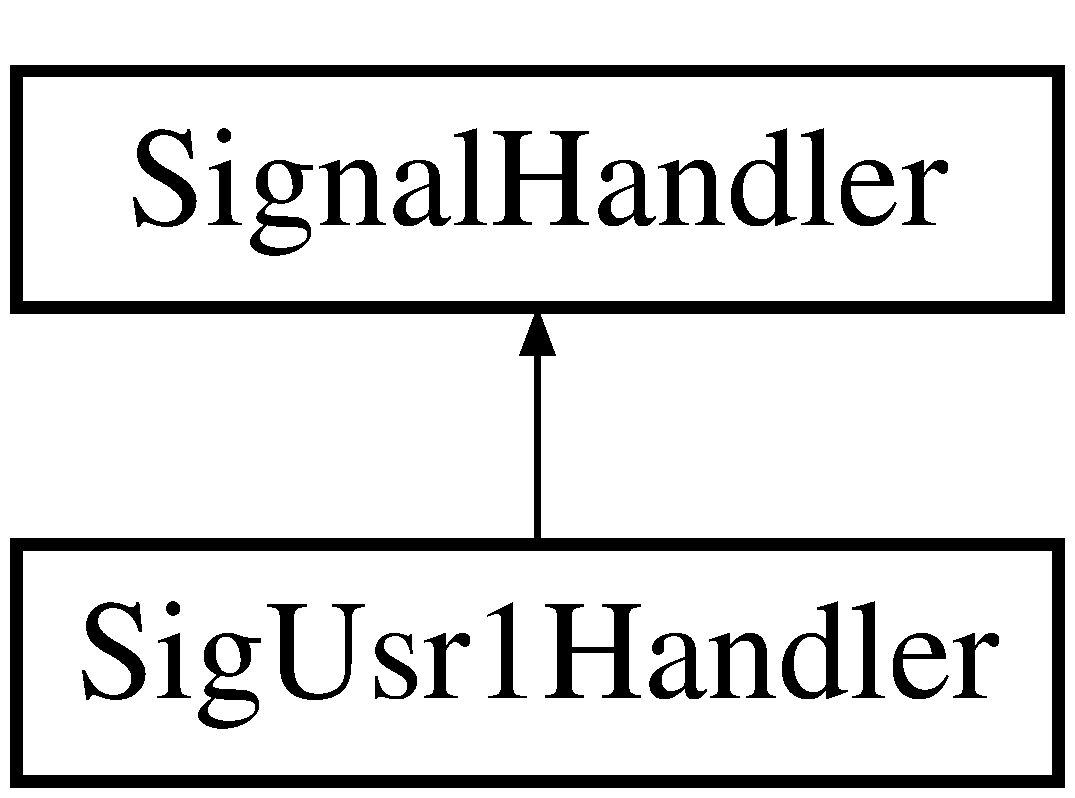
\includegraphics[height=2cm]{classSigUsr1Handler}
\end{center}
\end{figure}
\subsection*{Public Member Functions}
\begin{CompactItemize}
\item 
{\bf Sig\-Usr1Handler} ()
\item 
int {\bf handle} ()
\end{CompactItemize}


\subsection{Constructor \& Destructor Documentation}
\index{SigUsr1Handler@{Sig\-Usr1Handler}!SigUsr1Handler@{SigUsr1Handler}}
\index{SigUsr1Handler@{SigUsr1Handler}!SigUsr1Handler@{Sig\-Usr1Handler}}
\subsubsection{\setlength{\rightskip}{0pt plus 5cm}Sig\-Usr1Handler::Sig\-Usr1Handler ()\hspace{0.3cm}{\tt  [inline]}}\label{classSigUsr1Handler_aabaa57b0f2bb331a85f95cf90dd121d}




\subsection{Member Function Documentation}
\index{SigUsr1Handler@{Sig\-Usr1Handler}!handle@{handle}}
\index{handle@{handle}!SigUsr1Handler@{Sig\-Usr1Handler}}
\subsubsection{\setlength{\rightskip}{0pt plus 5cm}int Sig\-Usr1Handler::handle ()\hspace{0.3cm}{\tt  [virtual]}}\label{classSigUsr1Handler_578f3ea18e617689032fc165b6436695}




Reimplemented from {\bf Signal\-Handler} \doxyref{}{p.}{classSignalHandler_e3dbda0de9b4aa4544390818a0d29e28}.

The documentation for this class was generated from the following files:\begin{CompactItemize}
\item 
{\bf signal\-Controller.h}\item 
{\bf signal\-Controller.cpp}\end{CompactItemize}

\section{Sig\-Usr2Handler Class Reference}
\label{classSigUsr2Handler}\index{SigUsr2Handler@{SigUsr2Handler}}
{\tt \#include $<$signal\-Controller.h$>$}

Inheritance diagram for Sig\-Usr2Handler::\begin{figure}[H]
\begin{center}
\leavevmode
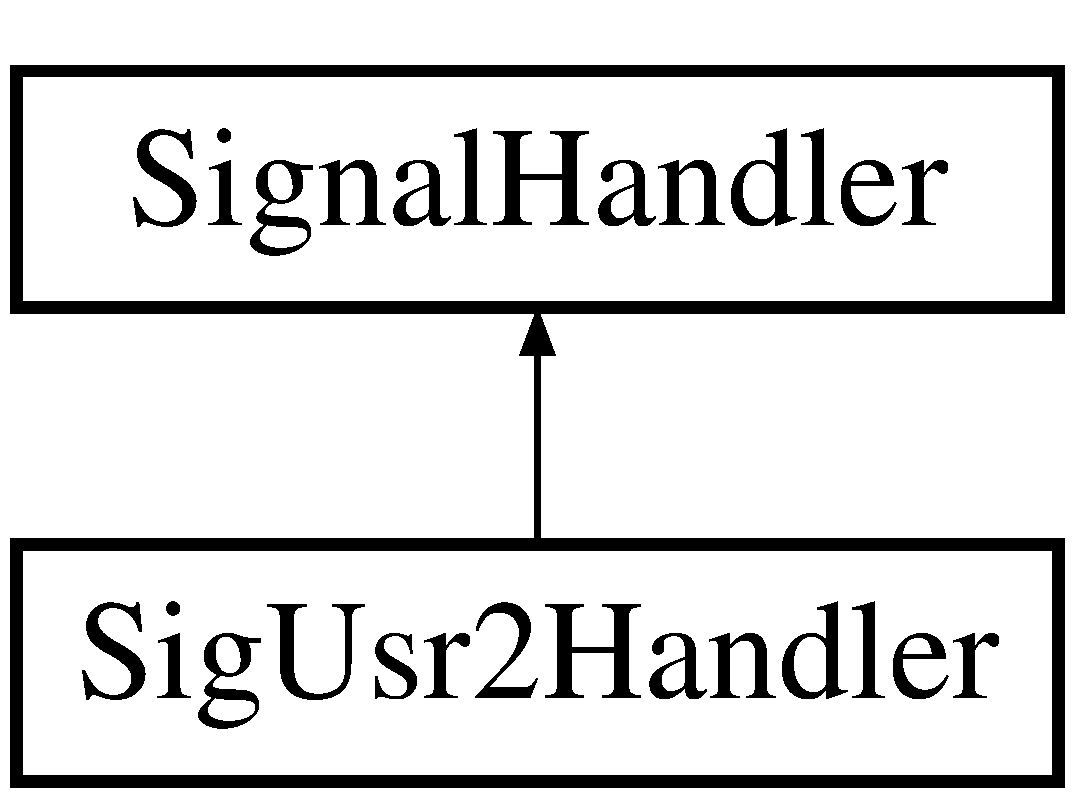
\includegraphics[height=2cm]{classSigUsr2Handler}
\end{center}
\end{figure}
\subsection*{Public Member Functions}
\begin{CompactItemize}
\item 
{\bf Sig\-Usr2Handler} ()
\item 
int {\bf handle} ()
\end{CompactItemize}


\subsection{Constructor \& Destructor Documentation}
\index{SigUsr2Handler@{Sig\-Usr2Handler}!SigUsr2Handler@{SigUsr2Handler}}
\index{SigUsr2Handler@{SigUsr2Handler}!SigUsr2Handler@{Sig\-Usr2Handler}}
\subsubsection{\setlength{\rightskip}{0pt plus 5cm}Sig\-Usr2Handler::Sig\-Usr2Handler ()\hspace{0.3cm}{\tt  [inline]}}\label{classSigUsr2Handler_30478acdc28555b412d80f1419af622a}




\subsection{Member Function Documentation}
\index{SigUsr2Handler@{Sig\-Usr2Handler}!handle@{handle}}
\index{handle@{handle}!SigUsr2Handler@{Sig\-Usr2Handler}}
\subsubsection{\setlength{\rightskip}{0pt plus 5cm}int Sig\-Usr2Handler::handle ()\hspace{0.3cm}{\tt  [virtual]}}\label{classSigUsr2Handler_825a621f1ff10556bb8b289703273e7d}




Reimplemented from {\bf Signal\-Handler} \doxyref{}{p.}{classSignalHandler_e3dbda0de9b4aa4544390818a0d29e28}.

The documentation for this class was generated from the following files:\begin{CompactItemize}
\item 
{\bf signal\-Controller.h}\item 
{\bf signal\-Controller.cpp}\end{CompactItemize}

\section{Socket Class Reference}
\label{classSocket}\index{Socket@{Socket}}
{\tt \#include $<$Practical\-Socket.h$>$}

Inheritance diagram for Socket::\begin{figure}[H]
\begin{center}
\leavevmode
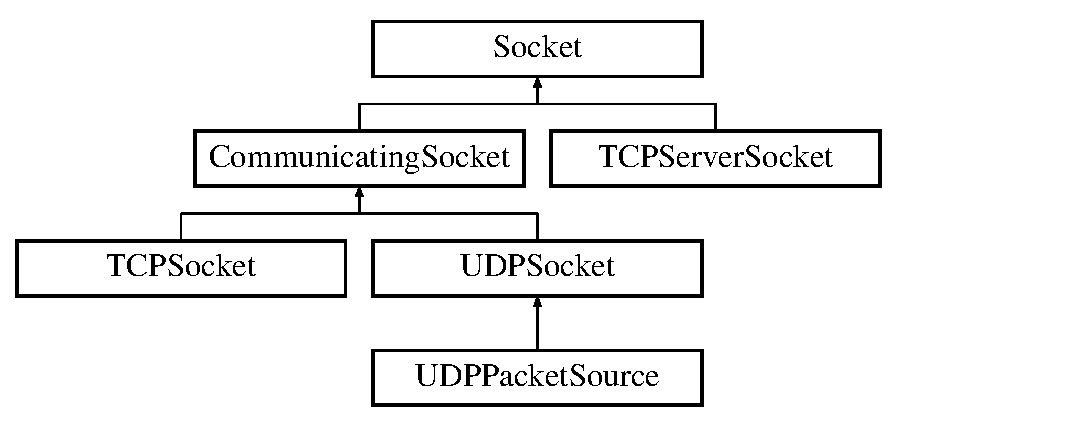
\includegraphics[height=4cm]{classSocket}
\end{center}
\end{figure}
\subsection*{Public Member Functions}
\begin{CompactItemize}
\item 
{\bf $\sim$Socket} ()
\item 
string {\bf get\-Local\-Address} ()  throw (Socket\-Exception)
\item 
unsigned short {\bf get\-Local\-Port} ()  throw (Socket\-Exception)
\item 
void {\bf set\-Local\-Port} (unsigned short local\-Port)  throw (Socket\-Exception)
\item 
void {\bf set\-Local\-Address\-And\-Port} (const string \&local\-Address, unsigned short local\-Port=0)  throw (Socket\-Exception)
\end{CompactItemize}
\subsection*{Static Public Member Functions}
\begin{CompactItemize}
\item 
static void {\bf clean\-Up} ()  throw (Socket\-Exception)
\item 
static unsigned short {\bf resolve\-Service} (const string \&service, const string \&protocol=\char`\"{}tcp\char`\"{})
\end{CompactItemize}
\subsection*{Protected Member Functions}
\begin{CompactItemize}
\item 
{\bf Socket} (int type, int protocol)  throw (Socket\-Exception)
\item 
{\bf Socket} (int {\bf sock\-Desc})
\end{CompactItemize}
\subsection*{Protected Attributes}
\begin{CompactItemize}
\item 
int {\bf sock\-Desc}
\end{CompactItemize}
\subsection*{Private Member Functions}
\begin{CompactItemize}
\item 
{\bf Socket} (const {\bf Socket} \&sock)
\item 
void {\bf operator=} (const {\bf Socket} \&sock)
\end{CompactItemize}


\subsection{Detailed Description}
Base class representing basic communication endpoint 



\subsection{Constructor \& Destructor Documentation}
\index{Socket@{Socket}!~Socket@{$\sim$Socket}}
\index{~Socket@{$\sim$Socket}!Socket@{Socket}}
\subsubsection{\setlength{\rightskip}{0pt plus 5cm}Socket::$\sim$Socket ()}\label{classSocket_eac4eb6379a543d38ed88977d3b6630a}


Close and deallocate this socket \index{Socket@{Socket}!Socket@{Socket}}
\index{Socket@{Socket}!Socket@{Socket}}
\subsubsection{\setlength{\rightskip}{0pt plus 5cm}Socket::Socket (const {\bf Socket} \& {\em sock})\hspace{0.3cm}{\tt  [private]}}\label{classSocket_656389d58fa00729ff70c4e159623f5c}


\index{Socket@{Socket}!Socket@{Socket}}
\index{Socket@{Socket}!Socket@{Socket}}
\subsubsection{\setlength{\rightskip}{0pt plus 5cm}Socket::Socket (int {\em type}, int {\em protocol})  throw ({\bf Socket\-Exception})\hspace{0.3cm}{\tt  [protected]}}\label{classSocket_53e00027bab2125a2b407914c6148589}


\index{Socket@{Socket}!Socket@{Socket}}
\index{Socket@{Socket}!Socket@{Socket}}
\subsubsection{\setlength{\rightskip}{0pt plus 5cm}Socket::Socket (int {\em sock\-Desc})\hspace{0.3cm}{\tt  [protected]}}\label{classSocket_6a2609eef6559336a595a336f138d395}




\subsection{Member Function Documentation}
\index{Socket@{Socket}!getLocalAddress@{getLocalAddress}}
\index{getLocalAddress@{getLocalAddress}!Socket@{Socket}}
\subsubsection{\setlength{\rightskip}{0pt plus 5cm}string Socket::get\-Local\-Address ()  throw ({\bf Socket\-Exception})}\label{classSocket_0fca07bdfa97874fba1a17995ed7cda3}


Get the local address \begin{Desc}
\item[Returns:]local address of socket \end{Desc}
\begin{Desc}
\item[Exceptions:]
\begin{description}
\item[{\em \doxyref{Socket\-Exception}{p.}{classSocketException}}]thrown if fetch fails \end{description}
\end{Desc}
\index{Socket@{Socket}!getLocalPort@{getLocalPort}}
\index{getLocalPort@{getLocalPort}!Socket@{Socket}}
\subsubsection{\setlength{\rightskip}{0pt plus 5cm}unsigned short Socket::get\-Local\-Port ()  throw ({\bf Socket\-Exception})}\label{classSocket_e01143b667d69483a2f53d0f4ce7eeed}


Get the local port \begin{Desc}
\item[Returns:]local port of socket \end{Desc}
\begin{Desc}
\item[Exceptions:]
\begin{description}
\item[{\em \doxyref{Socket\-Exception}{p.}{classSocketException}}]thrown if fetch fails \end{description}
\end{Desc}
\index{Socket@{Socket}!setLocalPort@{setLocalPort}}
\index{setLocalPort@{setLocalPort}!Socket@{Socket}}
\subsubsection{\setlength{\rightskip}{0pt plus 5cm}void Socket::set\-Local\-Port (unsigned short {\em local\-Port})  throw ({\bf Socket\-Exception})}\label{classSocket_773fe4a35146002de76952e16fdebcfa}


Set the local port to the specified port and the local address to any interface \begin{Desc}
\item[Parameters:]
\begin{description}
\item[{\em local\-Port}]local port \end{description}
\end{Desc}
\begin{Desc}
\item[Exceptions:]
\begin{description}
\item[{\em \doxyref{Socket\-Exception}{p.}{classSocketException}}]thrown if setting local port fails \end{description}
\end{Desc}
\index{Socket@{Socket}!setLocalAddressAndPort@{setLocalAddressAndPort}}
\index{setLocalAddressAndPort@{setLocalAddressAndPort}!Socket@{Socket}}
\subsubsection{\setlength{\rightskip}{0pt plus 5cm}void Socket::set\-Local\-Address\-And\-Port (const string \& {\em local\-Address}, unsigned short {\em local\-Port} = {\tt 0})  throw ({\bf Socket\-Exception})}\label{classSocket_a6b986410bc2e606ba27d01fa7cb8836}


Set the local port to the specified port and the local address to the specified address. If you omit the port, a random port will be selected. \begin{Desc}
\item[Parameters:]
\begin{description}
\item[{\em local\-Address}]local address \item[{\em local\-Port}]local port \end{description}
\end{Desc}
\begin{Desc}
\item[Exceptions:]
\begin{description}
\item[{\em \doxyref{Socket\-Exception}{p.}{classSocketException}}]thrown if setting local port or address fails \end{description}
\end{Desc}
\index{Socket@{Socket}!cleanUp@{cleanUp}}
\index{cleanUp@{cleanUp}!Socket@{Socket}}
\subsubsection{\setlength{\rightskip}{0pt plus 5cm}void Socket::clean\-Up ()  throw ({\bf Socket\-Exception})\hspace{0.3cm}{\tt  [static]}}\label{classSocket_c5060aeb501044044351d5a85b3fc95f}


If Win\-Sock, unload the Win\-Sock DLLs; otherwise do nothing. We ignore this in our sample client code but include it in the library for completeness. If you are running on Windows and you are concerned about DLL resource consumption, call this after you are done with all \doxyref{Socket}{p.}{classSocket} instances. If you execute this on Windows while some instance of \doxyref{Socket}{p.}{classSocket} exists, you are toast. For portability of client code, this is an empty function on non-Windows platforms so you can always include it. \begin{Desc}
\item[Parameters:]
\begin{description}
\item[{\em buffer}]buffer to receive the data \item[{\em buffer\-Len}]maximum number of bytes to read into buffer \end{description}
\end{Desc}
\begin{Desc}
\item[Returns:]number of bytes read, 0 for EOF, and -1 for error \end{Desc}
\begin{Desc}
\item[Exceptions:]
\begin{description}
\item[{\em \doxyref{Socket\-Exception}{p.}{classSocketException}}]thrown Win\-Sock clean up fails \end{description}
\end{Desc}
\index{Socket@{Socket}!resolveService@{resolveService}}
\index{resolveService@{resolveService}!Socket@{Socket}}
\subsubsection{\setlength{\rightskip}{0pt plus 5cm}unsigned short Socket::resolve\-Service (const string \& {\em service}, const string \& {\em protocol} = {\tt \char`\"{}tcp\char`\"{}})\hspace{0.3cm}{\tt  [static]}}\label{classSocket_982c63b25c5b756321a74074a275adbc}


Resolve the specified service for the specified protocol to the corresponding port number in host byte order \begin{Desc}
\item[Parameters:]
\begin{description}
\item[{\em service}]service to resolve (e.g., \char`\"{}http\char`\"{}) \item[{\em protocol}]protocol of service to resolve. Default is \char`\"{}tcp\char`\"{}. \end{description}
\end{Desc}
\index{Socket@{Socket}!operator=@{operator=}}
\index{operator=@{operator=}!Socket@{Socket}}
\subsubsection{\setlength{\rightskip}{0pt plus 5cm}void Socket::operator= (const {\bf Socket} \& {\em sock})\hspace{0.3cm}{\tt  [private]}}\label{classSocket_1ef8f4c222c32756c8b1537323702df8}




\subsection{Member Data Documentation}
\index{Socket@{Socket}!sockDesc@{sockDesc}}
\index{sockDesc@{sockDesc}!Socket@{Socket}}
\subsubsection{\setlength{\rightskip}{0pt plus 5cm}int {\bf Socket::sock\-Desc}\hspace{0.3cm}{\tt  [protected]}}\label{classSocket_d5704d2fdfb062139e1f88831617bbfb}




The documentation for this class was generated from the following files:\begin{CompactItemize}
\item 
{\bf Practical\-Socket.h}\item 
{\bf Practical\-Socket.cpp}\end{CompactItemize}

\section{Socket\-Exception Class Reference}
\label{classSocketException}\index{SocketException@{SocketException}}
{\tt \#include $<$Practical\-Socket.h$>$}

\subsection*{Public Member Functions}
\begin{CompactItemize}
\item 
{\bf Socket\-Exception} (const string \&message, bool incl\-Sys\-Msg=false)  throw ()
\item 
{\bf $\sim$Socket\-Exception} ()  throw ()
\item 
const char $\ast$ {\bf what} () const  throw ()
\end{CompactItemize}
\subsection*{Private Attributes}
\begin{CompactItemize}
\item 
string {\bf user\-Message}
\end{CompactItemize}


\subsection{Detailed Description}
Signals a problem with the execution of a socket call. 



\subsection{Constructor \& Destructor Documentation}
\index{SocketException@{Socket\-Exception}!SocketException@{SocketException}}
\index{SocketException@{SocketException}!SocketException@{Socket\-Exception}}
\subsubsection{\setlength{\rightskip}{0pt plus 5cm}Socket\-Exception::Socket\-Exception (const string \& {\em message}, bool {\em incl\-Sys\-Msg} = {\tt false})  throw ()}\label{classSocketException_bb5bcecd9d9e20868c237ec5a82cf5c3}


Construct a \doxyref{Socket\-Exception}{p.}{classSocketException} with a explanatory message. \begin{Desc}
\item[Parameters:]
\begin{description}
\item[{\em message}]explanatory message \item[{\em inc\-Sys\-Msg}]true if system message (from strerror(errno)) should be postfixed to the user provided message \end{description}
\end{Desc}
\index{SocketException@{Socket\-Exception}!~SocketException@{$\sim$SocketException}}
\index{~SocketException@{$\sim$SocketException}!SocketException@{Socket\-Exception}}
\subsubsection{\setlength{\rightskip}{0pt plus 5cm}Socket\-Exception::$\sim$Socket\-Exception ()  throw ()}\label{classSocketException_659557c899329aea01977c980c4db9b9}


Provided just to guarantee that no exceptions are thrown. 

\subsection{Member Function Documentation}
\index{SocketException@{Socket\-Exception}!what@{what}}
\index{what@{what}!SocketException@{Socket\-Exception}}
\subsubsection{\setlength{\rightskip}{0pt plus 5cm}const char $\ast$ Socket\-Exception::what () const  throw ()}\label{classSocketException_534b0625abe62cad2bae94758aa6eb42}


Get the exception message \begin{Desc}
\item[Returns:]exception message \end{Desc}


\subsection{Member Data Documentation}
\index{SocketException@{Socket\-Exception}!userMessage@{userMessage}}
\index{userMessage@{userMessage}!SocketException@{Socket\-Exception}}
\subsubsection{\setlength{\rightskip}{0pt plus 5cm}string {\bf Socket\-Exception::user\-Message}\hspace{0.3cm}{\tt  [private]}}\label{classSocketException_dcfeba6d4ce5754b48ae9d37b07a7e87}




The documentation for this class was generated from the following files:\begin{CompactItemize}
\item 
{\bf Practical\-Socket.h}\item 
{\bf Practical\-Socket.cpp}\end{CompactItemize}

\section{TCPServer\-Socket Class Reference}
\label{classTCPServerSocket}\index{TCPServerSocket@{TCPServerSocket}}
{\tt \#include $<$Practical\-Socket.h$>$}

Inheritance diagram for TCPServer\-Socket::\begin{figure}[H]
\begin{center}
\leavevmode
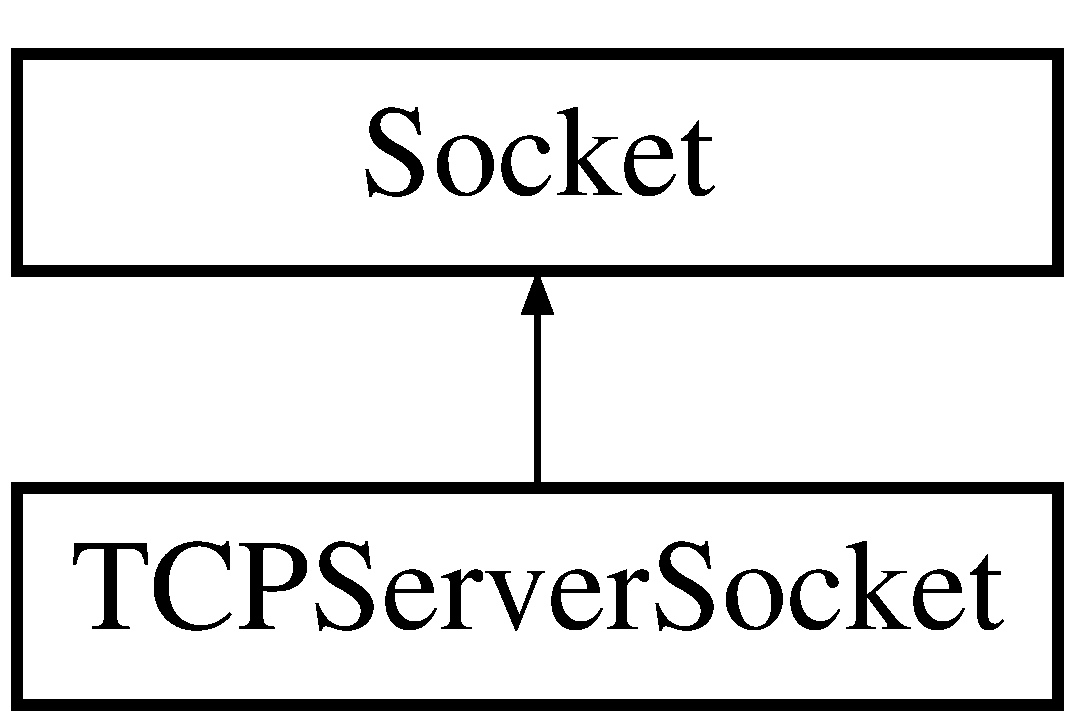
\includegraphics[height=2cm]{classTCPServerSocket}
\end{center}
\end{figure}
\subsection*{Public Member Functions}
\begin{CompactItemize}
\item 
{\bf TCPServer\-Socket} (unsigned short local\-Port, int queue\-Len=5)  throw (Socket\-Exception)
\item 
{\bf TCPServer\-Socket} (const string \&local\-Address, unsigned short local\-Port, int queue\-Len=5)  throw (Socket\-Exception)
\item 
{\bf TCPSocket} $\ast$ {\bf accept} ()  throw (Socket\-Exception)
\end{CompactItemize}
\subsection*{Private Member Functions}
\begin{CompactItemize}
\item 
void {\bf set\-Listen} (int queue\-Len)  throw (Socket\-Exception)
\end{CompactItemize}


\subsection{Detailed Description}
TCP socket class for servers 



\subsection{Constructor \& Destructor Documentation}
\index{TCPServerSocket@{TCPServer\-Socket}!TCPServerSocket@{TCPServerSocket}}
\index{TCPServerSocket@{TCPServerSocket}!TCPServerSocket@{TCPServer\-Socket}}
\subsubsection{\setlength{\rightskip}{0pt plus 5cm}TCPServer\-Socket::TCPServer\-Socket (unsigned short {\em local\-Port}, int {\em queue\-Len} = {\tt 5})  throw ({\bf Socket\-Exception})}\label{classTCPServerSocket_e559a3154527d09fe14a8e5ee1f53d7a}


Construct a TCP socket for use with a server, accepting connections on the specified port on any interface \begin{Desc}
\item[Parameters:]
\begin{description}
\item[{\em local\-Port}]local port of server socket, a value of zero will give a system-assigned unused port \item[{\em queue\-Len}]maximum queue length for outstanding connection requests (default 5) \end{description}
\end{Desc}
\begin{Desc}
\item[Exceptions:]
\begin{description}
\item[{\em \doxyref{Socket\-Exception}{p.}{classSocketException}}]thrown if unable to create TCP server socket \end{description}
\end{Desc}
\index{TCPServerSocket@{TCPServer\-Socket}!TCPServerSocket@{TCPServerSocket}}
\index{TCPServerSocket@{TCPServerSocket}!TCPServerSocket@{TCPServer\-Socket}}
\subsubsection{\setlength{\rightskip}{0pt plus 5cm}TCPServer\-Socket::TCPServer\-Socket (const string \& {\em local\-Address}, unsigned short {\em local\-Port}, int {\em queue\-Len} = {\tt 5})  throw ({\bf Socket\-Exception})}\label{classTCPServerSocket_3908fecb1b038f7c14fcc7726f54d01d}


Construct a TCP socket for use with a server, accepting connections on the specified port on the interface specified by the given address \begin{Desc}
\item[Parameters:]
\begin{description}
\item[{\em local\-Address}]local interface (address) of server socket \item[{\em local\-Port}]local port of server socket \item[{\em queue\-Len}]maximum queue length for outstanding connection requests (default 5) \end{description}
\end{Desc}
\begin{Desc}
\item[Exceptions:]
\begin{description}
\item[{\em \doxyref{Socket\-Exception}{p.}{classSocketException}}]thrown if unable to create TCP server socket \end{description}
\end{Desc}


\subsection{Member Function Documentation}
\index{TCPServerSocket@{TCPServer\-Socket}!accept@{accept}}
\index{accept@{accept}!TCPServerSocket@{TCPServer\-Socket}}
\subsubsection{\setlength{\rightskip}{0pt plus 5cm}{\bf TCPSocket} $\ast$ TCPServer\-Socket::accept ()  throw ({\bf Socket\-Exception})}\label{classTCPServerSocket_1d161137e1b069de7a7bfc14d3f8212c}


Blocks until a new connection is established on this socket or error \begin{Desc}
\item[Returns:]new connection socket \end{Desc}
\begin{Desc}
\item[Exceptions:]
\begin{description}
\item[{\em \doxyref{Socket\-Exception}{p.}{classSocketException}}]thrown if attempt to accept a new connection fails \end{description}
\end{Desc}
\index{TCPServerSocket@{TCPServer\-Socket}!setListen@{setListen}}
\index{setListen@{setListen}!TCPServerSocket@{TCPServer\-Socket}}
\subsubsection{\setlength{\rightskip}{0pt plus 5cm}void TCPServer\-Socket::set\-Listen (int {\em queue\-Len})  throw ({\bf Socket\-Exception})\hspace{0.3cm}{\tt  [private]}}\label{classTCPServerSocket_1f39a2e6721ab62d8875a234eb300bab}




The documentation for this class was generated from the following files:\begin{CompactItemize}
\item 
{\bf Practical\-Socket.h}\item 
{\bf Practical\-Socket.cpp}\end{CompactItemize}

\section{TCPSocket Class Reference}
\label{classTCPSocket}\index{TCPSocket@{TCPSocket}}
{\tt \#include $<$Practical\-Socket.h$>$}

Inheritance diagram for TCPSocket::\begin{figure}[H]
\begin{center}
\leavevmode
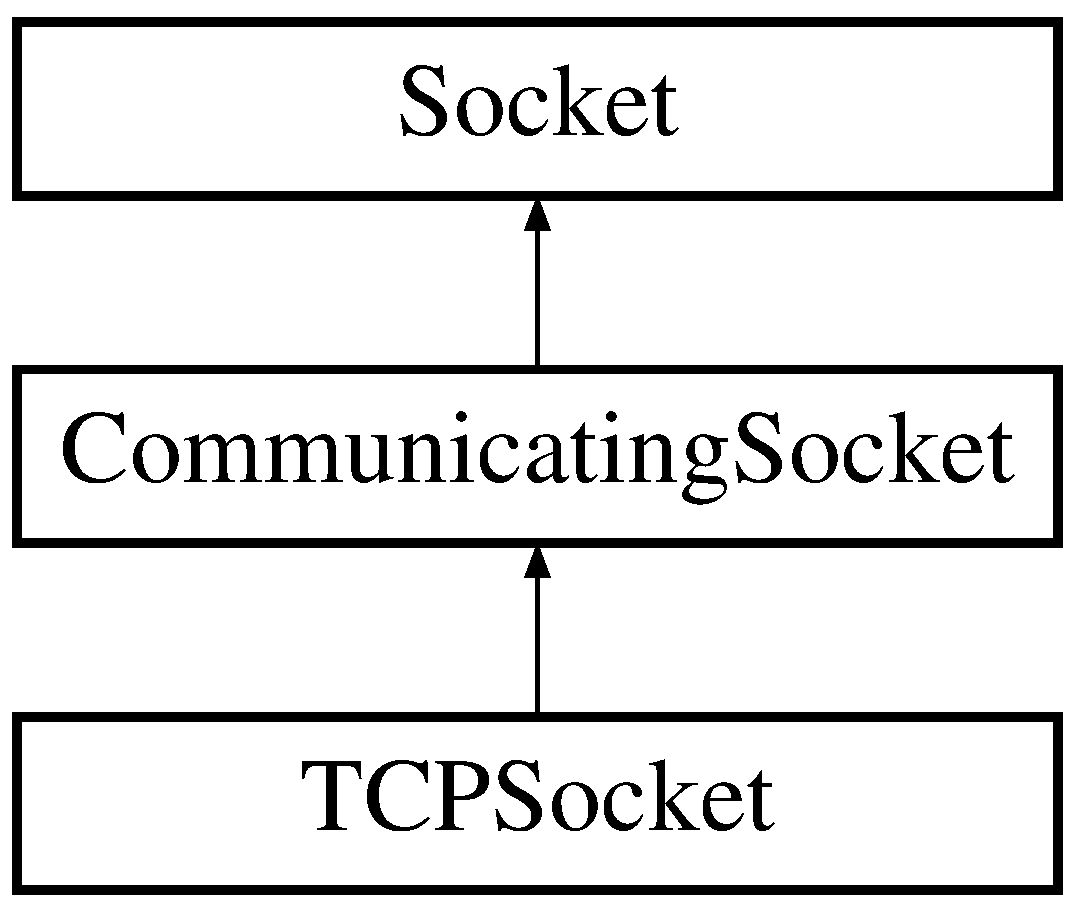
\includegraphics[height=3cm]{classTCPSocket}
\end{center}
\end{figure}
\subsection*{Public Member Functions}
\begin{CompactItemize}
\item 
{\bf TCPSocket} ()  throw (Socket\-Exception)
\item 
{\bf TCPSocket} (const string \&foreign\-Address, unsigned short foreign\-Port)  throw (Socket\-Exception)
\end{CompactItemize}
\subsection*{Private Member Functions}
\begin{CompactItemize}
\item 
{\bf TCPSocket} (int new\-Conn\-SD)
\end{CompactItemize}
\subsection*{Friends}
\begin{CompactItemize}
\item 
class {\bf TCPServer\-Socket}
\end{CompactItemize}


\subsection{Detailed Description}
TCP socket for communication with other TCP sockets 



\subsection{Constructor \& Destructor Documentation}
\index{TCPSocket@{TCPSocket}!TCPSocket@{TCPSocket}}
\index{TCPSocket@{TCPSocket}!TCPSocket@{TCPSocket}}
\subsubsection{\setlength{\rightskip}{0pt plus 5cm}TCPSocket::TCPSocket ()  throw ({\bf Socket\-Exception})}\label{classTCPSocket_7a50427a401d1a6f3209d51818bad901}


Construct a TCP socket with no connection \begin{Desc}
\item[Exceptions:]
\begin{description}
\item[{\em \doxyref{Socket\-Exception}{p.}{classSocketException}}]thrown if unable to create TCP socket \end{description}
\end{Desc}
\index{TCPSocket@{TCPSocket}!TCPSocket@{TCPSocket}}
\index{TCPSocket@{TCPSocket}!TCPSocket@{TCPSocket}}
\subsubsection{\setlength{\rightskip}{0pt plus 5cm}TCPSocket::TCPSocket (const string \& {\em foreign\-Address}, unsigned short {\em foreign\-Port})  throw ({\bf Socket\-Exception})}\label{classTCPSocket_7b246b66f6dc3246ab2777b771e5f917}


Construct a TCP socket with a connection to the given foreign address and port \begin{Desc}
\item[Parameters:]
\begin{description}
\item[{\em foreign\-Address}]foreign address (IP address or name) \item[{\em foreign\-Port}]foreign port \end{description}
\end{Desc}
\begin{Desc}
\item[Exceptions:]
\begin{description}
\item[{\em \doxyref{Socket\-Exception}{p.}{classSocketException}}]thrown if unable to create TCP socket \end{description}
\end{Desc}
\index{TCPSocket@{TCPSocket}!TCPSocket@{TCPSocket}}
\index{TCPSocket@{TCPSocket}!TCPSocket@{TCPSocket}}
\subsubsection{\setlength{\rightskip}{0pt plus 5cm}TCPSocket::TCPSocket (int {\em new\-Conn\-SD})\hspace{0.3cm}{\tt  [private]}}\label{classTCPSocket_4763ac3be0d7d5e143884bef45e351c5}




\subsection{Friends And Related Function Documentation}
\index{TCPSocket@{TCPSocket}!TCPServerSocket@{TCPServerSocket}}
\index{TCPServerSocket@{TCPServerSocket}!TCPSocket@{TCPSocket}}
\subsubsection{\setlength{\rightskip}{0pt plus 5cm}friend class {\bf TCPServer\-Socket}\hspace{0.3cm}{\tt  [friend]}}\label{classTCPSocket_e8bcdc0d25881a17b23e557296236fa9}




The documentation for this class was generated from the following files:\begin{CompactItemize}
\item 
{\bf Practical\-Socket.h}\item 
{\bf Practical\-Socket.cpp}\end{CompactItemize}

\section{Tun\-Device Class Reference}
\label{classTunDevice}\index{TunDevice@{TunDevice}}
{\tt \#include $<$tun\-Device.h$>$}

\subsection*{Public Member Functions}
\begin{CompactItemize}
\item 
{\bf Tun\-Device} (const char $\ast$dev, const char $\ast$dev\_\-type, const char $\ast$ifcfg\_\-lp, const char $\ast$ifcfg\_\-rnmp)
\item 
{\bf $\sim$Tun\-Device} ()
\item 
void {\bf open} ()
\item 
void {\bf close} ()
\item 
bool {\bf is\-Open} ()
\item 
short {\bf read} ({\bf Buffer} \&buf)
\item 
int {\bf write} ({\bf Buffer} \&buf)
\item 
char $\ast$ {\bf get\-Actual\-Name} ()
\item 
{\bf u\_\-int32\_\-t} {\bf get\-Type} ()
\item 
char $\ast$ {\bf get\-Type\-String} ()
\end{CompactItemize}
\subsection*{Static Public Attributes}
\begin{CompactItemize}
\item 
static const {\bf u\_\-int32\_\-t} {\bf TYPE\_\-UNDEF} = 0
\item 
static const {\bf u\_\-int32\_\-t} {\bf TYPE\_\-TUN} = 1
\item 
static const {\bf u\_\-int32\_\-t} {\bf TYPE\_\-TAP} = 2
\end{CompactItemize}
\subsection*{Private Member Functions}
\begin{CompactItemize}
\item 
void {\bf operator=} (const {\bf Tun\-Device} \&src)
\item 
{\bf Tun\-Device} (const {\bf Tun\-Device} \&src)
\end{CompactItemize}
\subsection*{Private Attributes}
\begin{CompactItemize}
\item 
{\bf Mutex} {\bf io\_\-mutex\_\-}
\item 
tuntap $\ast$ {\bf dev\_\-}
\end{CompactItemize}


\subsection{Constructor \& Destructor Documentation}
\index{TunDevice@{Tun\-Device}!TunDevice@{TunDevice}}
\index{TunDevice@{TunDevice}!TunDevice@{Tun\-Device}}
\subsubsection{\setlength{\rightskip}{0pt plus 5cm}Tun\-Device::Tun\-Device (const char $\ast$ {\em dev}, const char $\ast$ {\em dev\_\-type}, const char $\ast$ {\em ifcfg\_\-lp}, const char $\ast$ {\em ifcfg\_\-rnmp})}\label{classTunDevice_d6914bd3a45e03ffe95676ac4420154a}


\index{TunDevice@{Tun\-Device}!~TunDevice@{$\sim$TunDevice}}
\index{~TunDevice@{$\sim$TunDevice}!TunDevice@{Tun\-Device}}
\subsubsection{\setlength{\rightskip}{0pt plus 5cm}Tun\-Device::$\sim$Tun\-Device ()}\label{classTunDevice_2c6196d270bf4d0e99ff4f860391faed}


\index{TunDevice@{Tun\-Device}!TunDevice@{TunDevice}}
\index{TunDevice@{TunDevice}!TunDevice@{Tun\-Device}}
\subsubsection{\setlength{\rightskip}{0pt plus 5cm}Tun\-Device::Tun\-Device (const {\bf Tun\-Device} \& {\em src})\hspace{0.3cm}{\tt  [private]}}\label{classTunDevice_4587b54228b4240334ad4614211df394}




\subsection{Member Function Documentation}
\index{TunDevice@{Tun\-Device}!open@{open}}
\index{open@{open}!TunDevice@{Tun\-Device}}
\subsubsection{\setlength{\rightskip}{0pt plus 5cm}void Tun\-Device::open ()}\label{classTunDevice_323ddcfd4ac60d0dbfe6ebb5bbb9a323}


\index{TunDevice@{Tun\-Device}!close@{close}}
\index{close@{close}!TunDevice@{Tun\-Device}}
\subsubsection{\setlength{\rightskip}{0pt plus 5cm}void Tun\-Device::close ()}\label{classTunDevice_13986e13fe28da6c917293c40effb902}


\index{TunDevice@{Tun\-Device}!isOpen@{isOpen}}
\index{isOpen@{isOpen}!TunDevice@{Tun\-Device}}
\subsubsection{\setlength{\rightskip}{0pt plus 5cm}bool Tun\-Device::is\-Open ()}\label{classTunDevice_f63f3331789f043e44eb435b78c815b2}


\index{TunDevice@{Tun\-Device}!read@{read}}
\index{read@{read}!TunDevice@{Tun\-Device}}
\subsubsection{\setlength{\rightskip}{0pt plus 5cm}short Tun\-Device::read ({\bf Buffer} \& {\em buf})}\label{classTunDevice_553498887edc92f7b7e31e3bf04fb8fb}


\index{TunDevice@{Tun\-Device}!write@{write}}
\index{write@{write}!TunDevice@{Tun\-Device}}
\subsubsection{\setlength{\rightskip}{0pt plus 5cm}int Tun\-Device::write ({\bf Buffer} \& {\em buf})}\label{classTunDevice_958bc73a627cc5d404ed87204547134d}


\index{TunDevice@{Tun\-Device}!getActualName@{getActualName}}
\index{getActualName@{getActualName}!TunDevice@{Tun\-Device}}
\subsubsection{\setlength{\rightskip}{0pt plus 5cm}char $\ast$ Tun\-Device::get\-Actual\-Name ()}\label{classTunDevice_e02f8972f75b11b69280fba9b6649cab}


\index{TunDevice@{Tun\-Device}!getType@{getType}}
\index{getType@{getType}!TunDevice@{Tun\-Device}}
\subsubsection{\setlength{\rightskip}{0pt plus 5cm}{\bf u\_\-int32\_\-t} Tun\-Device::get\-Type ()}\label{classTunDevice_b57512464007681dcc92820adb3deb0f}


\index{TunDevice@{Tun\-Device}!getTypeString@{getTypeString}}
\index{getTypeString@{getTypeString}!TunDevice@{Tun\-Device}}
\subsubsection{\setlength{\rightskip}{0pt plus 5cm}char $\ast$ Tun\-Device::get\-Type\-String ()}\label{classTunDevice_0cecbc6a7e58d294dd005e7d523173bd}


\index{TunDevice@{Tun\-Device}!operator=@{operator=}}
\index{operator=@{operator=}!TunDevice@{Tun\-Device}}
\subsubsection{\setlength{\rightskip}{0pt plus 5cm}void Tun\-Device::operator= (const {\bf Tun\-Device} \& {\em src})\hspace{0.3cm}{\tt  [private]}}\label{classTunDevice_de33e9a7a951b43f2f7e24d8fe9c311e}




\subsection{Member Data Documentation}
\index{TunDevice@{Tun\-Device}!TYPE_UNDEF@{TYPE\_\-UNDEF}}
\index{TYPE_UNDEF@{TYPE\_\-UNDEF}!TunDevice@{Tun\-Device}}
\subsubsection{\setlength{\rightskip}{0pt plus 5cm}const {\bf u\_\-int32\_\-t} {\bf Tun\-Device::TYPE\_\-UNDEF} = 0\hspace{0.3cm}{\tt  [static]}}\label{classTunDevice_ec146b27c7755747c1cc1511e4482875}


\index{TunDevice@{Tun\-Device}!TYPE_TUN@{TYPE\_\-TUN}}
\index{TYPE_TUN@{TYPE\_\-TUN}!TunDevice@{Tun\-Device}}
\subsubsection{\setlength{\rightskip}{0pt plus 5cm}const {\bf u\_\-int32\_\-t} {\bf Tun\-Device::TYPE\_\-TUN} = 1\hspace{0.3cm}{\tt  [static]}}\label{classTunDevice_ea416d7f03ef22bf1d166d33b47fd993}


\index{TunDevice@{Tun\-Device}!TYPE_TAP@{TYPE\_\-TAP}}
\index{TYPE_TAP@{TYPE\_\-TAP}!TunDevice@{Tun\-Device}}
\subsubsection{\setlength{\rightskip}{0pt plus 5cm}const {\bf u\_\-int32\_\-t} {\bf Tun\-Device::TYPE\_\-TAP} = 2\hspace{0.3cm}{\tt  [static]}}\label{classTunDevice_b4ce6b158bbe4fe051b6fea8cd3d6cd3}


\index{TunDevice@{Tun\-Device}!io_mutex_@{io\_\-mutex\_\-}}
\index{io_mutex_@{io\_\-mutex\_\-}!TunDevice@{Tun\-Device}}
\subsubsection{\setlength{\rightskip}{0pt plus 5cm}{\bf Mutex} {\bf Tun\-Device::io\_\-mutex\_\-}\hspace{0.3cm}{\tt  [private]}}\label{classTunDevice_e130228e28996e644d2013089e704d4c}


\index{TunDevice@{Tun\-Device}!dev_@{dev\_\-}}
\index{dev_@{dev\_\-}!TunDevice@{Tun\-Device}}
\subsubsection{\setlength{\rightskip}{0pt plus 5cm}struct tuntap$\ast$ {\bf Tun\-Device::dev\_\-}\hspace{0.3cm}{\tt  [private]}}\label{classTunDevice_239c85381dfcf1776303778d1784df51}




The documentation for this class was generated from the following files:\begin{CompactItemize}
\item 
{\bf tun\-Device.h}\item 
{\bf tun\-Device.cpp}\end{CompactItemize}

\section{UDPPacket\-Source Class Reference}
\label{classUDPPacketSource}\index{UDPPacketSource@{UDPPacketSource}}
{\tt \#include $<$packet\-Source.h$>$}

Inheritance diagram for UDPPacket\-Source::\begin{figure}[H]
\begin{center}
\leavevmode
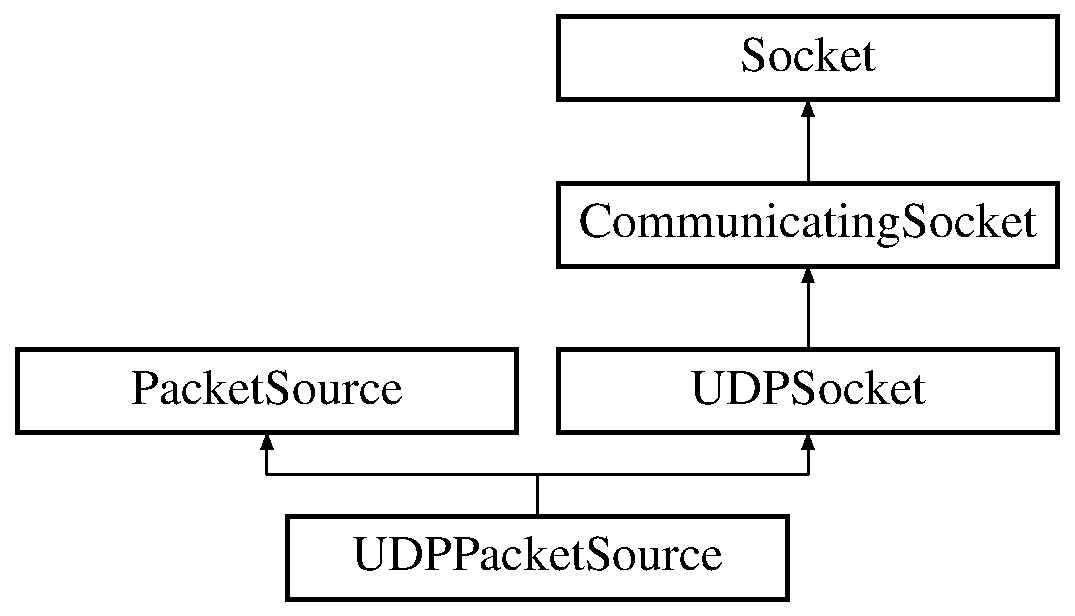
\includegraphics[height=4cm]{classUDPPacketSource}
\end{center}
\end{figure}
\subsection*{Public Member Functions}
\begin{CompactItemize}
\item 
{\bf UDPPacket\-Source} ()
\item 
{\bf UDPPacket\-Source} ({\bf u\_\-int16\_\-t} port)
\item 
{\bf UDPPacket\-Source} (std::string localaddr, {\bf u\_\-int16\_\-t} port)
\item 
{\bf u\_\-int32\_\-t} {\bf recv} ({\bf Buffer} \&buf, std::string \&addr, {\bf u\_\-int16\_\-t} \&port)
\item 
void {\bf send} ({\bf Buffer} \&buf, std::string addr, {\bf u\_\-int16\_\-t} port)
\end{CompactItemize}


\subsection{Constructor \& Destructor Documentation}
\index{UDPPacketSource@{UDPPacket\-Source}!UDPPacketSource@{UDPPacketSource}}
\index{UDPPacketSource@{UDPPacketSource}!UDPPacketSource@{UDPPacket\-Source}}
\subsubsection{\setlength{\rightskip}{0pt plus 5cm}UDPPacket\-Source::UDPPacket\-Source ()}\label{classUDPPacketSource_1dda248d4d7b03cb8301557271abc40e}


\index{UDPPacketSource@{UDPPacket\-Source}!UDPPacketSource@{UDPPacketSource}}
\index{UDPPacketSource@{UDPPacketSource}!UDPPacketSource@{UDPPacket\-Source}}
\subsubsection{\setlength{\rightskip}{0pt plus 5cm}UDPPacket\-Source::UDPPacket\-Source ({\bf u\_\-int16\_\-t} {\em port})}\label{classUDPPacketSource_b9fd5944db99fd0f89c12b0d74ba5e74}


\index{UDPPacketSource@{UDPPacket\-Source}!UDPPacketSource@{UDPPacketSource}}
\index{UDPPacketSource@{UDPPacketSource}!UDPPacketSource@{UDPPacket\-Source}}
\subsubsection{\setlength{\rightskip}{0pt plus 5cm}UDPPacket\-Source::UDPPacket\-Source (std::string {\em localaddr}, {\bf u\_\-int16\_\-t} {\em port})}\label{classUDPPacketSource_1cc870353b550b79f9161cfac41f26fa}




\subsection{Member Function Documentation}
\index{UDPPacketSource@{UDPPacket\-Source}!recv@{recv}}
\index{recv@{recv}!UDPPacketSource@{UDPPacket\-Source}}
\subsubsection{\setlength{\rightskip}{0pt plus 5cm}{\bf u\_\-int32\_\-t} UDPPacket\-Source::recv ({\bf Buffer} \& {\em buf}, std::string \& {\em addr}, {\bf u\_\-int16\_\-t} \& {\em port})\hspace{0.3cm}{\tt  [virtual]}}\label{classUDPPacketSource_a1f7daded0f9ead5599160bae9317eb8}




Implements {\bf Packet\-Source} \doxyref{}{p.}{classPacketSource_95901be715656540a7273c6c0dc1234e}.\index{UDPPacketSource@{UDPPacket\-Source}!send@{send}}
\index{send@{send}!UDPPacketSource@{UDPPacket\-Source}}
\subsubsection{\setlength{\rightskip}{0pt plus 5cm}void UDPPacket\-Source::send ({\bf Buffer} \& {\em buf}, std::string {\em addr}, {\bf u\_\-int16\_\-t} {\em port})\hspace{0.3cm}{\tt  [virtual]}}\label{classUDPPacketSource_376a3b0c861aeb7561e8a9f6866292b9}




Implements {\bf Packet\-Source} \doxyref{}{p.}{classPacketSource_ffc5eb2c89d1395443432c3cc6b7898b}.

The documentation for this class was generated from the following files:\begin{CompactItemize}
\item 
{\bf packet\-Source.h}\item 
{\bf packet\-Source.cpp}\end{CompactItemize}

\section{UDPSocket Class Reference}
\label{classUDPSocket}\index{UDPSocket@{UDPSocket}}
{\tt \#include $<$Practical\-Socket.h$>$}

Inheritance diagram for UDPSocket::\begin{figure}[H]
\begin{center}
\leavevmode
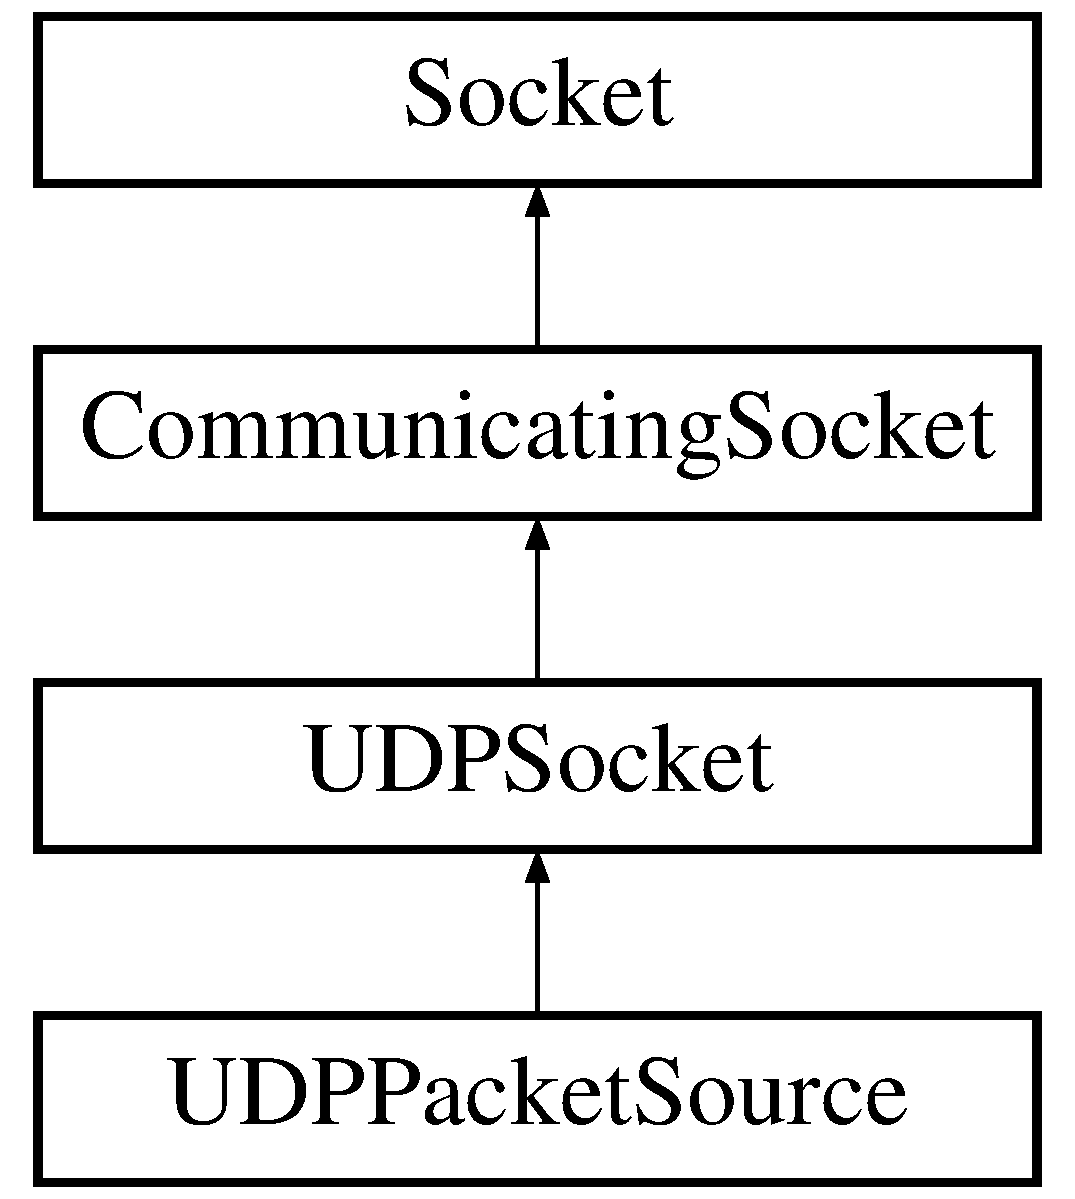
\includegraphics[height=4cm]{classUDPSocket}
\end{center}
\end{figure}
\subsection*{Public Member Functions}
\begin{CompactItemize}
\item 
{\bf UDPSocket} ()  throw (Socket\-Exception)
\item 
{\bf UDPSocket} (unsigned short local\-Port)  throw (Socket\-Exception)
\item 
{\bf UDPSocket} (const string \&local\-Address, unsigned short local\-Port)  throw (Socket\-Exception)
\item 
void {\bf disconnect} ()  throw (Socket\-Exception)
\item 
void {\bf send\-To} (const void $\ast$buffer, int buffer\-Len, const string \&foreign\-Address, unsigned short foreign\-Port)  throw (Socket\-Exception)
\item 
int {\bf recv\-From} (void $\ast$buffer, int buffer\-Len, string \&source\-Address, unsigned short \&source\-Port)  throw (Socket\-Exception)
\item 
void {\bf set\-Multicast\-TTL} (unsigned char multicast\-TTL)  throw (Socket\-Exception)
\item 
void {\bf join\-Group} (const string \&multicast\-Group)  throw (Socket\-Exception)
\item 
void {\bf leave\-Group} (const string \&multicast\-Group)  throw (Socket\-Exception)
\end{CompactItemize}
\subsection*{Private Member Functions}
\begin{CompactItemize}
\item 
void {\bf set\-Broadcast} ()
\end{CompactItemize}


\subsection{Detailed Description}
UDP socket class 



\subsection{Constructor \& Destructor Documentation}
\index{UDPSocket@{UDPSocket}!UDPSocket@{UDPSocket}}
\index{UDPSocket@{UDPSocket}!UDPSocket@{UDPSocket}}
\subsubsection{\setlength{\rightskip}{0pt plus 5cm}UDPSocket::UDPSocket ()  throw ({\bf Socket\-Exception})}\label{classUDPSocket_4f86f3023f5a08f6355802599a10e100}


Construct a UDP socket \begin{Desc}
\item[Exceptions:]
\begin{description}
\item[{\em \doxyref{Socket\-Exception}{p.}{classSocketException}}]thrown if unable to create UDP socket \end{description}
\end{Desc}
\index{UDPSocket@{UDPSocket}!UDPSocket@{UDPSocket}}
\index{UDPSocket@{UDPSocket}!UDPSocket@{UDPSocket}}
\subsubsection{\setlength{\rightskip}{0pt plus 5cm}UDPSocket::UDPSocket (unsigned short {\em local\-Port})  throw ({\bf Socket\-Exception})}\label{classUDPSocket_14dcb55c4b60b12d4a7fff648cbb825f}


Construct a UDP socket with the given local port \begin{Desc}
\item[Parameters:]
\begin{description}
\item[{\em local\-Port}]local port \end{description}
\end{Desc}
\begin{Desc}
\item[Exceptions:]
\begin{description}
\item[{\em \doxyref{Socket\-Exception}{p.}{classSocketException}}]thrown if unable to create UDP socket \end{description}
\end{Desc}
\index{UDPSocket@{UDPSocket}!UDPSocket@{UDPSocket}}
\index{UDPSocket@{UDPSocket}!UDPSocket@{UDPSocket}}
\subsubsection{\setlength{\rightskip}{0pt plus 5cm}UDPSocket::UDPSocket (const string \& {\em local\-Address}, unsigned short {\em local\-Port})  throw ({\bf Socket\-Exception})}\label{classUDPSocket_f19281c523f15ed30d7d78f09033713d}


Construct a UDP socket with the given local port and address \begin{Desc}
\item[Parameters:]
\begin{description}
\item[{\em local\-Address}]local address \item[{\em local\-Port}]local port \end{description}
\end{Desc}
\begin{Desc}
\item[Exceptions:]
\begin{description}
\item[{\em \doxyref{Socket\-Exception}{p.}{classSocketException}}]thrown if unable to create UDP socket \end{description}
\end{Desc}


\subsection{Member Function Documentation}
\index{UDPSocket@{UDPSocket}!disconnect@{disconnect}}
\index{disconnect@{disconnect}!UDPSocket@{UDPSocket}}
\subsubsection{\setlength{\rightskip}{0pt plus 5cm}void UDPSocket::disconnect ()  throw ({\bf Socket\-Exception})}\label{classUDPSocket_7482e8e61cef160e1a7c0d6ac15c01be}


Unset foreign address and port \begin{Desc}
\item[Returns:]true if disassociation is successful \end{Desc}
\begin{Desc}
\item[Exceptions:]
\begin{description}
\item[{\em \doxyref{Socket\-Exception}{p.}{classSocketException}}]thrown if unable to disconnect UDP socket \end{description}
\end{Desc}
\index{UDPSocket@{UDPSocket}!sendTo@{sendTo}}
\index{sendTo@{sendTo}!UDPSocket@{UDPSocket}}
\subsubsection{\setlength{\rightskip}{0pt plus 5cm}void UDPSocket::send\-To (const void $\ast$ {\em buffer}, int {\em buffer\-Len}, const string \& {\em foreign\-Address}, unsigned short {\em foreign\-Port})  throw ({\bf Socket\-Exception})}\label{classUDPSocket_41a3595e226f273953cbd38618af5d5b}


Send the given buffer as a UDP datagram to the specified address/port \begin{Desc}
\item[Parameters:]
\begin{description}
\item[{\em buffer}]buffer to be written \item[{\em buffer\-Len}]number of bytes to write \item[{\em foreign\-Address}]address (IP address or name) to send to \item[{\em foreign\-Port}]port number to send to \end{description}
\end{Desc}
\begin{Desc}
\item[Returns:]true if send is successful \end{Desc}
\begin{Desc}
\item[Exceptions:]
\begin{description}
\item[{\em \doxyref{Socket\-Exception}{p.}{classSocketException}}]thrown if unable to send datagram \end{description}
\end{Desc}
\index{UDPSocket@{UDPSocket}!recvFrom@{recvFrom}}
\index{recvFrom@{recvFrom}!UDPSocket@{UDPSocket}}
\subsubsection{\setlength{\rightskip}{0pt plus 5cm}int UDPSocket::recv\-From (void $\ast$ {\em buffer}, int {\em buffer\-Len}, string \& {\em source\-Address}, unsigned short \& {\em source\-Port})  throw ({\bf Socket\-Exception})}\label{classUDPSocket_bcd5c064e2496bd8b1888fd4e1b68949}


Read read up to buffer\-Len bytes data from this socket. The given buffer is where the data will be placed \begin{Desc}
\item[Parameters:]
\begin{description}
\item[{\em buffer}]buffer to receive data \item[{\em buffer\-Len}]maximum number of bytes to receive \item[{\em source\-Address}]address of datagram source \item[{\em source\-Port}]port of data source \end{description}
\end{Desc}
\begin{Desc}
\item[Returns:]number of bytes received and -1 for error \end{Desc}
\begin{Desc}
\item[Exceptions:]
\begin{description}
\item[{\em \doxyref{Socket\-Exception}{p.}{classSocketException}}]thrown if unable to receive datagram \end{description}
\end{Desc}
\index{UDPSocket@{UDPSocket}!setMulticastTTL@{setMulticastTTL}}
\index{setMulticastTTL@{setMulticastTTL}!UDPSocket@{UDPSocket}}
\subsubsection{\setlength{\rightskip}{0pt plus 5cm}void UDPSocket::set\-Multicast\-TTL (unsigned char {\em multicast\-TTL})  throw ({\bf Socket\-Exception})}\label{classUDPSocket_4dcfff33b45d1b84b5a602fc6f4a27f8}


Set the multicast TTL \begin{Desc}
\item[Parameters:]
\begin{description}
\item[{\em multicast\-TTL}]multicast TTL \end{description}
\end{Desc}
\begin{Desc}
\item[Exceptions:]
\begin{description}
\item[{\em \doxyref{Socket\-Exception}{p.}{classSocketException}}]thrown if unable to set TTL \end{description}
\end{Desc}
\index{UDPSocket@{UDPSocket}!joinGroup@{joinGroup}}
\index{joinGroup@{joinGroup}!UDPSocket@{UDPSocket}}
\subsubsection{\setlength{\rightskip}{0pt plus 5cm}void UDPSocket::join\-Group (const string \& {\em multicast\-Group})  throw ({\bf Socket\-Exception})}\label{classUDPSocket_1b20c1e8bd49a9bd9b53dd4f1c8d4c11}


Join the specified multicast group \begin{Desc}
\item[Parameters:]
\begin{description}
\item[{\em multicast\-Group}]multicast group address to join \end{description}
\end{Desc}
\begin{Desc}
\item[Exceptions:]
\begin{description}
\item[{\em \doxyref{Socket\-Exception}{p.}{classSocketException}}]thrown if unable to join group \end{description}
\end{Desc}
\index{UDPSocket@{UDPSocket}!leaveGroup@{leaveGroup}}
\index{leaveGroup@{leaveGroup}!UDPSocket@{UDPSocket}}
\subsubsection{\setlength{\rightskip}{0pt plus 5cm}void UDPSocket::leave\-Group (const string \& {\em multicast\-Group})  throw ({\bf Socket\-Exception})}\label{classUDPSocket_78835eaeca8a5ac039b4579c795e3640}


Leave the specified multicast group \begin{Desc}
\item[Parameters:]
\begin{description}
\item[{\em multicast\-Group}]multicast group address to leave \end{description}
\end{Desc}
\begin{Desc}
\item[Exceptions:]
\begin{description}
\item[{\em \doxyref{Socket\-Exception}{p.}{classSocketException}}]thrown if unable to leave group \end{description}
\end{Desc}
\index{UDPSocket@{UDPSocket}!setBroadcast@{setBroadcast}}
\index{setBroadcast@{setBroadcast}!UDPSocket@{UDPSocket}}
\subsubsection{\setlength{\rightskip}{0pt plus 5cm}void UDPSocket::set\-Broadcast ()\hspace{0.3cm}{\tt  [private]}}\label{classUDPSocket_316f08a017aa160643812f3c08734d27}




The documentation for this class was generated from the following files:\begin{CompactItemize}
\item 
{\bf Practical\-Socket.h}\item 
{\bf Practical\-Socket.cpp}\end{CompactItemize}

\chapter{anytun File Documentation}
\section{anytun.cpp File Reference}
\label{anytun_8cpp}\index{anytun.cpp@{anytun.cpp}}
{\tt \#include $<$iostream$>$}\par
{\tt \#include $<$poll.h$>$}\par
{\tt \#include \char`\"{}datatypes.h\char`\"{}}\par
{\tt \#include \char`\"{}log.h\char`\"{}}\par
{\tt \#include \char`\"{}buffer.h\char`\"{}}\par
{\tt \#include \char`\"{}packet.h\char`\"{}}\par
{\tt \#include \char`\"{}cypher.h\char`\"{}}\par
{\tt \#include \char`\"{}key\-Derivation.h\char`\"{}}\par
{\tt \#include \char`\"{}auth\-Algo.h\char`\"{}}\par
{\tt \#include \char`\"{}signal\-Controller.h\char`\"{}}\par
{\tt \#include \char`\"{}packet\-Source.h\char`\"{}}\par
{\tt \#include \char`\"{}tun\-Device.h\char`\"{}}\par
{\tt \#include \char`\"{}options.h\char`\"{}}\par
{\tt \#include \char`\"{}seq\-Window.h\char`\"{}}\par
\subsection*{Classes}
\begin{CompactItemize}
\item 
struct {\bf Param}
\end{CompactItemize}
\subsection*{Defines}
\begin{CompactItemize}
\item 
\#define {\bf PAYLOAD\_\-TYPE\_\-TAP}~0x6558
\item 
\#define {\bf PAYLOAD\_\-TYPE\_\-TUN}~0x0800
\end{CompactItemize}
\subsection*{Functions}
\begin{CompactItemize}
\item 
void $\ast$ {\bf sender} (void $\ast$p)
\item 
void $\ast$ {\bf sync\_\-receiver} (void $\ast$p)
\item 
void $\ast$ {\bf receiver} (void $\ast$p)
\item 
int {\bf main} (int argc, char $\ast$argv[$\,$])
\end{CompactItemize}


\subsection{Define Documentation}
\index{anytun.cpp@{anytun.cpp}!PAYLOAD_TYPE_TAP@{PAYLOAD\_\-TYPE\_\-TAP}}
\index{PAYLOAD_TYPE_TAP@{PAYLOAD\_\-TYPE\_\-TAP}!anytun.cpp@{anytun.cpp}}
\subsubsection{\setlength{\rightskip}{0pt plus 5cm}\#define PAYLOAD\_\-TYPE\_\-TAP~0x6558}\label{anytun_8cpp_f591627e223468579b78887ef91cb0ac}


\index{anytun.cpp@{anytun.cpp}!PAYLOAD_TYPE_TUN@{PAYLOAD\_\-TYPE\_\-TUN}}
\index{PAYLOAD_TYPE_TUN@{PAYLOAD\_\-TYPE\_\-TUN}!anytun.cpp@{anytun.cpp}}
\subsubsection{\setlength{\rightskip}{0pt plus 5cm}\#define PAYLOAD\_\-TYPE\_\-TUN~0x0800}\label{anytun_8cpp_21c6078872dcc3914076daa2c1ec841a}




\subsection{Function Documentation}
\index{anytun.cpp@{anytun.cpp}!main@{main}}
\index{main@{main}!anytun.cpp@{anytun.cpp}}
\subsubsection{\setlength{\rightskip}{0pt plus 5cm}int main (int {\em argc}, char $\ast$ {\em argv}[$\,$])}\label{anytun_8cpp_0ddf1224851353fc92bfbff6f499fa97}


\index{anytun.cpp@{anytun.cpp}!receiver@{receiver}}
\index{receiver@{receiver}!anytun.cpp@{anytun.cpp}}
\subsubsection{\setlength{\rightskip}{0pt plus 5cm}void$\ast$ receiver (void $\ast$ {\em p})}\label{anytun_8cpp_1a93139691e3d8cf8a996c973c5ca0ac}


\index{anytun.cpp@{anytun.cpp}!sender@{sender}}
\index{sender@{sender}!anytun.cpp@{anytun.cpp}}
\subsubsection{\setlength{\rightskip}{0pt plus 5cm}void$\ast$ sender (void $\ast$ {\em p})}\label{anytun_8cpp_0f2bdeb94d90f5229b9e904e592b24fd}


\index{anytun.cpp@{anytun.cpp}!sync_receiver@{sync\_\-receiver}}
\index{sync_receiver@{sync\_\-receiver}!anytun.cpp@{anytun.cpp}}
\subsubsection{\setlength{\rightskip}{0pt plus 5cm}void$\ast$ sync\_\-receiver (void $\ast$ {\em p})}\label{anytun_8cpp_4fd43e7c243b1cc78c583a915dfd4d55}



\section{auth\-Algo.cpp File Reference}
\label{authAlgo_8cpp}\index{authAlgo.cpp@{authAlgo.cpp}}
{\tt \#include \char`\"{}auth\-Algo.h\char`\"{}}\par
{\tt \#include $<$gcrypt.h$>$}\par

\section{auth\-Algo.h File Reference}
\label{authAlgo_8h}\index{authAlgo.h@{authAlgo.h}}
{\tt \#include \char`\"{}datatypes.h\char`\"{}}\par
{\tt \#include \char`\"{}buffer.h\char`\"{}}\par
\subsection*{Classes}
\begin{CompactItemize}
\item 
class {\bf Auth\-Algo}
\item 
class {\bf Null\-Auth\-Algo}
\item 
class {\bf Hmac\-Auth\-Algo}
\end{CompactItemize}

\section{buffer.cpp File Reference}
\label{buffer_8cpp}\index{buffer.cpp@{buffer.cpp}}
{\tt \#include $<$stdexcept$>$}\par
{\tt \#include $<$string$>$}\par
{\tt \#include $<$cstdio$>$}\par
{\tt \#include $<$iostream$>$}\par
{\tt \#include \char`\"{}datatypes.h\char`\"{}}\par
{\tt \#include \char`\"{}buffer.h\char`\"{}}\par

\section{buffer.h File Reference}
\label{buffer_8h}\index{buffer.h@{buffer.h}}
{\tt \#include \char`\"{}datatypes.h\char`\"{}}\par
\subsection*{Classes}
\begin{CompactItemize}
\item 
class {\bf Buffer}
\end{CompactItemize}

\include{connectionList_8cpp}
\include{connectionList_8h}
\include{connectionParam_8cpp}
\include{connectionParam_8h}
\section{cypher.cpp File Reference}
\label{cypher_8cpp}\index{cypher.cpp@{cypher.cpp}}
{\tt \#include $<$stdexcept$>$}\par
{\tt \#include $<$vector$>$}\par
{\tt \#include $<$iostream$>$}\par
{\tt \#include \char`\"{}cypher.h\char`\"{}}\par
{\tt \#include \char`\"{}key\-Derivation.h\char`\"{}}\par
{\tt \#include $<$gcrypt.h$>$}\par

\section{cypher.h File Reference}
\label{cypher_8h}\index{cypher.h@{cypher.h}}
{\tt \#include \char`\"{}datatypes.h\char`\"{}}\par
{\tt \#include \char`\"{}buffer.h\char`\"{}}\par
{\tt \#include $<$gcrypt.h$>$}\par
{\tt \#include $<$string$>$}\par
\subsection*{Classes}
\begin{CompactItemize}
\item 
class {\bf Cypher}
\item 
class {\bf Null\-Cypher}
\item 
class {\bf Aes\-Icm\-Cypher}
\end{CompactItemize}

\section{datatypes.h File Reference}
\label{datatypes_8h}\index{datatypes.h@{datatypes.h}}
\subsection*{Defines}
\begin{CompactItemize}
\item 
\#define {\bf SEQ\_\-NR\_\-T\_\-NTOH}(a)~ntohl(a)
\item 
\#define {\bf SEQ\_\-NR\_\-T\_\-HTON}(a)~htonl(a)
\item 
\#define {\bf SENDER\_\-ID\_\-T\_\-NTOH}(a)~ntohs(a)
\item 
\#define {\bf SENDER\_\-ID\_\-T\_\-HTON}(a)~htons(a)
\item 
\#define {\bf PAYLOAD\_\-TYPE\_\-T\_\-NTOH}(a)~ntohs(a)
\item 
\#define {\bf PAYLOAD\_\-TYPE\_\-T\_\-HTON}(a)~htons(a)
\item 
\#define {\bf AUTH\_\-TAG\_\-T\_\-NTOH}(a)~ntohl(a)
\item 
\#define {\bf AUTH\_\-TAG\_\-T\_\-HTON}(a)~htonl(a)
\end{CompactItemize}
\subsection*{Typedefs}
\begin{CompactItemize}
\item 
typedef signed char {\bf int8\_\-t}
\item 
typedef unsigned char {\bf u\_\-int8\_\-t}
\item 
typedef signed short {\bf int16}
\item 
typedef unsigned short {\bf u\_\-int16\_\-t}
\item 
typedef signed int {\bf int32}
\item 
typedef unsigned int {\bf u\_\-int32\_\-t}
\item 
typedef {\bf u\_\-int32\_\-t} {\bf window\_\-size\_\-t}
\item 
typedef {\bf u\_\-int32\_\-t} {\bf seq\_\-nr\_\-t}
\item 
typedef {\bf u\_\-int16\_\-t} {\bf sender\_\-id\_\-t}
\item 
typedef {\bf u\_\-int16\_\-t} {\bf payload\_\-type\_\-t}
\item 
typedef {\bf u\_\-int32\_\-t} {\bf auth\_\-tag\_\-t}
\end{CompactItemize}


\subsection{Define Documentation}
\index{datatypes.h@{datatypes.h}!AUTH_TAG_T_HTON@{AUTH\_\-TAG\_\-T\_\-HTON}}
\index{AUTH_TAG_T_HTON@{AUTH\_\-TAG\_\-T\_\-HTON}!datatypes.h@{datatypes.h}}
\subsubsection{\setlength{\rightskip}{0pt plus 5cm}\#define AUTH\_\-TAG\_\-T\_\-HTON(a)~htonl(a)}\label{datatypes_8h_e08ddfb4ec6d5f44e41d776eec5d6c4b}


\index{datatypes.h@{datatypes.h}!AUTH_TAG_T_NTOH@{AUTH\_\-TAG\_\-T\_\-NTOH}}
\index{AUTH_TAG_T_NTOH@{AUTH\_\-TAG\_\-T\_\-NTOH}!datatypes.h@{datatypes.h}}
\subsubsection{\setlength{\rightskip}{0pt plus 5cm}\#define AUTH\_\-TAG\_\-T\_\-NTOH(a)~ntohl(a)}\label{datatypes_8h_dfe492fa271ed259fdca87aec19b6e4c}


\index{datatypes.h@{datatypes.h}!PAYLOAD_TYPE_T_HTON@{PAYLOAD\_\-TYPE\_\-T\_\-HTON}}
\index{PAYLOAD_TYPE_T_HTON@{PAYLOAD\_\-TYPE\_\-T\_\-HTON}!datatypes.h@{datatypes.h}}
\subsubsection{\setlength{\rightskip}{0pt plus 5cm}\#define PAYLOAD\_\-TYPE\_\-T\_\-HTON(a)~htons(a)}\label{datatypes_8h_173b0a15f5670e90c9bf443d70822753}


\index{datatypes.h@{datatypes.h}!PAYLOAD_TYPE_T_NTOH@{PAYLOAD\_\-TYPE\_\-T\_\-NTOH}}
\index{PAYLOAD_TYPE_T_NTOH@{PAYLOAD\_\-TYPE\_\-T\_\-NTOH}!datatypes.h@{datatypes.h}}
\subsubsection{\setlength{\rightskip}{0pt plus 5cm}\#define PAYLOAD\_\-TYPE\_\-T\_\-NTOH(a)~ntohs(a)}\label{datatypes_8h_2974b1523b0f364e348edb469cf2814f}


\index{datatypes.h@{datatypes.h}!SENDER_ID_T_HTON@{SENDER\_\-ID\_\-T\_\-HTON}}
\index{SENDER_ID_T_HTON@{SENDER\_\-ID\_\-T\_\-HTON}!datatypes.h@{datatypes.h}}
\subsubsection{\setlength{\rightskip}{0pt plus 5cm}\#define SENDER\_\-ID\_\-T\_\-HTON(a)~htons(a)}\label{datatypes_8h_8ecfc6bb5938ad141419ba4f62fc2eca}


\index{datatypes.h@{datatypes.h}!SENDER_ID_T_NTOH@{SENDER\_\-ID\_\-T\_\-NTOH}}
\index{SENDER_ID_T_NTOH@{SENDER\_\-ID\_\-T\_\-NTOH}!datatypes.h@{datatypes.h}}
\subsubsection{\setlength{\rightskip}{0pt plus 5cm}\#define SENDER\_\-ID\_\-T\_\-NTOH(a)~ntohs(a)}\label{datatypes_8h_f0e02829fc534eac0fdec4712459dea4}


\index{datatypes.h@{datatypes.h}!SEQ_NR_T_HTON@{SEQ\_\-NR\_\-T\_\-HTON}}
\index{SEQ_NR_T_HTON@{SEQ\_\-NR\_\-T\_\-HTON}!datatypes.h@{datatypes.h}}
\subsubsection{\setlength{\rightskip}{0pt plus 5cm}\#define SEQ\_\-NR\_\-T\_\-HTON(a)~htonl(a)}\label{datatypes_8h_18c9cf2c5be6cb1e16a319a4da44989b}


\index{datatypes.h@{datatypes.h}!SEQ_NR_T_NTOH@{SEQ\_\-NR\_\-T\_\-NTOH}}
\index{SEQ_NR_T_NTOH@{SEQ\_\-NR\_\-T\_\-NTOH}!datatypes.h@{datatypes.h}}
\subsubsection{\setlength{\rightskip}{0pt plus 5cm}\#define SEQ\_\-NR\_\-T\_\-NTOH(a)~ntohl(a)}\label{datatypes_8h_4c349b0b408b8f654c8713c205f33f60}




\subsection{Typedef Documentation}
\index{datatypes.h@{datatypes.h}!auth_tag_t@{auth\_\-tag\_\-t}}
\index{auth_tag_t@{auth\_\-tag\_\-t}!datatypes.h@{datatypes.h}}
\subsubsection{\setlength{\rightskip}{0pt plus 5cm}typedef {\bf u\_\-int32\_\-t} {\bf auth\_\-tag\_\-t}}\label{datatypes_8h_3618ec768f7f5b8ed61f2ad534e1882d}


\index{datatypes.h@{datatypes.h}!int16@{int16}}
\index{int16@{int16}!datatypes.h@{datatypes.h}}
\subsubsection{\setlength{\rightskip}{0pt plus 5cm}typedef signed short {\bf int16}}\label{datatypes_8h_259fa4834387bd68627ddf37bb3ebdb9}


\index{datatypes.h@{datatypes.h}!int32@{int32}}
\index{int32@{int32}!datatypes.h@{datatypes.h}}
\subsubsection{\setlength{\rightskip}{0pt plus 5cm}typedef signed int {\bf int32}}\label{datatypes_8h_43d43196463bde49cb067f5c20ab8481}


\index{datatypes.h@{datatypes.h}!int8_t@{int8\_\-t}}
\index{int8_t@{int8\_\-t}!datatypes.h@{datatypes.h}}
\subsubsection{\setlength{\rightskip}{0pt plus 5cm}typedef signed char {\bf int8\_\-t}}\label{datatypes_8h_ef44329758059c91c76d334e8fc09700}


\index{datatypes.h@{datatypes.h}!payload_type_t@{payload\_\-type\_\-t}}
\index{payload_type_t@{payload\_\-type\_\-t}!datatypes.h@{datatypes.h}}
\subsubsection{\setlength{\rightskip}{0pt plus 5cm}typedef {\bf u\_\-int16\_\-t} {\bf payload\_\-type\_\-t}}\label{datatypes_8h_cb4c65fa561443848e729372d970654d}


\index{datatypes.h@{datatypes.h}!sender_id_t@{sender\_\-id\_\-t}}
\index{sender_id_t@{sender\_\-id\_\-t}!datatypes.h@{datatypes.h}}
\subsubsection{\setlength{\rightskip}{0pt plus 5cm}typedef {\bf u\_\-int16\_\-t} {\bf sender\_\-id\_\-t}}\label{datatypes_8h_c8be006c348a522ae126f67f7b2aaf4e}


\index{datatypes.h@{datatypes.h}!seq_nr_t@{seq\_\-nr\_\-t}}
\index{seq_nr_t@{seq\_\-nr\_\-t}!datatypes.h@{datatypes.h}}
\subsubsection{\setlength{\rightskip}{0pt plus 5cm}typedef {\bf u\_\-int32\_\-t} {\bf seq\_\-nr\_\-t}}\label{datatypes_8h_317be74a3176b4149a817241bd69f9b2}


\index{datatypes.h@{datatypes.h}!u_int16_t@{u\_\-int16\_\-t}}
\index{u_int16_t@{u\_\-int16\_\-t}!datatypes.h@{datatypes.h}}
\subsubsection{\setlength{\rightskip}{0pt plus 5cm}typedef unsigned short {\bf u\_\-int16\_\-t}}\label{datatypes_8h_3aa89f830bb876725b238e6a2a67a809}


\index{datatypes.h@{datatypes.h}!u_int32_t@{u\_\-int32\_\-t}}
\index{u_int32_t@{u\_\-int32\_\-t}!datatypes.h@{datatypes.h}}
\subsubsection{\setlength{\rightskip}{0pt plus 5cm}typedef unsigned int {\bf u\_\-int32\_\-t}}\label{datatypes_8h_1382fcaa92d837ce7c0961788c8243d7}


\index{datatypes.h@{datatypes.h}!u_int8_t@{u\_\-int8\_\-t}}
\index{u_int8_t@{u\_\-int8\_\-t}!datatypes.h@{datatypes.h}}
\subsubsection{\setlength{\rightskip}{0pt plus 5cm}typedef unsigned char {\bf u\_\-int8\_\-t}}\label{datatypes_8h_40a40c6e9649a4e3806e76fef247d241}


\index{datatypes.h@{datatypes.h}!window_size_t@{window\_\-size\_\-t}}
\index{window_size_t@{window\_\-size\_\-t}!datatypes.h@{datatypes.h}}
\subsubsection{\setlength{\rightskip}{0pt plus 5cm}typedef {\bf u\_\-int32\_\-t} {\bf window\_\-size\_\-t}}\label{datatypes_8h_0246b9fac0b861d94e0e4cc9ae2e5070}



\section{key\-Derivation.cpp File Reference}
\label{keyDerivation_8cpp}\index{keyDerivation.cpp@{keyDerivation.cpp}}
{\tt \#include \char`\"{}key\-Derivation.h\char`\"{}}\par
{\tt \#include $<$stdexcept$>$}\par
{\tt \#include $<$iostream$>$}\par
{\tt \#include $<$string$>$}\par
{\tt \#include $<$gcrypt.h$>$}\par

\section{key\-Derivation.h File Reference}
\label{keyDerivation_8h}\index{keyDerivation.h@{keyDerivation.h}}
{\tt \#include \char`\"{}datatypes.h\char`\"{}}\par
{\tt \#include \char`\"{}buffer.h\char`\"{}}\par
{\tt \#include $<$string$>$}\par
{\tt \#include $<$srtp/crypto\_\-kernel.h$>$}\par
{\tt \#include $<$gcrypt.h$>$}\par
\subsection*{Classes}
\begin{CompactItemize}
\item 
class {\bf Key\-Derivation}
\end{CompactItemize}
\subsection*{Enumerations}
\begin{CompactItemize}
\item 
enum {\bf satp\_\-prf\_\-label} \{ {\bf label\_\-satp\_\-encryption} =  0x00, 
{\bf label\_\-satp\_\-msg\_\-auth} =  0x01, 
{\bf label\_\-satp\_\-salt} =  0x02
 \}
\end{CompactItemize}
\subsection*{Variables}
\begin{CompactItemize}
\item 
const std::string {\bf MIN\_\-GCRYPT\_\-VERSION} = \char`\"{}1.2.3\char`\"{}
\end{CompactItemize}


\subsection{Enumeration Type Documentation}
\index{keyDerivation.h@{key\-Derivation.h}!satp_prf_label@{satp\_\-prf\_\-label}}
\index{satp_prf_label@{satp\_\-prf\_\-label}!keyDerivation.h@{key\-Derivation.h}}
\subsubsection{\setlength{\rightskip}{0pt plus 5cm}enum {\bf satp\_\-prf\_\-label}}\label{keyDerivation_8h_4829fcd87054af9b3ced79bbac1ce1eb}


\begin{Desc}
\item[Enumerator: ]\par
\begin{description}
\index{label_satp_encryption@{label\_\-satp\_\-encryption}!keyDerivation.h@{keyDerivation.h}}\index{keyDerivation.h@{keyDerivation.h}!label_satp_encryption@{label\_\-satp\_\-encryption}}\item[{\em 
label\_\-satp\_\-encryption\label{keyDerivation_8h_4829fcd87054af9b3ced79bbac1ce1eb4cece0d357861fb1d1b4087f05284543}
}]\index{label_satp_msg_auth@{label\_\-satp\_\-msg\_\-auth}!keyDerivation.h@{keyDerivation.h}}\index{keyDerivation.h@{keyDerivation.h}!label_satp_msg_auth@{label\_\-satp\_\-msg\_\-auth}}\item[{\em 
label\_\-satp\_\-msg\_\-auth\label{keyDerivation_8h_4829fcd87054af9b3ced79bbac1ce1ebd45276cca55df72c149b44bbf80757c3}
}]\index{label_satp_salt@{label\_\-satp\_\-salt}!keyDerivation.h@{keyDerivation.h}}\index{keyDerivation.h@{keyDerivation.h}!label_satp_salt@{label\_\-satp\_\-salt}}\item[{\em 
label\_\-satp\_\-salt\label{keyDerivation_8h_4829fcd87054af9b3ced79bbac1ce1eb78eb4c963e5ca87676c0a713e2fd9aa4}
}]\end{description}
\end{Desc}



\subsection{Variable Documentation}
\index{keyDerivation.h@{key\-Derivation.h}!MIN_GCRYPT_VERSION@{MIN\_\-GCRYPT\_\-VERSION}}
\index{MIN_GCRYPT_VERSION@{MIN\_\-GCRYPT\_\-VERSION}!keyDerivation.h@{key\-Derivation.h}}
\subsubsection{\setlength{\rightskip}{0pt plus 5cm}const std::string {\bf MIN\_\-GCRYPT\_\-VERSION} = \char`\"{}1.2.3\char`\"{}}\label{keyDerivation_8h_6dcd6ca1447ccea53a7975c2a18f6a83}



\section{log.cpp File Reference}
\label{log_8cpp}\index{log.cpp@{log.cpp}}
{\tt \#include $<$iostream$>$}\par
{\tt \#include $<$string$>$}\par
{\tt \#include $<$syslog.h$>$}\par
{\tt \#include \char`\"{}log.h\char`\"{}}\par
{\tt \#include \char`\"{}thread\-Utils.hpp\char`\"{}}\par
\subsection*{Variables}
\begin{CompactItemize}
\item 
{\bf Log} \& {\bf c\-Log} = Log::instance()
\end{CompactItemize}


\subsection{Variable Documentation}
\index{log.cpp@{log.cpp}!cLog@{cLog}}
\index{cLog@{cLog}!log.cpp@{log.cpp}}
\subsubsection{\setlength{\rightskip}{0pt plus 5cm}{\bf Log}\& {\bf c\-Log} = Log::instance()}\label{log_8cpp_dabafeab912880de79e232735f44ce33}



\section{log.h File Reference}
\label{log_8h}\index{log.h@{log.h}}
{\tt \#include $<$string$>$}\par
{\tt \#include $<$sstream$>$}\par
{\tt \#include $<$syslog.h$>$}\par
{\tt \#include \char`\"{}thread\-Utils.hpp\char`\"{}}\par
\subsection*{Classes}
\begin{CompactItemize}
\item 
class {\bf Log\-String\-Builder}
\item 
class {\bf Log}
\item 
class {\bf Log::instance\-Cleaner}
\end{CompactItemize}
\subsection*{Variables}
\begin{CompactItemize}
\item 
{\bf Log} \& {\bf c\-Log}
\end{CompactItemize}


\subsection{Variable Documentation}
\index{log.h@{log.h}!cLog@{cLog}}
\index{cLog@{cLog}!log.h@{log.h}}
\subsubsection{\setlength{\rightskip}{0pt plus 5cm}{\bf Log}\& {\bf c\-Log}}\label{log_8h_dabafeab912880de79e232735f44ce33}



\include{networkAddress_8cpp}
\include{networkAddress_8h}
\section{options.cpp File Reference}
\label{options_8cpp}\index{options.cpp@{options.cpp}}
{\tt \#include $<$iostream$>$}\par
{\tt \#include $<$string$>$}\par
{\tt \#include $<$sstream$>$}\par
{\tt \#include \char`\"{}datatypes.h\char`\"{}}\par
{\tt \#include \char`\"{}options.h\char`\"{}}\par
\subsection*{Defines}
\begin{CompactItemize}
\item 
\#define {\bf PARSE\_\-BOOL\_\-PARAM}(SHORT, LONG, VALUE)
\item 
\#define {\bf PARSE\_\-INVERSE\_\-BOOL\_\-PARAM}(SHORT, LONG, VALUE)
\item 
\#define {\bf PARSE\_\-SCALAR\_\-PARAM}(SHORT, LONG, VALUE)
\item 
\#define {\bf PARSE\_\-SCALAR\_\-PARAM2}(SHORT, LONG, VALUE1, VALUE2)
\end{CompactItemize}


\subsection{Define Documentation}
\index{options.cpp@{options.cpp}!PARSE_BOOL_PARAM@{PARSE\_\-BOOL\_\-PARAM}}
\index{PARSE_BOOL_PARAM@{PARSE\_\-BOOL\_\-PARAM}!options.cpp@{options.cpp}}
\subsubsection{\setlength{\rightskip}{0pt plus 5cm}\#define PARSE\_\-BOOL\_\-PARAM(SHORT, LONG, VALUE)}\label{options_8cpp_b2c4e3c2031ae2187d3995f4b4848e10}


\textbf{Value:}

\begin{Code}\begin{verbatim}else if(str == SHORT || str == LONG)                 \
      VALUE = true;
\end{verbatim}\end{Code}
\index{options.cpp@{options.cpp}!PARSE_INVERSE_BOOL_PARAM@{PARSE\_\-INVERSE\_\-BOOL\_\-PARAM}}
\index{PARSE_INVERSE_BOOL_PARAM@{PARSE\_\-INVERSE\_\-BOOL\_\-PARAM}!options.cpp@{options.cpp}}
\subsubsection{\setlength{\rightskip}{0pt plus 5cm}\#define PARSE\_\-INVERSE\_\-BOOL\_\-PARAM(SHORT, LONG, VALUE)}\label{options_8cpp_0d965a5094bb6aa3a39c4ff7ea99a13f}


\textbf{Value:}

\begin{Code}\begin{verbatim}else if(str == SHORT || str == LONG)                 \
      VALUE = false;
\end{verbatim}\end{Code}
\index{options.cpp@{options.cpp}!PARSE_SCALAR_PARAM@{PARSE\_\-SCALAR\_\-PARAM}}
\index{PARSE_SCALAR_PARAM@{PARSE\_\-SCALAR\_\-PARAM}!options.cpp@{options.cpp}}
\subsubsection{\setlength{\rightskip}{0pt plus 5cm}\#define PARSE\_\-SCALAR\_\-PARAM(SHORT, LONG, VALUE)}\label{options_8cpp_8c39923ab70d37dd4ac5c17b7b41df93}


\textbf{Value:}

\begin{Code}\begin{verbatim}else if(str == SHORT || str == LONG)                 \
    {                                                    \
      if(argc < 1 || argv[i+1][0] == '-')                \
        return false;                                    \
      std::stringstream tmp;                             \
      tmp << argv[i+1];                                  \
      tmp >> VALUE;                                      \
      argc--;                                            \
      i++;                                               \
    }
\end{verbatim}\end{Code}
\index{options.cpp@{options.cpp}!PARSE_SCALAR_PARAM2@{PARSE\_\-SCALAR\_\-PARAM2}}
\index{PARSE_SCALAR_PARAM2@{PARSE\_\-SCALAR\_\-PARAM2}!options.cpp@{options.cpp}}
\subsubsection{\setlength{\rightskip}{0pt plus 5cm}\#define PARSE\_\-SCALAR\_\-PARAM2(SHORT, LONG, VALUE1, VALUE2)}\label{options_8cpp_ff99f765434c4a73e4b4b9f5d71022e2}


\textbf{Value:}

\begin{Code}\begin{verbatim}else if(str == SHORT || str == LONG)                 \
    {                                                    \
      if(argc < 2 ||                                     \
         argv[i+1][0] == '-' || argv[i+2][0] == '-')     \
        return false;                                    \
      std::stringstream tmp;                             \
      tmp << argv[i+1] << " " << argv[i+2];              \
      tmp >> VALUE1;                                     \
      tmp >> VALUE2;                                     \
      argc-=2;                                           \
      i+=2;                                              \
    }
\end{verbatim}\end{Code}

\section{options.h File Reference}
\label{options_8h}\index{options.h@{options.h}}
{\tt \#include \char`\"{}thread\-Utils.hpp\char`\"{}}\par
\subsection*{Classes}
\begin{CompactItemize}
\item 
class {\bf Options}
\end{CompactItemize}

\section{packet.cpp File Reference}
\label{packet_8cpp}\index{packet.cpp@{packet.cpp}}
{\tt \#include $<$stdexcept$>$}\par
{\tt \#include $<$arpa/inet.h$>$}\par
{\tt \#include \char`\"{}datatypes.h\char`\"{}}\par
{\tt \#include \char`\"{}packet.h\char`\"{}}\par

\section{packet.h File Reference}
\label{packet_8h}\index{packet.h@{packet.h}}
{\tt \#include \char`\"{}datatypes.h\char`\"{}}\par
{\tt \#include \char`\"{}buffer.h\char`\"{}}\par
\subsection*{Classes}
\begin{CompactItemize}
\item 
class {\bf Packet}
\item 
struct {\bf Packet::Header\-Struct}
\end{CompactItemize}

\section{packet\-Source.cpp File Reference}
\label{packetSource_8cpp}\index{packetSource.cpp@{packetSource.cpp}}
{\tt \#include \char`\"{}datatypes.h\char`\"{}}\par
{\tt \#include \char`\"{}packet\-Source.h\char`\"{}}\par
{\tt \#include \char`\"{}buffer.h\char`\"{}}\par
{\tt \#include \char`\"{}Practical\-Socket.h\char`\"{}}\par

\section{packet\-Source.h File Reference}
\label{packetSource_8h}\index{packetSource.h@{packetSource.h}}
{\tt \#include \char`\"{}datatypes.h\char`\"{}}\par
{\tt \#include \char`\"{}buffer.h\char`\"{}}\par
{\tt \#include \char`\"{}Practical\-Socket.h\char`\"{}}\par
\subsection*{Classes}
\begin{CompactItemize}
\item 
class {\bf Packet\-Source}
\item 
class {\bf UDPPacket\-Source}
\end{CompactItemize}

\section{Practical\-Socket.cpp File Reference}
\label{PracticalSocket_8cpp}\index{PracticalSocket.cpp@{PracticalSocket.cpp}}
{\tt \#include \char`\"{}Practical\-Socket.h\char`\"{}}\par
{\tt \#include $<$sys/types.h$>$}\par
{\tt \#include $<$sys/socket.h$>$}\par
{\tt \#include $<$netdb.h$>$}\par
{\tt \#include $<$arpa/inet.h$>$}\par
{\tt \#include $<$unistd.h$>$}\par
{\tt \#include $<$netinet/in.h$>$}\par
{\tt \#include $<$errno.h$>$}\par
\subsection*{Namespaces}
\begin{CompactItemize}
\item 
namespace {\bf std}
\end{CompactItemize}
\subsection*{Typedefs}
\begin{CompactItemize}
\item 
typedef void {\bf raw\_\-type}
\end{CompactItemize}
\subsection*{Functions}
\begin{CompactItemize}
\item 
static void {\bf fill\-Addr} (const string \&address, unsigned short port, sockaddr\_\-in \&addr)
\end{CompactItemize}


\subsection{Typedef Documentation}
\index{PracticalSocket.cpp@{Practical\-Socket.cpp}!raw_type@{raw\_\-type}}
\index{raw_type@{raw\_\-type}!PracticalSocket.cpp@{Practical\-Socket.cpp}}
\subsubsection{\setlength{\rightskip}{0pt plus 5cm}typedef void {\bf raw\_\-type}}\label{PracticalSocket_8cpp_ba7a57aadc5c75eaab8ee698d0fa6608}




\subsection{Function Documentation}
\index{PracticalSocket.cpp@{Practical\-Socket.cpp}!fillAddr@{fillAddr}}
\index{fillAddr@{fillAddr}!PracticalSocket.cpp@{Practical\-Socket.cpp}}
\subsubsection{\setlength{\rightskip}{0pt plus 5cm}static void fill\-Addr (const string \& {\em address}, unsigned short {\em port}, sockaddr\_\-in \& {\em addr})\hspace{0.3cm}{\tt  [static]}}\label{PracticalSocket_8cpp_155e03535e1d5c1f5df7ceafe63dbdb0}



\section{Practical\-Socket.h File Reference}
\label{PracticalSocket_8h}\index{PracticalSocket.h@{PracticalSocket.h}}
{\tt \#include $<$string$>$}\par
{\tt \#include $<$exception$>$}\par
\subsection*{Classes}
\begin{CompactItemize}
\item 
class {\bf Socket\-Exception}
\item 
class {\bf Socket}
\item 
class {\bf Communicating\-Socket}
\item 
class {\bf TCPSocket}
\item 
class {\bf TCPServer\-Socket}
\item 
class {\bf UDPSocket}
\end{CompactItemize}

\include{router_8cpp}
\include{router_8h}
\section{satp.py File Reference}
\label{satp_8py}\index{satp.py@{satp.py}}
\subsection*{Namespaces}
\begin{CompactItemize}
\item 
namespace {\bf satp}
\item 
namespace {\bf scapy::$\ast$}
\end{CompactItemize}
\subsection*{Classes}
\begin{CompactItemize}
\item 
class {\bf satp::SATP}
\end{CompactItemize}

\section{seq\-Window.cpp File Reference}
\label{seqWindow_8cpp}\index{seqWindow.cpp@{seqWindow.cpp}}
{\tt \#include \char`\"{}thread\-Utils.hpp\char`\"{}}\par
{\tt \#include \char`\"{}datatypes.h\char`\"{}}\par
{\tt \#include \char`\"{}seq\-Window.h\char`\"{}}\par

\section{seq\-Window.h File Reference}
\label{seqWindow_8h}\index{seqWindow.h@{seqWindow.h}}
{\tt \#include $<$map$>$}\par
{\tt \#include $<$deque$>$}\par
{\tt \#include \char`\"{}thread\-Utils.hpp\char`\"{}}\par
{\tt \#include \char`\"{}datatypes.h\char`\"{}}\par
\subsection*{Classes}
\begin{CompactItemize}
\item 
class {\bf Seq\-Window}
\end{CompactItemize}

\section{signal\-Controller.cpp File Reference}
\label{signalController_8cpp}\index{signalController.cpp@{signalController.cpp}}
{\tt \#include $<$csignal$>$}\par
{\tt \#include $<$map$>$}\par
{\tt \#include $<$iostream$>$}\par
{\tt \#include \char`\"{}thread\-Utils.hpp\char`\"{}}\par
{\tt \#include \char`\"{}signal\-Controller.h\char`\"{}}\par
{\tt \#include \char`\"{}log.h\char`\"{}}\par

\section{signal\-Controller.h File Reference}
\label{signalController_8h}\index{signalController.h@{signalController.h}}
{\tt \#include $<$csignal$>$}\par
{\tt \#include $<$map$>$}\par
{\tt \#include $<$queue$>$}\par
{\tt \#include \char`\"{}thread\-Utils.hpp\char`\"{}}\par
\subsection*{Classes}
\begin{CompactItemize}
\item 
class {\bf Signal\-Handler}
\item 
class {\bf Sig\-Int\-Handler}
\item 
class {\bf Sig\-Quit\-Handler}
\item 
class {\bf Sig\-Hup\-Handler}
\item 
class {\bf Sig\-Usr1Handler}
\item 
class {\bf Sig\-Usr2Handler}
\item 
class {\bf Sig\-Term\-Handler}
\item 
class {\bf Signal\-Controller}
\end{CompactItemize}

\section{thread\-Utils.hpp File Reference}
\label{threadUtils_8hpp}\index{threadUtils.hpp@{threadUtils.hpp}}
{\tt \#include $<$stdexcept$>$}\par
{\tt \#include $<$semaphore.h$>$}\par
\subsection*{Classes}
\begin{CompactItemize}
\item 
class {\bf Mutex}
\item 
class {\bf Lock}
\item 
class {\bf Condition}
\item 
class {\bf Semaphore}
\end{CompactItemize}

\section{tun\-Device.cpp File Reference}
\label{tunDevice_8cpp}\index{tunDevice.cpp@{tunDevice.cpp}}
{\tt \#include $<$stdexcept$>$}\par
{\tt \#include $<$poll.h$>$}\par
{\tt \#include \char`\"{}openvpn/config.h\char`\"{}}\par
{\tt \#include \char`\"{}openvpn/syshead.h\char`\"{}}\par
{\tt \#include \char`\"{}openvpn/tun.h\char`\"{}}\par
{\tt \#include \char`\"{}tun\-Device.h\char`\"{}}\par
{\tt \#include \char`\"{}thread\-Utils.hpp\char`\"{}}\par

\section{tun\-Device.h File Reference}
\label{tunDevice_8h}\index{tunDevice.h@{tunDevice.h}}
{\tt \#include \char`\"{}buffer.h\char`\"{}}\par
{\tt \#include \char`\"{}thread\-Utils.hpp\char`\"{}}\par
\subsection*{Classes}
\begin{CompactItemize}
\item 
class {\bf Tun\-Device}
\end{CompactItemize}

\printindex
\end{document}
